\documentclass[degree=master, degree-type=professional]{sysuthesis}

% ================= 宏包加载 =================
\usepackage[ruled,vlined,linesnumbered]{algorithm2e}
\usepackage{amsmath}
\usepackage{float}
\usepackage{setspace}
\usepackage{listings}    % ← 一定要先加载 listings
\usepackage{xcolor}
\usepackage{tcolorbox}
\usepackage{caption}     % ← 加载 caption 用于设置
\tcbuselibrary{skins, breakable}
\definecolor{grayheader}{gray}{0.85}

\usepackage{tabularx}
\usepackage{multirow}
\usepackage{booktabs}
\usepackage{array}

% ================= lstlisting & 图表 高亮设置 =================
\renewcommand{\lstlistingname}{图}  % 将 lstlisting 前缀显示为“图”

\lstdefinelanguage{Solidity}{
  keywords={contract,function,modifier,require,assert,revert,mapping,
    uint,uint256,address,bool,string,bytes,event,enum,struct,
    public,private,internal,external,payable,returns,import,new},
  morecomment=[l]{//},
  morecomment=[s]{/*}{*/},
  morestring=[b]",
}

\lstdefinestyle{solidity}{
  language=Solidity,
  backgroundcolor=\color{white},
  basicstyle=\ttfamily\small,
  keywordstyle=\color{blue},
  commentstyle=\color[RGB]{0,96,96},
  frame=single,
  numbers=left,
  numbersep=5pt,
  breaklines=true,
}

\lstdefinestyle{promptstyle}{
  backgroundcolor=\color{gray!10},
  basicstyle=\ttfamily\small,
  breaklines=true,
  columns=fullflexible,
  frame=single
}

\lstset{
  breaklines=true,
  breakatwhitespace=false,
  breakautoindent=true,
  postbreak=\mbox{\textcolor{red}{$\hookrightarrow$}\space},
  float=htbp,
  captionpos=b,
}

% ================ 禁止 lstlisting 自动加入图目录 =================
\captionsetup[lstlisting]{list=no,labelsep=space}

% ================ sysuthesis 全局配置 =================
\input{sysusetup}

% ================ 延迟重定义 编号格式为 “章‑序号” =================
\AtBeginDocument{%
  \makeatletter
    % 代码块 lstlisting 编号为“章-序号”
    \renewcommand{\thelstlisting}{\thechapter-\arabic{lstlisting}}
    % 普通图 figure 编号为“章-序号”
    \renewcommand{\thefigure}{\thechapter-\arabic{figure}}
    % 表格 table 编号为“章-序号”
    \renewcommand{\thetable}{\thechapter-\arabic{table}}
  \makeatother
}

\begin{document}

% 封面
\makecover
\maketitle

% 声明页
\statementpage

\frontmatter

% 中英文摘要和关键字

\begin{abstract}\label{abstract}

  随着大语言模型逐步从函数级代码生成走向真实仓库级问题求解，代码修复智能体开始具备处理复杂软件工程任务的潜力。
  但在实际执行中，智能体往往需要经历多轮搜索、阅读、编辑与验证，历史上下文持续累积，
  使推理成本快速膨胀，进而影响系统的响应时延、部署成本与工程可用性。
  因此，如何系统理解代码修复智能体的成本来源，并在尽量保持修复能力的前提下降低推理开销，
  成为迈向实际落地必须解决的问题。

  本文围绕这一问题，面向真实仓库级修复场景构建了完整的实验与分析闭环，
  在统一框架下对代码修复智能体的执行过程进行阶段化拆解，并从上下文组织与工作流引导两个维度，
  系统比较了基线方法、文件级RAG、函数级RAG、语义重排序压缩、工作流技能构建、
  技能经验池构建和三阶段组合压缩等方法的成本与效果表现。
  在此基础上，本文建立了以解决率、平均词元消耗和单位成功成本为核心的联合评估框架，
  以刻画不同优化策略在“成本下降”与“能力保持”之间的真实权衡。

  实验结果表明，代码修复智能体的高成本主要并不来自补丁生成本身，而集中于修复位置定位与代码理解过程。
  其中，代码阅读阶段占总词元消耗约一半，失败轨迹则构成主要成本黑洞。
  相比单纯压缩输入内容，更有效的优化方向是提升搜索定位效率、减少无效探索，并改善智能体的决策质量与工作流稳定性。
  在全部方法中，文件级RAG和技能经验池构建表现出更优的综合性价比，能够在控制成本的同时提升整体解决率；
  相比之下，过度细粒度的裁剪或面向通用文本的压缩策略，容易破坏代码任务所依赖的结构信息，收益有限。

  本文的研究表明，代码修复智能体的成本优化应从“压缩更多词元”转向“减少无效过程”，
  即通过更好的上下文选择与更稳定的求解流程，把计算预算集中到真正有助于问题解决的环节上。
  这一结论为高效代码智能体的设计、评估与部署提供了更清晰的分析视角和方法参考。
  
  
    \sysusetup{
      keywords = {大语言模型, 代码修复智能体, 推理成本优化, 上下文压缩, SWE-bench},
    }
  \end{abstract}
  
  \begin{abstract*}
  
  As large language models move from function-level code generation to real
  repository-level issue resolution, code repair agents are becoming increasingly
  capable of handling complex software engineering tasks. Yet this progress also
  exposes a major practical bottleneck: during multi-step execution, agents repeatedly
  search repositories, read code, edit files, and verify patches while continuously
  accumulating interaction history, which drives inference cost upward and limits
  deployability. Understanding where this cost comes from, and how to reduce it
  without substantially harming repair capability, is therefore essential for
  building usable code repair agents.

  This paper presents a systematic study of the cost problem in repository-level 
  code repair. We build a complete experimental pipeline for real repair tasks and
  analyze agent trajectories with a phase-based view of execution. Under a unified
  framework, we compare a baseline method together with several representative
  optimization strategies from two complementary directions: context organization
  and workflow guidance, including file-level retrieval, function-level retrieval,
  semantic re-ranking compression, workflow skill construction, skill memory
  construction, and a three-stage combined compression method. We further establish
  a joint evaluation framework based on resolve rate, average token consumption,
  and cost per resolved instance, so that cost reduction can be assessed together
  with task effectiveness rather than in isolation.

  The results show that the main cost of code repair agents does not lie in patch
  generation itself, but in the process of locating relevant code and understanding
  repository context. Code reading accounts for roughly half of total token usage,
  while failed trajectories form the dominant source of wasted cost. These findings
  suggest that the most effective optimization path is not simply to compress more
  tokens, but to reduce unproductive exploration and improve decision quality.
  Among the evaluated methods, file-level retrieval and skill memory construction
  achieve the best overall trade-off between cost and capability, whereas overly
  aggressive fine-grained trimming or general-purpose text compression tends to
  damage structural information that repository-level repair depends on.

  Overall, this work argues that cost optimization for code repair agents should
  shift from naive input compression toward process-oriented efficiency: selecting
  better context, guiding more stable workflows, and reducing the cost of failure.
  The study provides an experimental foundation and a high-level analytical
  perspective for the design, evaluation, and deployment of more efficient code
  repair agents.
  
  
    \sysusetup{
      keywords* = {Large Language Model, Code Repair Agent, Inference Cost Optimization, Context Compression, SWE-bench},
    }
  \end{abstract*}
  


% 目录
\tableofcontents

% 符号对照表
\input{data/denotation}

% 插图和附表清单
\cleardoublepage
\listoffigures
\listoftables
\cleardoublepage

% 正文部分
\mainmatter
% !TeX root = ../main.tex

\chapter{绪论}

\section{研究背景与意义}

近年来，大语言模型（Large Language Model，LLM）在自然语言处理与代码任务中取得了显著进展。以Transformer~\cite{vaswani2017attention}架构为基础的大模型在文本生成、代码补全、程序理解、测试生成与缺陷修复等任务上展现出较强能力，推动了软件工程研究从“模型直接生成代码”逐步迈向“模型驱动复杂软件工程流程”的新阶段。特别是随着GPT-4~\cite{achiam2023gpt}、Gemini~\cite{team2023gemini}、Llama~\cite{touvron2023llama}以及DeepSeek-Coder~\cite{guo2024deepseekcoder}等模型的发展，大模型在代码场景中的应用边界不断扩展，越来越多研究开始将其与工具调用、环境交互和多步规划机制结合，构建能够自主完成复杂任务的代码智能体（Code Agent）。

在各类软件工程任务中，自动程序修复（Automated Program Repair，APR）是代码智能体最具代表性的应用方向之一。与传统仅面向单文件或局部片段的代码生成任务不同，真实软件仓库中的修复任务往往需要智能体理解自然语言问题描述，在大规模代码仓库中搜索相关文件与函数，结合跨文件依赖关系生成补丁，并在真实环境中运行测试验证修复效果。这种问题求解过程本质上不再是单次输入输出，而是一条由搜索、阅读、编辑、执行与验证构成的多轮交互链路。因此，真实代码修复任务对大模型提出的要求，已经从“能否生成代码”转变为“能否在复杂仓库环境中高效完成问题求解”。

这一任务演进与近年的评测基准发展高度一致。围绕代码智能体的研究，社区逐步从HumanEval、MBPP等以函数级代码生成为主的基准，扩展到CrossCodeEval、RepoQA等更强调跨文件上下文与仓库级理解的任务，并进一步发展到SWE-bench~\cite{jimenez2024swebench}、OmniGIRL~\cite{guo2025omnigirlmultilingualmultimodalbenchmark}等更接近真实GitHub issue resolution的问题场景。尤其是OmniGIRL从多语言、多模态GitHub issue resolution的角度强调了真实软件工程任务的复杂性，而SWE-bench则进一步将这一问题具体化为仓库级代码修复与测试验证任务，为研究真实代码修复智能体提供了标准化评测环境。这些工作共同表明，代码智能体的研究正在从局部代码生成走向真实仓库级问题解决，而后者天然伴随着更长的上下文、更复杂的交互链路以及更高的推理成本。

然而，随着代码智能体能力的增强，一个长期未被充分重视的问题日益突出，即\textbf{推理成本过高}。在真实仓库级修复任务中，智能体往往需要多次搜索代码、重复读取文件、频繁调用执行环境，并在每轮交互中保留历史执行轨迹与工具返回结果。随着执行轮次的增加，输入给模型的上下文不断累积，token 消耗持续增长。对于基于 API 的模型调用场景而言，高 token 消耗不仅直接转化为经济成本，还会带来更高的响应时延、更差的并发能力和更低的工程部署可行性。换言之，即便一个代码修复智能体能够成功完成任务，若其代价过高，也难以在真实软件工程场景中得到有效应用。

值得注意的是，这里的成本问题并不能简单等同为“最终 prompt 太长”。对于多轮交互式代码智能体而言，成本更准确地说是一种\textbf{过程性成本}。它来源于整个任务求解过程中每一次模型调用的输入与输出累积，受到搜索范围、代码阅读量、历史 observation 冗余、失败重试链路等多种因素共同影响。此前关于长上下文代码压缩的研究表明，代码任务中的压缩并非简单的文本缩减问题，压缩比例提升往往会伴随任务质量下降，这说明代码场景中的上下文优化具有更强的结构敏感性与任务依赖性。因此，在代码修复智能体中，若仅从表层 prompt 压缩出发，而忽视搜索、阅读与历史上下文管理等过程性因素，往往难以真正解决高成本问题。

基于上述背景，本文聚焦于代码修复智能体在真实仓库级修复任务中的高推理成本问题，旨在回答两个层面的核心挑战：第一，代码修复智能体的推理成本究竟来自哪些环节；第二，如何在不显著损害修复能力的前提下降低其推理成本。围绕这一问题，本文以 \texttt{mini-swe-agent} 为执行框架，以 \texttt{SWE-bench} 为主要实验基准，构建完整的实验与分析闭环，对代码修复智能体的执行轨迹进行阶段化分析，并在此基础上提出面向代码理解阶段的上下文压缩与成本优化思路。该研究不仅有助于提升代码智能体在真实软件工程场景中的可用性，也为大语言模型驱动的软件工程自动化研究提供了新的分析视角。


\section{研究问题提出}

尽管近年来围绕代码智能体与自动程序修复的研究持续增加，但现有工作大多关注修复成功率、补丁正确性、基准排名或工具框架设计，对于推理成本这一问题的系统研究仍然相对不足。尤其是在仓库级代码修复场景中，任务复杂度、上下文规模和多轮交互深度显著提升，传统面向单轮输入的分析方式已难以准确刻画真实开销。基于此，本文围绕以下四个核心问题展开研究。

\textbf{研究问题一：代码修复智能体的推理成本主要来自哪些环节？} 真实代码修复任务通常包括问题理解、代码定位、上下文组织、补丁生成、测试验证与多轮调整等过程，不同阶段对 token 消耗的贡献并不一致。若无法明确主要成本来源，后续优化便缺乏针对性。

\textbf{研究问题二：仓库级修复任务为何比普通代码生成更容易引发上下文膨胀？} 相较于单文件补全或函数级代码生成，仓库级修复需要处理更大的搜索空间、更复杂的跨文件依赖以及不断累积的执行历史。理解这些因素如何共同作用，是构建有效成本分析框架的前提。

\textbf{研究问题三：已有上下文压缩与检索增强方法在代码修复智能体中是否真正适用？} 现有长上下文压缩工作与检索增强方法，往往主要面向代码补全、代码问答或通用文本任务设计，未必能够直接适应 repair agent 的多轮执行链路、结构化代码信息与历史 observation 管理需求。评估其适配性，有助于明确后续设计方向。

\textbf{研究问题四：如何在保证合理修复能力的前提下降低代码修复智能体的推理成本？} 在真实部署中，成本与能力之间往往存在权衡关系。本文希望探索面向仓库级修复任务的低成本执行路径，使代码智能体能够在保持可接受修复成功率的同时，提高效率并降低开销。


\section{研究目标与研究内容}

围绕上述研究问题，本文以代码修复智能体在仓库级修复任务中的高推理成本问题为研究核心，结合前期在长上下文代码任务和 GitHub issue resolution 场景方面的研究基础，开展以下四方面工作。

\textbf{（1）构建面向代码修复智能体的实验与分析闭环。} 以 \texttt{mini-swe-agent} 为执行主体，以 \texttt{SWE-bench} 为主要任务场景，搭建包含 issue 输入、仓库环境构建、补丁生成、轨迹记录与 token 统计的完整实验流程，为后续成本分析提供可复现的数据基础。

\textbf{（2）建立代码修复智能体的阶段化成本分析框架。} 从任务执行过程而非单轮 prompt 的视角出发，对代码修复智能体的运行轨迹进行阶段划分，分析不同阶段、不同轮次以及不同样本类型的 token 消耗特征，识别主要高成本来源与潜在的低收益模式。

\textbf{（3）提出面向仓库级修复任务的上下文压缩与成本优化思路。} 结合前期关于长上下文代码压缩的经验，围绕检索范围缩减、历史 observation 压缩、无效循环控制等方向，提出更适合代码修复智能体的成本优化策略。

\textbf{（4）讨论代码修复智能体中的成本—能力权衡关系。} 在方法比较与实验分析的基础上，联合考察 token 消耗、修复成功率、运行时延与单位成功成本，为代码智能体的工程部署与后续研究提供依据。


\section{论文结构安排}

本文共分七章，各章内容安排如下。

\textbf{第一章：绪论。} 本章介绍研究背景与意义，阐明代码修复智能体高推理成本问题的研究价值，提出核心研究问题，说明研究目标与研究内容，并概述全文结构。

\textbf{第二章：相关背景。} 本章介绍本文涉及的核心背景知识，包括大语言模型与代码任务、代码智能体的基本工作机制、自动程序修复与仓库级修复任务、GitHub issue resolution 与 \texttt{SWE-bench} 场景，以及 token、上下文窗口与推理成本等基本概念。

\textbf{第三章：相关工作与研究基础。} 本章回顾基于大语言模型的自动程序修复、代码智能体、仓库级代码任务、长上下文代码压缩与成本优化等相关研究，并在此基础上说明本文与前期已发表/已投稿工作的关系，明确本文的研究基础与切入点。

\textbf{第四章：问题定义与成本分析框架。} 本章对代码修复智能体的任务流程进行形式化抽象，定义推理成本及其组成形式，分析仓库级修复中高成本问题的来源，并给出本文的成本分析框架。

\textbf{第五章：实验平台与成本优化方法。} 本章介绍实验平台的设计与实现，说明轨迹记录与成本统计方式，并给出面向代码修复智能体的上下文压缩与成本优化方法。

\textbf{第六章：实验结果与分析。} 本章介绍实验设置，对不同方法在代码修复任务中的成本与效果进行比较，分析阶段化成本结构，讨论失败样本中的高成本模式以及成本—能力权衡关系。

\textbf{第七章：总结与展望。} 本章总结全文的主要研究内容与结论，讨论本文工作的局限性，并展望未来可能的研究方向。

% !TeX root = ../main.tex

\chapter{相关背景}

\section{大语言模型与代码任务}

\subsection{大语言模型的能力演进}

大语言模型是以 Transformer~\cite{vaswani2017attention} 为基础、通过大规模语料预训练得到的神经网络模型，具备自然语言理解、生成与一定推理能力。自 GPT-3~\cite{brown2020language} 展示出显著的上下文学习能力以来，大语言模型在问答、摘要、翻译、推理和代码生成等任务中均取得了快速发展。随后，GPT-4~\cite{achiam2023gpt}、Gemini~\cite{team2023gemini}、Llama 2~\cite{touvron2023llama} 等新一代模型进一步增强了复杂推理、长上下文处理与多工具交互能力，推动了大模型从传统自然语言处理逐步进入代码、数学和多模态任务场景。

从软件工程角度看，大语言模型的意义不仅在于“能够生成代码”，更在于其具备跨模态、跨阶段的问题求解潜力。它们既能够理解自然语言描述的问题，又能够处理结构化的程序文本，还可以在一定程度上结合外部工具完成更复杂的分析与决策。这为自动程序修复、代码理解与软件工程智能体的发展奠定了基础。

\subsection{大语言模型在代码任务中的应用}

代码是大语言模型最重要的应用领域之一。Codex~\cite{chen2021evaluating} 的出现表明，通过在大规模开源代码上进行训练，大语言模型能够较好地完成代码补全、函数合成与 API 调用预测等任务。随后，CodeBERT~\cite{feng2020codebert}、CodeT5~\cite{wang2021codet5}、DeepSeek-Coder~\cite{guo2024deepseekcoder} 等模型进一步提升了代码理解与生成能力，使得大模型在代码补全、代码翻译、代码摘要、漏洞定位与程序修复等任务中表现出越来越强的实用价值。

值得注意的是，代码任务本身也在发生演进。早期研究主要关注函数级或片段级任务，而随着实际需求提升，研究对象逐渐扩展到跨文件代码补全、仓库级代码问答、GitHub issue resolution 等更接近真实软件工程的问题形态。在这些任务中，模型不再只需要补全局部代码，而需要在更大范围内理解程序结构、项目上下文和任务描述。

\subsection{大语言模型在复杂代码任务中的局限性}

尽管大语言模型在代码任务中取得了显著进展，但其在复杂软件工程场景中仍面临若干关键限制。首先，\textbf{上下文容量仍是约束因素}。真实代码仓库往往由大量文件组成，即便模型支持较长上下文窗口，也很难在单次输入中完整覆盖所有相关信息。其次，\textbf{代码场景中的幻觉问题依然存在}，模型可能生成语法正确但语义错误的代码，或错误引用不存在的 API 与标识符。再次，\textbf{多步任务的求解成本迅速增长}。在需要跨文件理解、环境执行与多轮决策的任务中，模型需要不断读取新信息并维护历史轨迹，这使复杂代码任务的开销远高于单轮生成场景。

这些限制表明，大语言模型在简单代码生成任务中的成功并不能直接推广到真实仓库级软件工程任务。要让大模型在复杂场景中真正可用，需要进一步引入工具调用、环境交互和上下文管理机制。


\section{代码智能体的基本工作机制}

\subsection{代码智能体的定义与特点}

代码智能体（Code Agent）是以大语言模型为推理核心，并具备工具调用与环境交互能力的自动化软件系统。与传统单轮代码生成模型相比，代码智能体最重要的特征在于其\textbf{过程性}与\textbf{交互性}：它不是一次性输出最终代码结果，而是在多轮感知—决策—行动循环中逐步推进任务求解。

一般而言，代码智能体具备若干常见操作能力，包括：在仓库中搜索相关文件或函数、读取指定文件内容、编辑目标代码、执行命令或测试脚本、分析运行反馈并据此调整后续策略。这些能力使其能够处理单步生成模型难以解决的复杂任务，例如真实 issue 修复、代码审查、环境调试与测试驱动修改等。

\subsection{多轮交互决策与过程性成本}

代码智能体的执行过程本质上是一个连续的决策序列。在每一轮中，智能体根据当前任务描述、历史执行轨迹以及最新工具返回结果，决定下一步是继续搜索、读取文件、修改代码，还是运行测试进行验证。执行结束后，本轮的 observation 又会被纳入后续轮次的上下文中，成为下一次推理的输入。

这种机制显著增强了智能体的问题求解能力，但同时也引入了额外成本。随着轮次增加，历史文件内容、命令输出、错误信息和中间推理不断累积，后续模型调用的输入规模也随之膨胀。尤其在仓库级任务中，代码搜索和文件阅读往往会引入大量长文本，而多次失败尝试还会带来冗余 observation 与重复操作。因此，代码智能体的成本不应只看最后一次模型调用，而应从全过程角度理解。

\subsection{典型代码智能体框架}

近年来，围绕代码智能体出现了多种具有代表性的框架。SWE-agent~\cite{yang2024sweagent} 将自然语言任务描述、工具接口与环境操作相结合，展示了 agent-computer interface 在软件工程自动化中的潜力；AutoCodeRover~\cite{zhang2024autocoderover} 强调通过更结构化的仓库搜索与定位机制提升自动程序修复能力；Agentless~\cite{xia2024agentless} 则从相反方向切入，分析复杂 agent 框架本身带来的额外开销，探索更轻量的代码问题求解路径。这些工作共同说明，代码智能体的研究不仅关注模型能力，也 increasingly 关注搜索策略、上下文组织方式以及系统开销控制。


\section{自动程序修复与仓库级修复任务}

\subsection{自动程序修复的基本目标}

自动程序修复（Automated Program Repair，APR）的目标是在尽可能少的人为干预下，自动生成能够修复软件缺陷的补丁。传统 APR 方法主要包括基于搜索的修复~\cite{le2011genprog}、基于语义约束的修复~\cite{nguyen2013semfix} 和基于模板的修复~\cite{liu2019tbar} 等。它们通常依赖预定义的变异空间、补丁模板或约束求解技术，在一定范围内取得了成功，但在复杂、开放世界的软件项目中仍存在适用范围受限的问题。

大语言模型的出现为 APR 带来了新的可能性。与传统方法相比，基于大语言模型的修复方法能够更自然地结合自然语言问题描述、代码上下文与测试反馈，从而直接生成候选补丁或辅助完成修复流程。随着模型能力增强，APR 的研究重点也逐渐从“如何在局部代码上生成补丁”扩展到“如何在真实仓库环境中完成端到端问题修复”。

\subsection{仓库级修复任务的典型流程}

在仓库级场景下，自动程序修复通常包括以下几个关键阶段：（1）\textbf{问题理解}，即根据 issue 描述、测试失败信息或报错日志理解待修复问题；（2）\textbf{代码定位}，即在项目仓库中搜索与问题相关的文件、函数或调用链；（3）\textbf{上下文组织}，即选择并整理与修复相关的代码片段和环境信息；（4）\textbf{补丁生成}，即调用模型生成候选修改；（5）\textbf{验证与筛选}，即通过测试运行、静态检查或人工规则筛除无效补丁。

这一流程与传统单文件代码生成存在显著差异。单文件生成任务通常将问题与全部上下文一次性提供给模型，而仓库级修复任务需要系统在多轮交互中主动发现、构建并维护上下文，因此其任务链路更长，对上下文选择和过程管理的依赖更强。

\subsection{仓库级修复任务的特殊挑战}

仓库级修复任务的主要挑战可概括为以下几个方面。

\textbf{第一，搜索空间庞大。} 真实软件仓库可能包含数百甚至上千个文件，问题涉及的位置并不明确，智能体必须在有限代价下尽快缩小搜索范围。

\textbf{第二，跨文件依赖复杂。} 一个 bug 往往并不局限于单个函数或单个文件，而是与调用关系、继承结构、配置逻辑或测试脚本共同相关。理解一处问题，常常需要追溯多个文件的语义联系。

\textbf{第三，上下文组织难度高。} 在有限上下文窗口下，哪些文件该读、哪些代码该保留、哪些 observation 应当被压缩或丢弃，直接决定了模型后续推理效果。

\textbf{第四，验证成本显著。} 仓库级修复通常需要真实环境执行测试，而测试反馈又会反过来进入后续上下文，导致整体任务开销进一步放大。

这些特点决定了仓库级修复任务不仅是一个补丁生成问题，更是一个复杂的过程管理与成本控制问题。


\section{GitHub Issue Resolution 与 SWE-bench 场景}

\subsection{从代码生成到 GitHub Issue Resolution}

随着大语言模型在代码任务中的发展，研究对象逐渐从函数级生成扩展到更真实的软件工程问题。其中，GitHub issue resolution 是一类具有代表性的任务：系统需要根据 issue 描述理解问题，在给定仓库中定位相关代码，并最终生成可执行、可验证的解决方案。与传统代码补全相比，这类任务不仅涉及代码生成，还需要处理自然语言需求理解、跨文件上下文选择、环境交互与结果验证等环节。

围绕这一任务，研究社区提出了多种 benchmark。除了聚焦代码仓库理解的基准外，OmniGIRL~\cite{guo2025omnigirlmultilingualmultimodalbenchmark} 进一步从多语言、多模态 GitHub issue resolution 的角度扩展了任务边界，说明真实问题求解并不局限于单一语言或纯文本输入。这些工作共同表明，GitHub issue resolution 已成为评估大模型软件工程能力的重要方向。

\subsection{SWE-bench 的任务形式与评测意义}

在现有问题解决基准中，SWE-bench~\cite{jimenez2024swebench} 是最具代表性的仓库级代码修复 benchmark 之一。该基准从多个真实开源 Python 项目中收集 issue、仓库快照与验证测试，将“是否能够在给定仓库中生成正确补丁并通过测试”作为核心评测目标。与函数级或单文件任务相比，SWE-bench 更强调真实项目中的搜索、理解、修改与验证链路，因此更接近代码修复智能体在工程实践中的使用方式。

此后，研究者又提出了 SWE-bench Verified 这一经人工筛选和校验的高质量子集，以减少原始 benchmark 中的噪声与标注不确定性，提升评测的稳定性。这使得 SWE-bench 及其变体逐渐成为研究仓库级自动程序修复和代码智能体的重要标准场景。

\subsection{SWE-bench 适合研究推理成本的原因}

对于本文而言，SWE-bench 的价值不仅在于可评估修复成功率，更在于它非常适合用于研究代码修复智能体的推理成本。首先，该 benchmark 的任务通常需要多轮搜索、代码阅读和环境验证，使得全过程成本具有充分的分析空间。其次，不同任务在搜索范围、代码依赖复杂度和验证反馈长度上差异明显，便于观察成本在不同样本上的分布规律。再次，SWE-bench 的输出结果既可以用“是否修复成功”衡量，又可以与 token 开销、运行时延等成本指标联合分析，使其天然适合研究能力与成本之间的权衡关系。

因此，尽管 OmniGIRL 等工作从更广义的 issue resolution 角度拓展了任务生态，本文仍以 SWE-bench 作为核心实验场景，将研究焦点集中于仓库级代码修复智能体的高推理成本问题。


\section{Token、上下文窗口与推理成本}

\subsection{Token 的基本概念}

Token 是大语言模型处理文本的基本单位，通常对应若干字符构成的子词片段。在代码场景中，标识符、关键字、运算符和自然语言注释都会被分解为不同 token。对于 API 模型而言，调用成本通常按输入 token 与输出 token 分别计费，因此 token 数量可以看作推理成本最直接、最细粒度的计量单位。

对于代码修复智能体而言，输入 token 的来源包括系统提示、任务描述、代码上下文、工具返回结果与历史交互轨迹；输出 token 则包括模型生成的中间推理、工具调用指令和补丁内容。在多轮交互任务中，输入 token 的累计开销通常远大于输出 token。

\subsection{长上下文的成本效应}

上下文窗口决定了模型单次调用能够接收的最大 token 数量。尽管现代模型的上下文长度较早期系统已有大幅提升，但更长的上下文并不意味着成本问题自动消失。相反，在长上下文代码任务中，更多内容能够被“装进去”，也意味着更高的调用费用与更大的延迟开销。

对于多轮交互式任务而言，长上下文的成本效应更加明显。若系统在每一轮都携带完整的历史上下文，则随着轮次增加，后续调用会承载越来越多的历史信息，使累计输入成本迅速增长。此前关于长上下文代码压缩的研究已经表明，代码场景中的压缩通常伴随性能与效率之间的显著权衡，这说明长上下文并不仅是“能否放下”的问题，更是“如何有选择地组织和保留”的问题。

\subsection{过程性推理成本的定义}

为了刻画代码智能体的真实开销，本文将推理成本理解为\textbf{过程性成本}。设一个修复任务共经历 $N$ 轮模型调用，第 $k$ 轮调用的输入 token 数为 $c_k^{in}$，输出 token 数为 $c_k^{out}$，则其总 token 成本可抽象表示为：

\[
C_{total} = \sum_{k=1}^{N}(c_k^{in} + c_k^{out})
\]

若进一步考虑不同 API 对输入与输出 token 的不同计费权重，则还可在此基础上引入价格系数进行扩展。该定义强调两点。第一，代码智能体的成本并非单次调用成本，而是整个任务链路的累计结果；第二，成本会随着搜索、阅读、验证与历史 observation 的累积而动态变化，因此分析对象应从“最终 prompt 长度”扩展到“全过程执行轨迹”。

\subsection{成本的扩展维度}

除 token 开销外，代码修复智能体的实用成本还包括运行时延、交互轮次数以及单位成功成本等维度。运行时延直接影响用户体验与系统并发能力；交互轮次数能够反映一个智能体是否存在低收益反复尝试；单位成功成本则衡量平均修复一个 issue 所需的真实代价。在工程部署场景中，这些因素往往与 token 成本共同决定一个系统是否真正可用。因此，本文后续将围绕 token 成本展开分析，同时在讨论中兼顾其与其他成本维度之间的关系。

% !TeX root = ../main.tex

\chapter{Web3生态系统及漏洞调研}\label{citations}
本章对Web3生态系统、Web3智能合约漏洞以及开发者对漏洞的应对策略进行了实证研究。首先，从十家风投公司的投资组合中筛选出200个热门Web3项目，通过开放式卡片分类法，将其分为“Web3基础设施”和“Web3应用程序”两大类，并进一步细化为若干子类。其次，结合这些项目在GitHub与区块浏览器的数据，分析了其代码活跃度与市场表现趋势。最后，通过爬取并分析1175条GitHub问题报告，运用大语言模型与人工检查相结合的方式，识别出八类常见的Web3智能合约漏洞，并总结开发者在漏洞修复中的实际考量与权衡。

\section{Web3项目收集和分析}
本小节介绍了识别流行Web3项目的方法，以及如何基于官网文档撰写项目总结，并根据项目总结对项目进行分类，以最终揭示Web3生态系统的整体组成。以下是我们方法的详细介绍。


\subsection{流行Web3项目收集}
目前，行业对Web3领域的探索已持续一段时间，相关风险投资公司对许多Web3项目进行了投资。基于此，我们通过Web3风险投资公司的投资组合识别了200个流行的Web3项目。

具体而言，我们首先参考visible.vc发布的“投资Web3公司的10家风险投资公司”名单，选定了安德森·霍洛维茨基金（A16Z）\cite{a16z}、红杉资本（Sequoia Capital）\cite{sequoiacap}、老虎环球基金（Tiger Global）\cite{tigerglobal}、Coinbase风投（Coinbase Ventures）\cite{coinbase}、Paradigm~\cite{paradigm}、潘特拉资本（Pantera Capital）\cite{panteracapital}、瑞比特资本（Ribbit Capital）\cite{ribbitcap}、区块链资本（Blockchain Capital）\cite{blockchaincapital}、数字货币集团（Digital Currency Group）\cite{dcg}和Slow Ventures~\cite{slow}这10家风险投资公司。然后，我们手动检索Crunchbase数据库中这些公司于2020年1月至2022年6月期间的投资组合，获取了共计871个项目，并记录每个项目的名称、官网及融资规模。随后，基于项目官网的内容，我们采用关键词筛选法识别Web3相关项目，即检查官网是否包含“Web3”或“blockchain”、“DAPP”、“decentralized”等与区块链相关的关键词，最终识别出626个Web3项目，占全部项目的71.87\%。最后，我们根据项目获得的融资规模排名，筛选出投资金额最大的前200个Web3项目。


\subsection{项目文档分析}
为明确各项目的功能或服务，我们分析了每个项目官网提供的文档，并提炼项目功能概要。具体而言，我们审阅了官网上的项目说明，提取能代表项目核心功能的文本信息，例如去中心化交易所Uniswap的功能描述为“一个专为兑换ERC-20代币而设计的点对点系统”。若官网文档内容不足以总结项目功能，我们则额外参考官网提供的API说明或用例示例，补充完整功能细节，并据此撰写每个项目的功能总结。


\subsection{开放式卡片分类}
为揭示Web3生态系统的整体结构，我们对上述项目总结进行分类。具体而言，基于功能总结文本，我们采用卡片分类法对项目进行归类，以确定其所属类别。卡片分类是一种用于从原始数据中归纳类别的常用方法，主要包括封闭式、开放式和混合式三种形式。鉴于Web3项目的类别尚未形成统一标准，本研究采用开放式卡片分类方法。具体操作中，我们为每个项目制作卡片，内容包括项目名称及其功能总结。功能相近的卡片被归为同一组，每组代表一个具有关联主题的子类别。在此基础上，我们进一步对这些子类别进行归并，形成更高层级的项目类别。

最终构建的层次结构描述了Web3生态系统的组成。我们在Web3生态系统中确定了两个高层级的类别：Web3基础设施与Web3应用程序。每个类别下进一步包含若干子类别，共同构成Web3生态系统的基本结构（如图~\ref{Fig:web3ecosystem}所示）。各类别的具体内容将在章节~\ref{web3ecosystem}中详细介绍。


\section{Web3生态系统}\label{web3ecosystem}
图~\ref{Fig:web3ecosystem}展示了卡片分类的结果，概述了Web3生态系统。在本小节中，我们将对两个高层级类别以及它们各自的子类别进行介绍。对于每个子类别，我们还会重点介绍其中获得融资最多的Web3项目，以此展示每个子类别中的有代表性项目。


\begin{figure}[!ht]
    \centering
    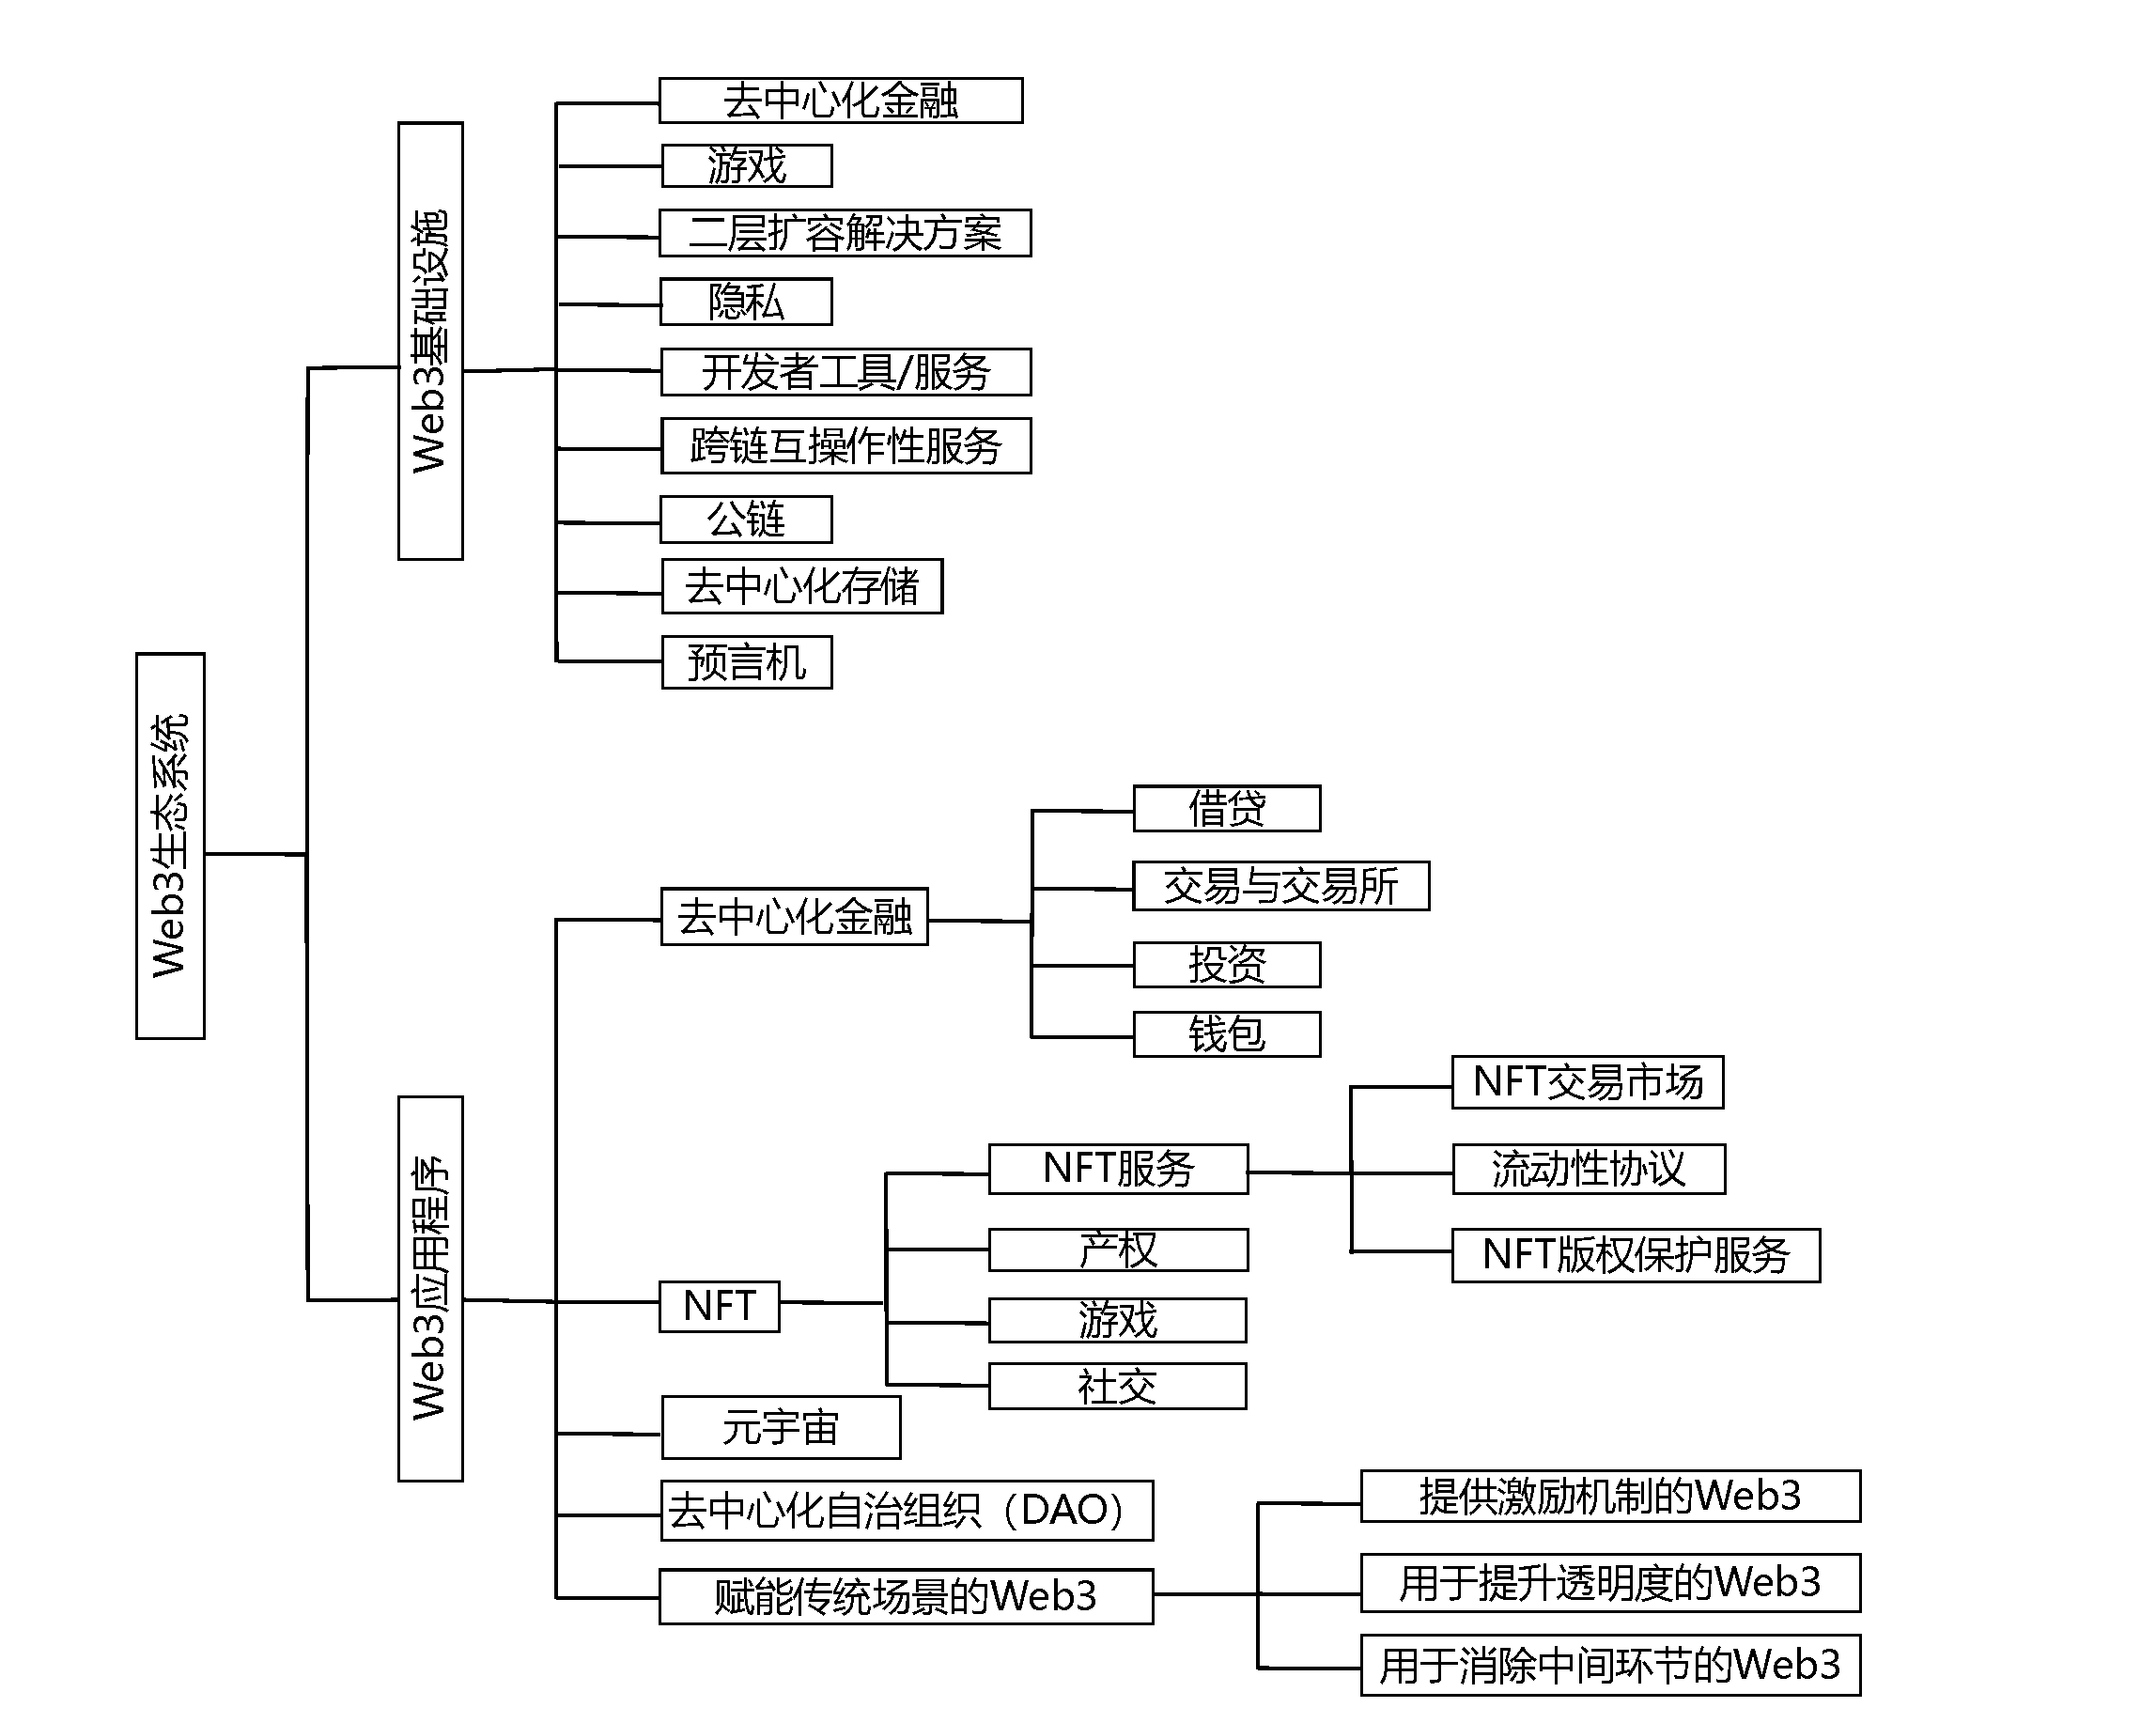
\includegraphics[width=1.1\linewidth]{./figures/web3_ecosystem.pdf} 
    \caption{Web3生态系统}
    \label{Fig:web3ecosystem}
\end{figure}


\subsection{Web3基础设施}
Web3基础设施涵盖了各种为开发者提供开发支持并增强区块链网络功能的解决方案。我们的分析确定了Web3基础设施的九个子类：去中心化金融~\cite{jensen2021introduction}基础设施、游戏基础设施、二层扩容解决方案~\cite{sguanci2021layer}、隐私基础设施、开发者工具/服务、跨链互操作性服务~\cite{pillai2020cross}、公链、去中心化存储~\cite{benisi2020blockchain}以及预言机~\cite{pasdar2023connect}服务。接下来，我们将详细介绍每一个子类，以及子类中有代表性的Web3项目。


\textbf{1.去中心化金融基础设施}

去中心化金融基础设施通过提供标准化的API或软件开发工具包来简化代币兑换功能的开发流程。

在去中心化金融基础设施领域，0x是一个具有代表性的项目~\cite{0x}。该项目在以太坊及多个兼容以太坊虚拟机的区块链上部署了支持ERC-20代币兑换的智能合约~\cite{erc-20}，这些合约能够聚合来自诸如Uniswap等去中心化交易所的流动性~\cite{uniswap, malamud2017decentralized}。此外，0x协议向开发者提供了用于实现代币兑换功能的标准化API，使其能够便捷地将该功能集成至Web3应用中，并共享来自多个交易平台的聚合流动性。


\textbf{2.游戏基础设施}

游戏基础设施能够协助缺乏区块链经验的开发者，将游戏内虚拟资产有效整合至区块链系统中。

Enjin~\cite{enjin}是该领域内具有代表性的项目之一，它支持开发者使用C/C++、Java和Python等主流编程语言进行游戏开发。通过Enjin，开发者可以创建虚拟资产，并为其分配相应的链上代币。Enjin提供的API接口使得这些代币能够顺利集成进游戏系统中。此外，Enjin还负责接收并监控来自游戏的相关请求，在区块链上完成处理后将结果返回游戏，实现链上链下的无缝对接


\textbf{3.二层扩容解决方案}

区块链网络吞吐量有限，成为制约Web3应用大规模部署的关键瓶颈。二层扩容方案在不修改底层协议的前提下提升网络处理能力，常见方法是在链下执行交易，仅将精简后的摘要信息上传至主链，从而缓解主链负载。

Optimistic Rollups是其中的典型代表，已被如Optimism~\cite{optimism}等以太坊虚拟机兼容网络广泛采用。该方案在二层打包并压缩多笔交易，默认其有效后统一提交至主链~\cite{schaffner2021scaling, chauhan2018blockchain}。任何节点在发现可疑交易时可提出欺诈证明发起挑战，验证失败将触发惩罚机制。该设计在提升系统吞吐量的同时维持了交易的正确性与网络的安全性。


\textbf{4.隐私基础设施}

在大多数区块链网络中，用户数据是公开可见的，这对用户隐私构成了挑战。隐私基础设施的核心在于防止交易记录暴露，降低用户身份与行为关联的风险。

Aztec Protocol~\cite{aztec}是典型的隐私基础设施之一，由一个以太坊智能合约和一个基于零知识证明技术的二层网络构成~\cite{sun2021survey}。用户将代币存入其智能合约后，资产被转移至Aztec的二层网络。在该网络中，用户可以私下转账或与接入Aztec的一层智能合约进行交互。所有交易以零知识简洁非交互式知识论证~\cite{petkus2019and}的形式表示，有效避免交易数据泄露。交易随后被打包并提交至以太坊主链。开发者可调用Aztec提供的API，将其智能合约与该协议集成，使Web3应用支持用户隐私交互。


\textbf{5.开发者工具/服务}

开发者工具和服务用于支持智能合约的开发、测试、部署与管理，提升开发效率并降低技术门槛。

ConsenSys~\cite{consensys}是该领域中广受采用的项目，旗下包括Infura~\cite{infura}和Truffle~\cite{truffle}等核心组件。Infura作为以太坊节点服务提供商，使开发者无需自建节点即可连接至以太坊网络，并提供账户管理、智能合约部署、交易签名与链上数据访问等API接口。Truffle则是一个完整的以太坊开发框架，涵盖合约编译、测试、部署以及交互式控制台功能，并配套提供用于Web3应用开发的相关库，构成高效的开发环境。


\textbf{6.跨链互操作}

区块链之间缺乏原生通信机制，导致数据与价值在多链环境中的流动受到限制。跨链互操作解决方案用于打通这一隔阂，支持不同区块链系统间的信息与资产交互。

Axelar~\cite{axelar}是该领域中应用广泛的代表，其作为一个独立的去中心化网络运行，拥有专属验证节点。该网络在连接的各条区块链上部署智能合约，形成互操作桥梁。合约由采用多方密码学的共享密钥控制，密钥被拆分并分配给各验证节点，持有份额与其质押的Axelar代币数量挂钩。验证节点在目标链上运行全节点，负责监测链上活动。当检测到用户向Axelar合约存入资产时，节点对跨链转移请求进行审批；一旦共享密钥中超过半数份额同意，合约即执行跨链转账操作。


\textbf{7.公链}

公链在设计上面临区块链不可能三角的结构性挑战~\cite{monte2020scaling}，即难以在去中心化、可扩展性与安全性三者之间同时取得平衡。

为在保证安全性的前提下提升可扩展性，多个公链正探索技术路径。NEAR~\cite{near}是一个具有代表性的项目，它提出通过名为Nightshade~\cite{skidanov2019nightshade}的分片技术~\cite{wang2019sok}来提高可扩展性。在该技术中，每个区块根据分片数量被拆分为多个数据块，由不同分片分别处理。网络通过可验证随机函数~\cite{micali1999verifiable}将各分片分配给部分验证节点。每个节点仅需存储并验证对应分片的数据块，而非完整区块，从而显著降低资源消耗，增强系统可扩展性。


\textbf{8.去中心化存储}

在以太坊等主流区块链网络中，数据需在所有节点上同步存储，导致存储成本显著上升。为缓解这一问题，去中心化存储网络应运而生，其运行机制在结构上与区块链相似。用户文件经过加密后分布式存储于网络节点，仅加密元数据（如文件位置和哈希值）被写入链上，从而避免将完整文件纳入区块，降低了成本。

Filecoin~\cite{filecoin}是建立在星际文件系统（IPFS）协议~\cite{benet2014ipfs}基础上的代表性项目。在该网络中，用户依据文件大小和存储时长支付费用，文件随后被分配至多个存储节点。为证明文件在约定时间内持续存在且未被篡改，节点需提交由文件生成的时空证明~\cite{moran2016proofs}与复制证明~\cite{benet2017proof}，以确保存储过程的可验证性和完整性。


\textbf{9.预言机}

预言机（Oracle）作为链下与链上之间的接口，用于将外部数据引入区块链，供智能合约调用。然而，若引入的数据无效或具恶意，可能对合约执行及用户资产构成威胁。

Razor Network~\cite{razor}提出一套激励与惩罚机制以提升数据可信度。数据提供者需质押代币作为担保，提交有效数据可获得奖励，提交无效数据则面临惩罚。这一机制强化了数据提供的诚实性，有助于保障智能合约运行的正确性及用户资产的安全性。


\subsection{Web3应用程序}
Web3应用程序是一类面向用户构建的去中心化应用集合。在本研究中，Web3应用被划分为五个子类别：去中心化金融（DeFi）、非同质化代币（NFT）、元宇宙、去中心化自治组织（DAO），以及面向传统场景的Web3应用。其中，DeFi、NFT与传统场景应用内部还包含多个细分类型，以下将分别展开论述。


\textbf{1.去中心化金融}

去中心化金融指的是运行在区块链之上的去中心化金融系统。在我们的数据集中，去中心化金融子类进一步细分为四个更小的子类：\textbf{i.借贷；ii.交易与交易所；iii.投资；以及 iv.钱包}。接下来，我们将对每个子类进行详细介绍。

\textbf{i.借贷。}借贷协议通过聚合多个贷方的资金，为借款方提供贷款服务，并从中收取利息作为贷方的收益来源。

Aave~\cite{aave}是该领域中的代表性协议，支持超额抵押借贷与闪电贷两类服务。在超额抵押借贷中，借款者需预先锁定价值高于贷款金额的加密资产作为抵押。若抵押资产价值跌破设定阈值，智能合约将自动发起清算流程，以回收资金并保障贷方利益。闪电贷~\cite{wang2020towards}面向具备编程能力的开发者，提供无需抵押的短时借贷。借款者需在单笔交易完成前偿还全部借款及利息，未按时偿还将导致交易整体回滚，确保资金安全。

\textbf{ii.交易与交易所。}
交易与交易所类应用程序主要包括一系列去中心化交易所，支持用户在链上进行代币兑换，无需依赖中心化托管方。而传统中心化交易所普遍采用订单簿机制~\cite{abudy2018corporate}，但在链上环境中，该模式通常效率较低，难以适应高频交易需求。

Uniswap是该领域的代表性项目，其采用自动做市商（AMM）算法~\cite{xu2021sok}替代传统订单簿机制。该算法基于流动性池运行，允许用户在无需等待撮合的情况下即时完成代币互换。兑换比例由池中两种代币的存量比例决定，遵循预设的定价函数，有效提升了交易效率与系统的去中心化程度。币兑换，使用户能够实现即时的代币互换。兑换比例是通过一种特定算法，根据池中两种代币的比例来确定的。

\textbf{iii.投资。}
投资协议在去中心化环境中承担类似投资基金的角色，将交易策略以代码形式嵌入智能合约中。用户将资金存入智能合约后，系统按照预设规则执行交易操作，产生的收益再按比例分配给用户。

TokenSets~\cite{tokensets}是该领域中应用广泛的协议，为用户提供多样化的投资组合。每个组合由一个智能合约管理，根据既定策略在去中心化交易所中对特定代币进行交易。该平台还支持用户自行定义投资策略并部署为智能合约，向其他用户公开，以实现策略共享与资产增值的双重目标。

\textbf{iv.钱包。}
钱包是用于管理加密资产并与Web3应用交互的工具，为用户提供账户控制与交易签名等功能。

MetaMask~\cite{metamask}是最为广泛使用的钱包之一，支持用户在多种设备上通过助记词创建或恢复以太坊账户，避免直接管理复杂的公私钥对。用户可使用MetaMask管理ERC-20代币，并与各类Web3应用无缝连接，完成资产转账、智能合约调用等操作。



\textbf{2.NFT}

NFT子类代表一类融合了非同质化代币元素的Web3应用~\cite{wang_non-fungible_2021}，可进一步划分为四个细分方向：\textbf{i. NFT服务；ii. 产权；iii. 游戏；iv. 社交}。以下将分别对各子类别进行详细介绍。

\textbf{i.NFT服务。}该方向包含以下三个更小的子类：\textbf{a.NFT交易市场；b.流动性协议；c.NFT版权保护服务}。


\textbf{a.NFT交易市场。}
NFT交易市场是专门用于非同质化代币买卖的平台。

OpenSea~\cite{OpenSea}是当前规模最大的NFT交易市场，支持用户交易多种类型的NFT资产，包括艺术品、音乐和游戏道具等。平台还提供铸造功能，允许用户在不具备区块链技术背景的情况下生成并发布自己的NFT。
	
    
\textbf{b.流动性协议。}
NFT通常价格较高，且存在流动性不足的问题。

为应对这一挑战，fractional.art~\cite{fractional}提出了基于所有权分割的流动性提升方案。该方法将NFT锁定在平台提供的智能合约中，并基于该资产发行多个ERC-20代币，每个代币对应NFT的一定比例所有权。此机制在保持资产完整性的同时，降低了投资门槛，有助于提升NFT的市场流动性。
	
    
\textbf{c.NFT版权保护。}
NFT市场频繁遭遇假冒问题，恶意用户常通过上传知名NFT的图像并重新铸造新NFT进行挂牌销售，扰乱市场秩序并侵犯原始作品版权。

Doppel~\cite{doppel}项目针对这一问题提出检测机制，利用计算机视觉与人工智能模型识别假冒NFT，并支持用户进行举报。目前，该系统已覆盖以太坊、Solana和波场等多个区块链平台，为NFT版权保护提供技术支持。


\textbf{ii.产权。}
NFT已被用于数字和实体产权的标识与保护。

在数字产权领域，Royal.io~\cite{Royal}提供基于NFT的音乐版权管理服务。艺术家可在平台上为其作品铸造NFT，并将歌曲名称、哈希值及版税分配比例嵌入至元数据中。当歌曲被他方使用或购买时，NFT持有者可按设定比例获得相应版税收益。在实体资产方面，Origyn~\cite{origyn}将实物资产（如手袋、手表与珠宝）的高清图像铸造成NFT，用作所有权凭证，从而在链上确权实体资产。


\textbf{iii.游戏。}
NFT技术已在游戏行业中得到应用，游戏内虚拟资产被铸造成NFT，使玩家重新获得对游戏数据的所有权。这类融合资产机制的游戏通常被称为“游戏化金融”，玩家在参与过程中有机会获得经济收益。

Axie Infinity~\cite{noauthor_axie_nodate}是该领域具有代表性的项目，玩家可在其中收集、繁育、饲养并交易虚拟宠物。每个宠物以NFT形式存在于区块链上，具备独立的所有权和市场价值。玩家既可以操控宠物参与对战，也可以将其出售以获取通证奖励，实现游戏与收益的结合。


\textbf{iv.社交。}
NFT技术已延伸至社交领域，为用户提供在不依赖中心化平台控制的前提下进行自我表达的手段。

Mirror~\cite{mirror}是该子类中的代表性项目，作为去中心化博客平台，允许用户发布内容并将其铸造成NFT。内容被存储在星际文件系统上，从而避免因平台干预导致的数据篡改或删除。用户还可购买创作者发行的NFT，以表达支持并参与内容生态的构建。

\textbf{3.元宇宙}

元宇宙~\cite{gadekallu2022blockchain}指由计算机系统构建的虚拟空间，可与现实世界交互融合，形成持续存在的数字环境。

许多元宇宙项目以区块链为基础，特点是在虚拟世界中将角色或资产铸造成非同质化代币（NFT）。The Sandbox~\cite{thesanbox}是面向虚拟地产的代表性项目，用户可在平台地图上购买土地并进行自主开发。这些土地以NFT形式记录在区块链上，具备明确的所有权，同时用户还可自由访问和浏览他人所构建的虚拟空间。 


\textbf{4.去中心化自治组织}

DAO（去中心化自治组织）~\cite{axelsen2023dao}是一种基于智能合约运行的组织形式，依靠预设规则自动执行治理与管理操作。

CreatorDAO~\cite{creatordao}是该领域的代表性项目，将投资者、创作者与支持者聚合于同一社区。该组织为创作者及其项目提供资金和资源支持，推动创作活动的发展。当作品产生收益时，智能合约依据既定规则自动完成利润分配，确保社区成员按其贡献获得相应回报。


\textbf{5.赋能传统场景的Web3}

Web3技术也已被许多传统行业所采用，以应对与激励机制、协作、透明度、信任等相关的挑战。基于Web3在传统行业中的功能，我们确定了三个子类别：\textbf{i.提供激励机制的Web3；ii.用于提升透明度的Web3；iii.用于消除中间环节的Web3}。


\textbf{i.提供激励机制的Web3。}
一些传统行业已开始在去中心化网络基础上开展业务，借此引入Web3提供的激励机制。

例如，Helium~\cite{helium}是一个基于区块链的无线网络运营平台。其向用户出售设备，用于提供网络覆盖和参与挖矿。用户部署设备后可获取通证奖励，作为其贡献网络资源的回报。该模式在降低企业基础设施建设和运营成本的同时，也使用户能够在传统通信场景中获得实际收益。


\textbf{ii.用于提升透明度的Web3。}
部分传统行业已引入Web3技术，将关键业务信息记录在区块链上，以增强透明度并解决信任问题。

Green Labs~\cite{greenlabs}和Blocery~\cite{blocery}为应用区块链于产品追溯的案例。它们将生产时间、流转路径和销售记录等核心数据上链，利用区块链公开、不可篡改的特性，实现从生产到销售全过程的可验证追溯。这一机制增强了信息透明度，有助于建立用户与企业之间的信任关系。


\textbf{iii.用于消除中间环节的Web3。}
Web3借助智能合约自动执行业务流程，省去了传统商业模式中对中介机构的依赖。

例如，Dtravel~\cite{dtravel}是部署在以太坊上的去中心化旅游平台，旅行者可直接与房产所有者通过智能合约完成预订，无需借助在线旅行社。该模式减少了中间环节，提高了交易效率与用户自主性。


\section{Web3代码和市场数据收集与分析}
本小节介绍了收集Web3项目中与代码和与市场相关数据的方法，以及相应的数据分析方法，以揭示Web3项目的流行度。

\subsection{代码和市场数据收集}
我们首先通过GitHub收集了Web3项目在Github的代码相关数据，然后通过Web3区块链浏览器（如Etherscan~\cite{etherscan}、Bscscan~\cite{bscscan}和Polygonscan~\cite{polygonscan}）收集了Web3项目的市场相关数据。

对于代码相关数据，我们首先人工检查Web3项目是否在GitHub上有开源代码库。在人工审查了200个Web3项目后，我们确定了96个开源的Web3项目。然后，我们通过爬虫收集了所确定的这96个项目在GitHub中的代码相关数据（代码行数和提交次数）。

对于市场相关数据，我们利用区块链浏览器的API获取了每个Web3项目在2022年1月至2023年1月期间的交易数和市值数据（包括市值和唯一钱包数）。


\subsection{代码层面的流行度分析}
对于Web3基础设施和Web3应用程序的每个子类，我们计算了开源项目的数量，以及所有项目的代码存储库的代码总行数和提交次数（见表~\ref{Table:githubdata}），这些数据用于从代码层面量化特定子类的流行度。项目数量更多、代码行数更多且提交次数更多的子类别被认为更受欢迎。

此外，我们分析了每个Web3项目所使用的编程语言以及部署的区块链平台。然后，我们总结了每种编程语言的使用频率以及部署在不同区块链平台上的Web3应用程序数量，以了解编程语言和区块链平台的流行度。


\begin{table}[!htbp]
\centering
\caption{Web3项目的代码相关数据}
\label{Table:githubdata}
\vspace*{-0.25cm}
\tabcolsep=16.5pt
\begin{tabular}{lcll}
\hline
\textbf{子类别} & \textbf{项目数量} & \textbf{代码行数} & \textbf{提交次数} \\
\hline
公链 & 17 & 3,386,348 & 124,040 \\

跨链互操作性 & 9 & 3,156,655 & 39,720  \\

开发者工具 & 8 & 641,749 & 11,998  \\

去中心化存储 & 7 & 421,291 & 17,708  \\

预言机 & 3 & 364,499 & 872  \\

游戏基础设施 & 2 & 309,826 & 6,330  \\

Layer 2 扩展方案 & 2 & 2,071,208 & 15,594  \\

隐私保护 & 2 & 436,352 & 7,960  \\

DeFi 基础设施 & 1 & 105,496 & 17,137  \\

借贷 & 12 & 595,999 & 11,205  \\

交易与兑换 & 7 & 214,912 & 2,756   \\

投资 & 4 & 80,193 & 2,919  \\

DAO & 1 & 2,793 & 55   \\

钱包 & 2 & 162,163 & 4,533  \\

NFT 市场 & 2 & 117,305 & 2,977  \\

NFT 流动性 & 2 & 56,843 & 454  \\

NFT版权保护 & 1 & 14,091 & 3 \\

产权类 & 2 & 105,070 & 806  \\

游戏 & 3 & 28,002 & 162   \\

元宇宙 & 1 & 462,462 & 5,656  \\

提供激励机制的Web3 & 2 & 98,049 & 3,804 \\

消除中间环节的Web3 & 4 & 20,992 & 321  \\
\hline
\end{tabular}
\vspace*{-0.5cm}
\end{table}





\begin{table}[!htb]
\centering
\caption{Web3项目的市场相关数据}\vspace*{-0.25cm}
\tabcolsep=14.5pt
\begin{tabular}{llll}
\hline
\textbf{子类别} & \textbf{项目数量} & \textbf{用户数} & \textbf{市值} \\
\hline
借贷 & 14 & 129,188 & \$1,827,265,578   \\

交易与兑换 & 11 & 843,178 & \$5,831,446,783  \\

投资 & 2 & 22,287 & \$2,682,758,809 \\

NFT 市场 & 4 & 2,070,447 & \$24,687,589,059  \\

产权类 & 4 & 16,422 & \$28,864,897  \\

游戏 & 17 & 193,249 & \$1,249,040,083  \\

社交 & 3 & 18,780 & \$8,753,611  \\

元宇宙 & 1 & 220,532 & \$950,498,005  \\

DAO & 4 & 49,375 & \$1,177,325,522   \\

提供激励机制的Web3 & 3 & 477,043 & \$522,377,779  \\

消除中间环节的Web3 & 2 & 2,910 & \$16,049,029 \\

\hline
\label{Table:marketdata}
\end{tabular}
\end{table}



\subsection{市场层面的流行度分析}
我们将Web3项目划分为两组：一组部署在多个区块链平台上，另一组仅部署在单一平台上。每组均包含项目名称、用户数量及市值数据。通过比较两组的用户数量中位数和市值中位数，并参考其最大值，评估部署在多个平台与单个平台之间在用户覆盖和市值表现上的差异。

采用相同方法，将Web3项目进一步划分为开源与非开源两类，并分别计算其用户数量和市值的中位数与最大值，以分析开源策略对项目影响的具体体现。

此外，针对Web3项目的各个子类，统计了每类应用的用户总数与总市值（见表~\ref{Table:marketdata}），以从市场维度衡量其受欢迎程度。最后，对各Web3应用的用户数量进行了分布分析，图~\ref{Fig:uaws}展示了相关统计结果。


\section{Web3项目的流行度}
本小节从代码层面与市场层面分析了Web3项目的流行度，相关结果有助于从业者与研究人员识别Web3生态中的开发者偏好与技术趋势，以及了解用户对不同类型应用的接受程度及其不同类型应用的市场价值。


\subsection{代码层面的流行度}
代码层面的研究结果揭示了开发者偏好与项目流行度之间的关系，反映出不同类型Web3基础设施与应用在开发实践中的受关注程度，以及开发者在部署平台选择上的倾向。

表~\ref{Table:githubdata}汇总了Web3项目的代码相关数据，首列列示了开源项目的子类别，其中第1至第9行对应Web3基础设施，第10至第21行对应Web3应用。图~\ref{Fig:platformdistribution}进一步展示了这些项目在各区块链平台上的分布情况。基于表中数据，可归纳出以下观察发现：

 \begin{figure}[!htbp]
 \centering
		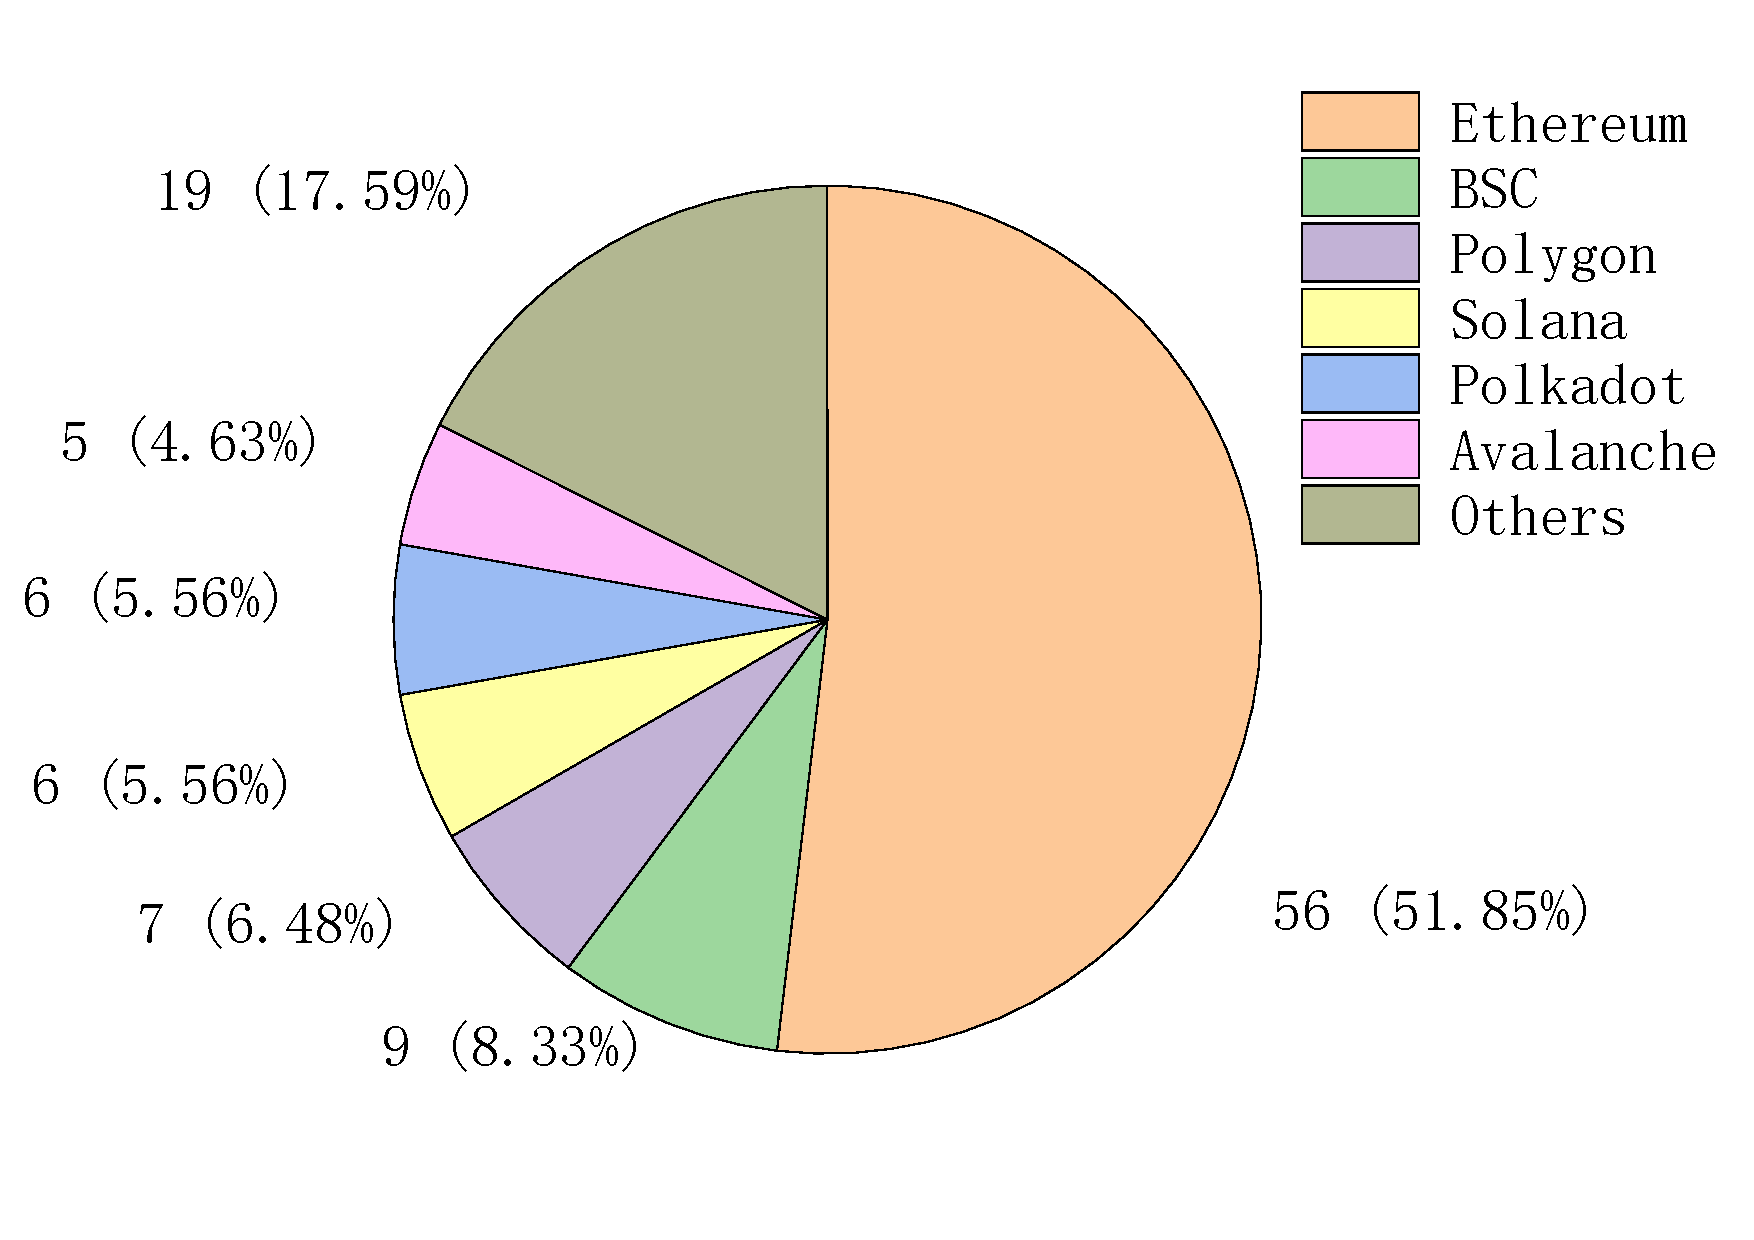
\includegraphics[width=0.6\textwidth]{./figures/platform2.pdf} 
        \vspace*{0.25cm}
		\caption {Web3项目在不同区块链网络的分布} 
		\label{Fig:platformdistribution}
\end{figure} 


\textbf{1. 公链在Web3基础设施中具有最高的开发活跃度。}

如表~\ref{Table:githubdata}所示，开源Web3基础设施项目中，公链类项目数量最多，共17个。此外，该类别在代码行数（3,386,348行）和提交次数（124,040次）方面排名最高，反映出其在开发者中的开发活积极性最高。

\textbf{2. 借贷类应用在Web3应用开发中表现出最高活跃度。}

根据表~\ref{Table:githubdata}，在Web3应用的各子类别中，借贷类项目的开源数量为12个，为数量最多的一类。同时，该类别的代码行数为595,999行，提交次数为11,205次，均高于其他子类别，显示出该领域在开发中的活跃程度最高。


\textbf{3.以太坊是部署Web3应用最主要的网络。}

如图~\ref{Fig:platformdistribution}所示，在108个Web3应用中，56个部署在以太坊网络，占比51.85\%。相比之下，其他区块链网络上的Web3应用数量在5至19之间，占比介于4.63\%至17.59\%。该数据表明，以太坊在智能合约部署方面具有较强的吸引力。



\textbf{4.Solidity~\cite{dannen2017solidity}是智能合约开发中最广泛使用的编程语言。}\label{solidity_37}

在41个开源Web3应用中，有37个采用Solidity作为智能合约开发语言，表明该语言在Web3应用开发中受到开发者的广泛青睐。



\subsection{市场层面的流行度}
市场层面的研究结果揭示了Web3应用在用户活跃度和市场认可度方面的表现。这些发现有助于识别用户规模较大、市值水平较高的应用特征，并分析在Web3生态中较受欢迎的活动类型及其用户增长趋势。

图~\ref{Fig:2-1}展示了Web3应用的用户数量与市值分布情况，图~\ref{Fig:uaws}呈现了2022年1月至2023年1月期间的用户增长曲线。表~\ref{Table:marketdata}则汇总了各项目的市场数据。基于上述信息，可得出以下观察发现：

\textbf{1.多链部署的Web3应用拥有更多用户和更高市值。}

如图~\ref{Fig:2-1}(a)所示，第一个和第二个箱形图分别展示了多链部署与单链部署Web3应用的市值分布。多链部署应用的市值中位数和最大值均高于单链部署，反映出其在市场价值层面的相对优势。

类似趋势也体现在用户数量上。图~\ref{Fig:2-1}(b)中的箱形图对比了两类部署方式下的用户数量分布，多链部署的应用在中位数和最大值上均优于单链部署，表明其用户覆盖范围更广，活跃度更高。

\begin{figure}[!htbp]
\centering
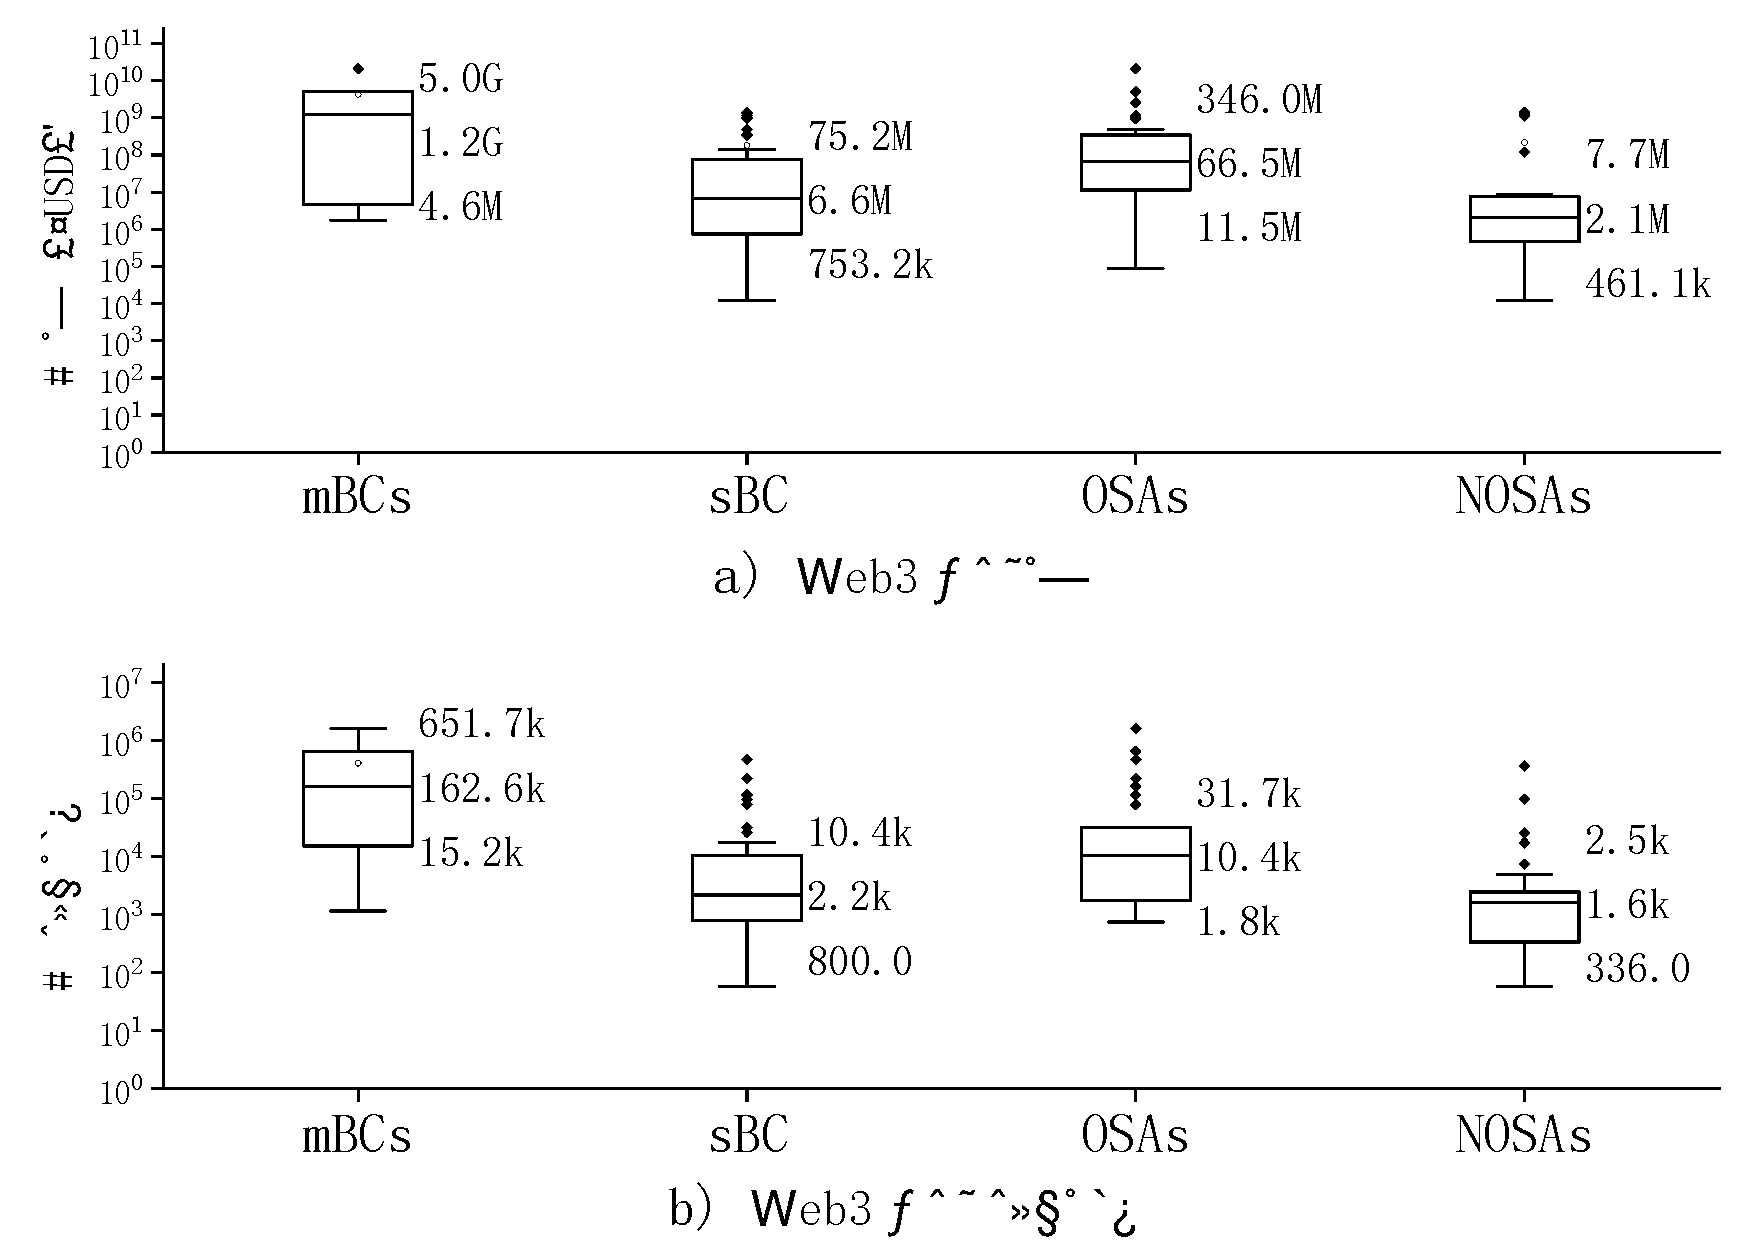
\includegraphics[width=0.8\textwidth]{./figures/2-1.pdf} 
\caption[用户数量与市值的分布情况]{用户数量与市值的分布情况。\textbf{mBCs}表示多链部署的应用程序。\textbf{sBC}表示单链部署的应用程序。\textbf{OSAs}表示开源应用程序，而\textbf{NOSAs}表示非开源应用程序。}
\label{Fig:2-1}
\end{figure}




\begin{figure}[!htbp]
\centering
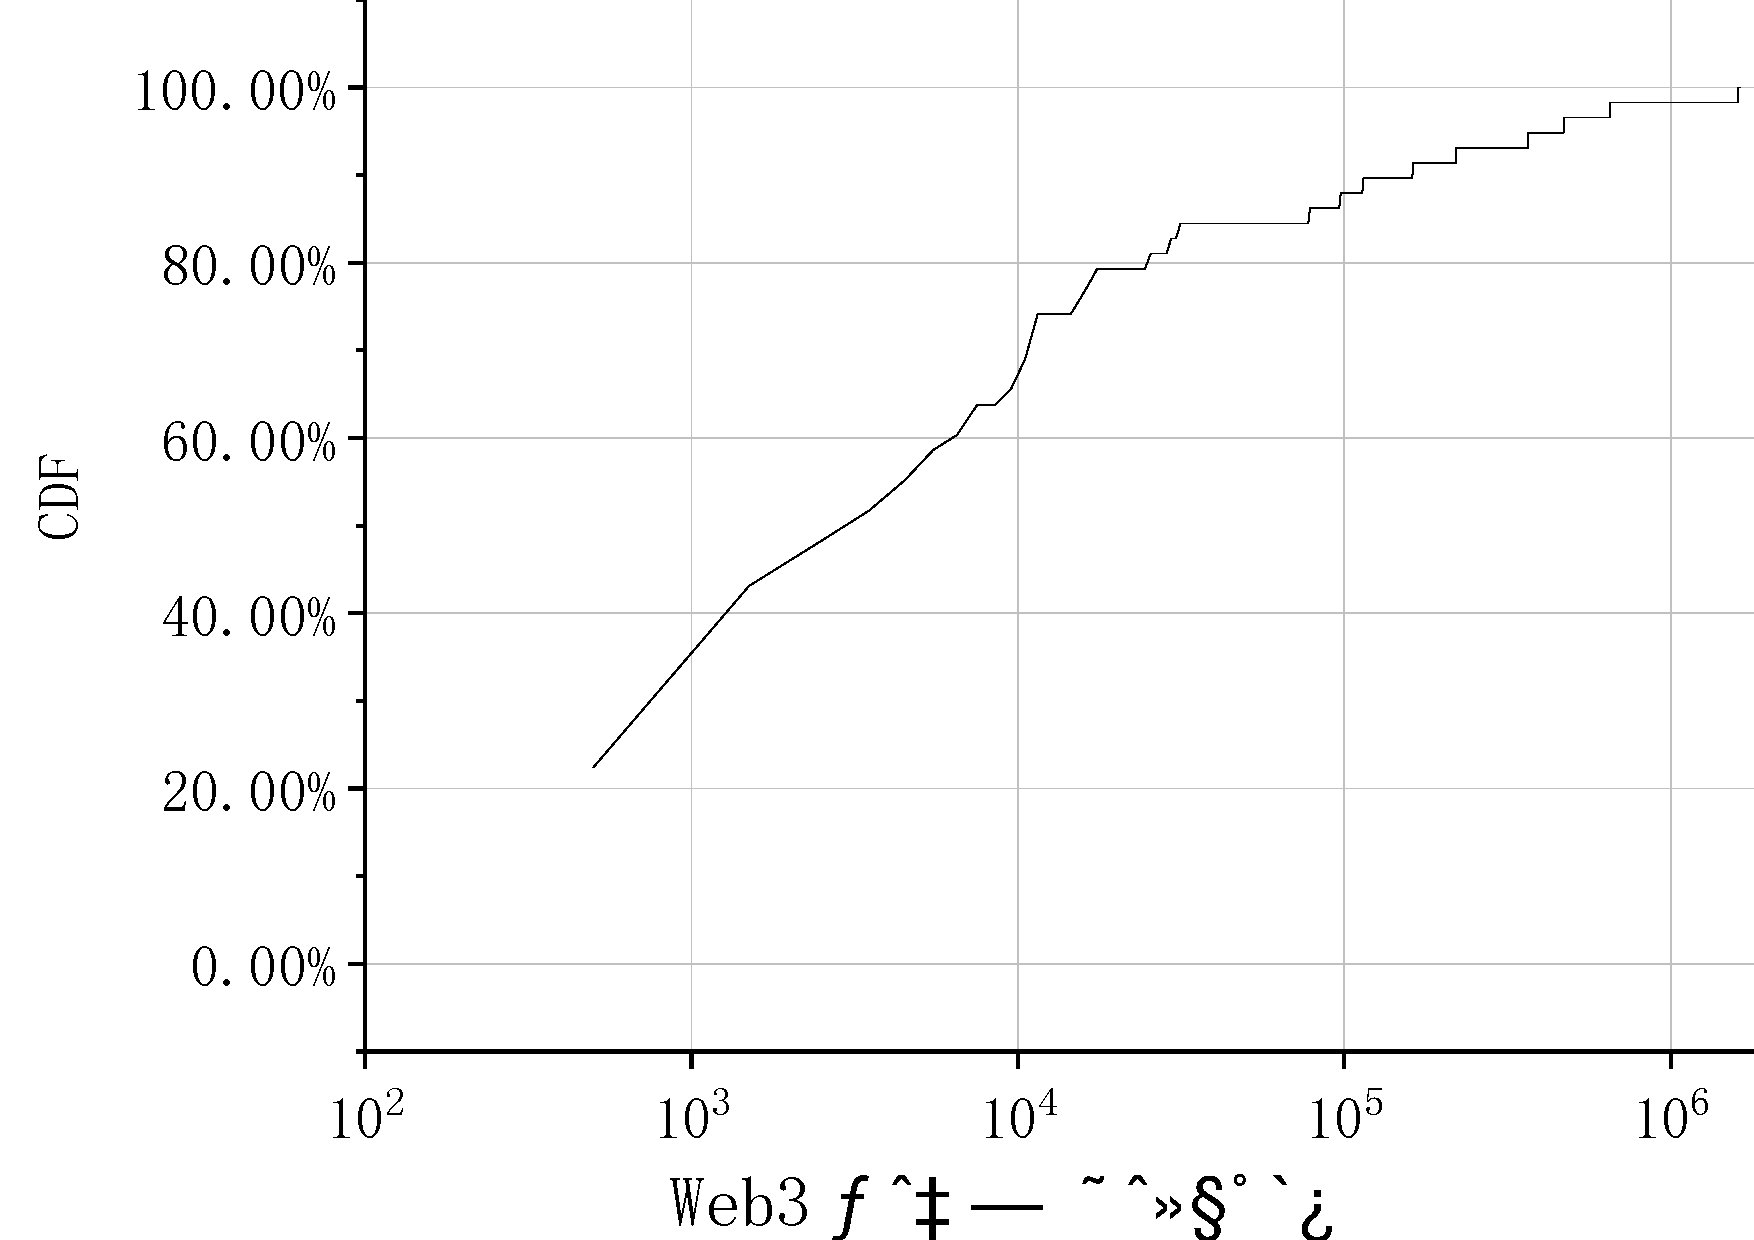
\includegraphics[width=0.6\textwidth]{./figures/uaws.pdf} 
\caption[Web3应用程序的用户数量]{2022年1月到2023年1月期间Web3应用程序的用户数量。}
\label{Fig:uaws}
\end{figure}







\textbf{2.开源Web3应用在用户吸引力和市值方面表现更为突出。}

图~\ref{Fig:2-1}(a)中的第三与第四个箱形图分别展示了开源与非开源Web3应用的市值分布。结果显示，开源应用的市值中位数和最大值均高于非开源项目。这一差异可能反映出开源带来的透明度、社区参与度以及用户信任水平在提升市场认可度方面的积极作用。

图~\ref{Fig:2-1}(b)进一步呈现了两类项目的用户数量分布。开源应用的用户数量最大值显著高于非开源应用，后者的用户数量中位数相对较低，表明开源项目在用户层面具备更强的吸引力和增长潜力。


\textbf{3.NFT交易是Web3生态系统中用户最活跃的子类。}

如表~\ref{Table:marketdata}所示，NFT市场的用户数量为2,070,447，位居各应用类别之首，其市值也达到24,687,589,059美元，处于较高水平。这一结果表明，NFT交易是Web3中最受用户欢迎的应用。



\textbf{4.约65\%的流行Web3应用在2022年至2023年期间用户增长数未超过10,000。}
图~\ref{Fig:uaws}展示了2022年1月至2023年1月期间，热门Web3应用累计独立用户数量的累积分布函数。数据显示，大约65\%的应用在一年内的新增用户数量未超过10,000。这一趋势揭示了Web3在用户获取上的挑战，同时也体现了该领域整体仍处于发展初期。


\section{Web3智能合约的问题报告收集与分析}
Web3问题报告是指开源Web3项目在Github的问题报告。本小节主要介绍通过Github收集Web3项目的问题报告方法，以及如何使用大语言模型分析这些问题报告，以便洞察和识别Web3中可能存在的漏洞及开发者对待漏洞的处理方式。


\subsection{Web3智能合约问题报告收集}
在本小节，我们首先筛选了175个包含问题报告的开源Web3项目仓库，然后开发了一款爬虫程序，从这些仓库中爬取了1175条问题报告。具体步骤如下。

\textbf{步骤一：识别包含问题报告的Web3项目仓库}

首先，我们从获得风险投资的200个Web3项目中筛选出23个在GitHub平台上包含问题报告的项目。然而，由于该数量较为有限，难以全面反映Web3领域的问题，因此，为了进一步扩大数据规模、提升问题报告的覆盖率，并确保所收集数据的广泛性和代表性，我们利用GitHub的高级搜索功能，以“Web3”为关键词进行检索，额外识别出152个包含问题报告的开源Web3项目仓库。

具体而言，我们开发了一款爬虫脚本，用于自动识别GitHub上包含问题报告的项目仓库。数据筛选过程包括以下几个步骤：

\textbf{1.关键词与筛选条件}：采用“Web3”作为核心关键词，并将Solidity设定为编程语言的筛选条件。Solidity的选取基于其在Web3智能合约开发中的广泛应用。在章节~\ref{solidity_37}的发现中显示：41个开源Web3应用中，有37个使用Solidity语言编写其后端智能合约。

\textbf{2.数据排序与筛选}：在搜索结果中，我们按照Star数量降序排列，并获取前100页的搜索结果（GitHub的搜索功能仅允许访问前100页的结果）。

\textbf{3.问题报告筛选}：在获取的GitHub仓库列表中，我们在项目链接后附加"/issues?q=is\%3Aissue"以筛选出包含问题报告的仓库。

经过上述筛选流程，我们最终确定了175个包含问题报告的Web3项目仓库。



\textbf{步骤二：收集问题报告}

在确定了包含问题报告的175个Web3项目仓库后，我们开发了一款自动化爬虫脚本，从这些仓库中收集到了1175个问题报告。
具体而言，对于每条问题报告，我们提取以下关键信息：

\textbf{标题}：问题报告的概述，通常由开发者对问题的简要描述。

\textbf{正文}：详细的错误信息，例如漏洞的描述或者漏洞代码。

\textbf{评论}：开发者针对问题的讨论、分析以及修复方案。

所有数据均以结构化JSON格式存储，每条记录包含title、body和comments三个核心字段，以便后续自动化分析与人工审查。

需要注意的是，在数据采集过程中，我们仅爬取了已关闭的问题报告，并过滤掉开放中的问题报告。此选择主要基于以下考虑：

1. 开放的问题报告仍处于讨论阶段，其中提及的漏洞尚未得到充分验证，可能包含大量不确定性信息。

2. 已关闭的问题报告通常包含更高质量的讨论，并附有开发者的反馈与完整的修复过程，从而有助于准确理解Web3项目中的常见问题及其解决方案。

最终，我们成功从175个Web3项目仓库中爬取了1175个问题报告。



\subsection{基于大语言模型分析问题报告}
在问题报告收集完成后，我们调用了大语言模型DeepSeek\_v3的API，并设计了一条结构化提示词对问题报告进行自动化分析。目的是高效识别漏洞相关问题、总结问题核心内容、对潜在漏洞进行分类以及归纳开发者对漏洞的讨论，具体提示词如图~\ref{fig:prompt-issue-analysis}所示。


\begin{figure}[H] 
\centering
\begin{tcolorbox}[
  enhanced,
  breakable=false,   
  colback=gray!10,
  colframe=black,
  boxrule=0.5pt,
  arc=0pt,
  left=5pt,
  right=5pt,
  top=5pt,
  bottom=5pt,
  title={问题报告分析提示词模板},
  fonttitle=\bfseries
]

\#\#\# Github 问题报告信息：

标题: \{title\}  

正文: \{body\}  

\#\#\# 请基于问题报告的标题和正文回答以下问题：  

1. 该问题是否涉及漏洞？  
2. 若涉及漏洞，总结该问题的核心内容。  
3. 若涉及漏洞，请分类漏洞类型（如整数溢出）。  

开发者回复: \{comments\}  

\#\#\# 请基于 comments 总结开发者的讨论内容，并用以下JSON格式返回结果：

\{
  "original issue": \{
    
    "title": "原始问题标题",
    
    "body": "原始问题描述",
    
    "comments": ["comment 1", "comment 2", "comment 3"]
    
  \},
  
  "analysis": \{
  
    "is vulnerability": true,
    
    "summary": "...",
    
    "vulnerability type": "...",
    
    "cause analysis": "...",
    
    "developer comments": "..."
          \}
\}
\end{tcolorbox}
\caption{问题报告分析提示词模板}
\label{fig:prompt-issue-analysis}
\end{figure}




根据该提示词，大模型将依次执行以下自动化分析流程。首先，大模型基于问题报告的标题与正文提取并概括核心讨论内容。在此基础上，模型判断问题是否涉及漏洞；若涉及漏洞，则进一步对漏洞进行分类（如整数溢出、DOS攻击等）。随后，模型基于开发者的评论归纳其讨论内容，包括修复方案与争议焦点。最终，模型以结构化的JSON格式输出分析结果，具体包含原始问题数据及分析结论。分析结论涵盖对问题报告的核心总结、是否涉及漏洞的判断、漏洞类型、漏洞产生的可能原因以及开发者对待漏洞的观点。

基于上述自动化分析流程，我们对1175条问题报告进行处理，成功识别出280条涉及漏洞的问题报告。下一节中将对这些问题报告及模型返回的分析结果进行人工审查，进一步探讨漏洞类型及开发者对待漏洞的处理方式与观点。



\section{Web3智能合约漏洞}
在本小节中，我们对280条漏洞报告进行了人工分析，详细审查了每条报告的结构化信息，包括漏洞概要、漏洞类型以及漏洞成因。通过系统性归纳分析，我们发现Web3领域的漏洞主要可分为以下两类：

\textbf{(1) 通用漏洞}

此类漏洞通常源于区块链底层机制或智能合约代码实现中的共性问题，适用范围广泛，并非特定于某个具体应用或合约。攻击者可将同一漏洞利用方式复用于多个项目或协议中，因此造成的安全风险较大，具有明显的通用性，例如典型的整数溢出漏洞。

\textbf{(2) 业务逻辑漏洞}

此类漏洞通常源于特定合约或协议在业务逻辑设计上的缺陷，仅在特定的运行流程或交互模式下才会被触发，难以在其他协议中复用，因此缺乏普遍适用性。
例如，在借贷平台Aave的一个关于业务逻辑漏洞的问题报告指出，该平台的还款流程中支持用户使用持有的存款凭证（即代表存入资产的代币）直接偿还债务。但在这一流程中，系统未对用户的健康因子进行校验，攻击者可借此在资金不足、健康因子过低的情况下清除自身债务，同时制造系统内的坏账，从而非法提取资金。由于该漏洞依赖于Aave协议特有的还款机制与债务模型，难以在其他协议中复现，因此不属于通用漏洞。


基于上述分类，我们将研究聚焦于可能影响多个Web3应用程序或智能合约、具有较广泛攻击面的通用漏洞上。经过系统分析，我们总结出以下八类常见的通用漏洞。


\textbf{1.访问控制漏洞}

合约在权限管理方面存在设计或实现缺陷，导致未授权用户能够调用受保护的合约函数。此类漏洞通常源于访问修饰符配置不当或逻辑判断缺失，可能导致关键操作被绕过，引发资产被非法操作或敏感状态被篡改的风险。

\textbf{2.不安全随机数漏洞}

合约依赖可预测的链上数据（如区块哈希、时间戳等）生成随机数。由于这些数据可被区块生产者或攻击者部分控制，随机性不足将影响系统的公平性与安全性，尤其在涉及博弈、抽奖等场景中易被利用。

\textbf{3.整数溢出漏洞}

当运算结果超出数据类型的表示范围而未被检测时，会导致整数溢出或下溢。这类漏洞常见于代币合约中，可能引起余额异常、计算错误等问题，进而造成资产损失或状态异常。


\textbf{4.重入攻击漏洞}

攻击者在外部调用过程中通过递归调用目标合约函数，在其状态更新完成前多次触发关键逻辑，从而操纵或窃取合约资产。此漏洞通常与以太币转账函数配合使用的外部调用有关，是经典且高危的攻击路径。

\textbf{5.区块信息依赖漏洞}

合约依赖区块信息（如时间戳）作为关键逻辑的输入时，可能被矿工或验证者利用对区块生产过程的控制进行操控，从而改变合约行为。该问题破坏了合约逻辑的确定性与安全性。

\textbf{6.拒绝服务攻击漏洞}

攻击者利用构造极高gas消耗的输入、死循环或递归调用等方式，占用系统资源并阻碍合约正常执行。此类攻击会影响合约的可用性，甚至导致资金锁死或关键功能无法响应。


\textbf{7.未检查的外部调用漏洞}

合约调用外部合约函数后未验证其返回结果，若目标合约执行失败却未被调用方感知，可能导致关键逻辑被跳过或状态不一致，进一步引发安全漏洞。


\textbf{8.短地址攻击漏洞}

当合约未对输入地址参数进行有效性检查，尤其未正确处理长度不足或为全零地址（0x0）的情况，可能导致资产被错误转移、锁定或销毁。此漏洞通常与参数解析不严谨或对地址合法性假设不当有关。

在第~\ref{chapter4}章中，我们将依次介绍这八类通用漏洞的产生原因、防范方法和实际案例以及检测方案。



\section{开发者对待漏洞的看法}
本小节对280条漏洞报告中的开发者的讨论内容进行了人工分析，总结了开发者在漏洞处理与优化方案选择过程中所体现出的决策倾向和实际权衡，具体表现为以下几个方面：

\textbf{1.计算精确性优先于代码优化}：开发者可能倾向于拒绝可能导致精度损失的代码优化方案，他们更关注计算的准确性，而非代码执行效率。

\textbf{2.并非所有精度损失都会引发关注}：部分精度损失在实际应用场景中不太可能发生，同时，引入优化可能会增加代码复杂度，因此，开发者不会对所有精度损失问题采取修复措施。

\textbf{3.代码可读性优先于极致的Gas优化}：相比于追求极致的Gas费用优化，开发者更倾向于维护代码的简洁性和可读性，以降低维护成本和错误风险。

\textbf{4.有意偏离标准以适应实际需求}：开发者在实现过程中可能会接受偏离ERC20/EIP~\cite{eips_ethereum}标准的情况，前提是这种偏离符合特定的应用需求和行业最佳实践。

\textbf{5.Solidity编译器优化的较高接受度}：尽管Solidity编译器优化功能存在已知风险和潜在漏洞，开发者仍然普遍认可其优势，例如优化功能可以减少代码量和降低Gas费用。



\section{本章小结}
本章首先介绍了Web3项目的收集和分析方法，通过Web3风险投资公司的投资组合识别出流行的Web3项目，随后通过官网文档对这些项目进行深入分析和功能总结，采用开放式卡片分类法揭示了Web3生态系统的整体结构。随后，本章详细阐述了Web3生态系统的两个高层级类别：Web3基础设施和Web3应用程序，并对各自所包含的具体子类别和代表性项目进行逐一说明。

其次，本章介绍了Web3项目代码和市场数据的收集方法，基于GitHub和区块链浏览器获取了项目的代码数据和市场相关数据，并在此基础上进行代码层面和市场层面的流行度分析。研究发现公链和借贷项目在代码开发层面最为活跃，以太坊和Solidity仍是开发者在Web3应用开发中最受欢迎的平台和语言。此外，多链部署的Web3应用及开源项目在用户数量和市场价值方面表现出明显优势，而NFT交易成为Web3生态系统中最受用户青睐的应用场景。

最后，本章对Web3问题报告进行了系统性的收集与分析，通过爬取GitHub上开源项目的issues，并借助大语言模型进行自动化分析，进一步人工审查并归纳出Web3领域的漏洞类型，最终确定出访问控制漏洞、不安全随机数、整数溢出、重入攻击、区块信息依赖漏洞、拒绝服务攻击、未检查的外部调用和短地址攻击这八种Web3智能合约通用漏洞。此外，我们还通过对开发者在问题处理中的讨论内容进行分析，揭示了开发者在漏洞处理与优化方案中的决策倾向和权衡模式。




\chapter{Web3智能合约漏洞分析与检测方案}\label{chapter4}
本章针对Web3智能合约中常见的八类通用漏洞进行分析，包括访问控制漏洞、不安全随机数漏洞、整数溢出、重入攻击、区块信息依赖漏洞、拒绝服务攻击、未检查的外部调用以及短地址攻击。通过对具体漏洞案例的深入探讨，对这八类漏洞产生的原理进行深入探讨，并提出相应的检测方法。


\section{访问控制漏洞分析}
在Web3智能合约中，访问控制机制用于确保Web3应用的后端即智能合约中的关键操作仅能由授权用户执行，例如修改状态变量、调用敏感函数或转移资金等。然而，如果开发者在设计合约时未能正确实施访问权限管理，可能会导致未授权用户调用本应受限的函数或修改合约状态变量，从而引发访问控制漏洞。 
访问控制漏洞通常由权限管理不当引起，例如函数缺少onlyOwner等权限修饰符，或者对于关键操作缺少相应的权限验证，或合约使用了错误的权限验证逻辑（如依赖tx.origin进行权限检查，使得攻击者可以通过合约间调用绕过权限限制），进而可能导致资金损失、权限滥用甚至合约被恶意控制。

为避免此类风险，开发者通常采用基于msg.sender的安全权限校验方式，例如明确使用修饰符（如onlyOwner）或显式校验调用者地址，确保敏感函数或状态变量只能被预期的用户或合约调用。此外，开发者还应避免使用不安全的身份标识（如tx.origin），因为其仅代表交易最初发起者而非直接调用合约的地址，易被攻击者操控并绕过访问控制约束。因此，访问控制机制必须严格、明确地定义权限边界和调用者身份验证逻辑，避免权限绕过、资产滥用或合约遭到恶意控制。

在接下来的小节中将介绍3种访问控制漏洞的实例及相应的检测方案，这3种漏洞分别是状态变量访问控制缺失漏洞、 delegatecall访问控制缺失漏洞和tx.origin导致的不安全身份验证漏洞。



\subsection{状态变量访问控制缺失漏洞实例}
状态变量的访问控制缺失可能导致任意用户修改合约的敏感状态，从而带来安全风险。该漏洞的实例如图~\ref{lst:solidity-AC1}所示，该合约的set函数（第4–9行）中存在访问控制漏洞，该函数允许任意用户向map数组（第2行）写入数据，而未实施任何权限限制。具体而言，set函数接收key和value两个参数（第4行），当map数组长度小于或等于key时（第5行），会扩展数组长度至key+1（第6行），随后将value赋值到map[key]（第8行）。
问题出在set函数缺乏权限控制（第4行），未对函数调用者进行任何验证，导致任何用户均可调用该函数修改map数组，破坏合约状态的完整性。例如攻击者可写入恶意数据干扰合约逻辑，若map数组被用于资金结算或权限存储，则可通过构造输入绕过关键约束，造成严重后果。


\addcontentsline{lof}{figure}{图~\ref{lst:solidity-AC1} ~~~状态变量访问控制缺失漏洞代码}
\begin{lstlisting}[language=Solidity, style=Solidity, caption={状态变量访问控制缺失漏洞代码}, label={lst:solidity-AC1}]
contract Map {
    uint256[] map;

    function set(uint256 key, uint256 value) public {
        if (map.length <= key) {
            map.length = key + 1;
        }
        map[key] = value;
    }
}
\end{lstlisting}


\subsection{状态变量访问控制缺失漏洞检测方案}
根据上一节的分析，状态变量访问控制缺失漏洞的主要特征为：在执行关键状态变量（如map[key]）存储操作（SSTORE）前，未严格验证调用者身份（如msg.sender），导致任意用户可修改敏感合约状态。具体而言，符号执行路径中缺失必要的权限校验序列（EQ → ISZERO → JUMPI），导致攻击者可绕过访问控制。该漏洞的符号执行路径为：
\[
\text{CALLER} \to \text{(缺失 EQ $\to$ ISZERO $\to$ JUMPI 权限校验序列)} \to \text{SSTORE(敏感操作)}
\]
由该路径可知，未严格验证调用者身份（如msg.sender）进行修改状态变量的SSTORE操作，但未经过EQ访问权限验证时，可能导致关键状态变量被修改。为检测智能合约中 SSTORE指令可能导致的访问控制漏洞，我们设计了如下检测方案。


状态变量访问控制缺失漏洞的检测方案如算法~\ref{alg:state-var-access}所示。该算法以合约的字节码与抽象语法树（AST）~\cite{ast_wikipedia}为输入，首先通过符号执行模拟智能合约的执行。在模拟合约执行过程中，检查当前执行指令是否为SSTORE操作（第2行），若匹配则利用抽象语法树分析当前指令所属的Solidity函数，并提取其函数信息（第3行）。接着，调用大语言模型（本文调用DeepSeek v3），使用如图~\ref{lst:prompt-sensitive}所示的提示词，判断该函数是否涉及敏感状态写操作（第4行）。若模型返回结果为True，则说明该函数属于敏感函数，需进一步进行控制流分析（第5行）。控制流分析将回溯当前指令的控制路径，获取其前驱基本块序列（第6行），并检查其中是否包含权限校验的典型操作码序列，即 CALLER $\rightarrow$ EQ $\rightarrow$ ISZERO（第7行）。若路径中存在该校验序列，说明对调用者身份进行了有效权限保护，算法返回False，表示不存在访问控制漏洞（第8行）；反之，若未检测到相应校验逻辑，则判定存在访问控制缺失漏洞，返回True（第10行）。若指令序列中无任何风险指令触发检测，最终返回False（第11行）。

\addtocounter{figure}{1}
\begin{figure}[htbp]
\centering
\begin{tcolorbox}[
  enhanced,
  breakable,
  frame hidden,  %① 不要默认框
  borderline north={0.5pt}{0pt}{black}, %② 上边线
  borderline west={0.5pt}{0pt}{black},  %③ 左边线
  borderline east={0.5pt}{0pt}{black},  %④ 右边线
  borderline south={0pt}{0pt}{black},   %⑤ 下边线设为 0pt，相当于不画
  colback=gray!10,
  colbacktitle=black,
  coltitle=white,
  boxrule=0.5pt,
  arc=0pt,
  left=5pt,
  right=5pt,
  top=5pt,
  bottom=5pt,
  title={分析函数是否涉及敏感操作的提示词示例}, 
  fonttitle=\bfseries
]

\#\#\#候选函数：

\{Source code\}

\#\#\#请判断候选函数是否涉及敏感操作，TRUE 表示涉及，FALSE 表示不涉及，敏感操作包括：

1. 涉及转账操作

2. 存储变量修改（例如对owner、balance等关键状态变量的修改）  

3. 权限管理（如改变owner）

\#\#\#判断结果以JSON的形式返回，示例：

\{"hasSensitiveOperation": true\}
\end{tcolorbox}
\caption{分析函数是否涉及敏感操作的提示词示例}
\label{lst:prompt-sensitive}
\end{figure}




\begin{algorithm}[H]
  \caption{状态变量访问控制缺失漏洞检测算法}
  \label{alg:state-var-access}
  \KwIn{runtime\_opcode, AST}
  \KwOut{True if access control vulnerability for state variables exists, otherwise False}

  execute $runtime\_opcode$ using symbolic execution\;

   \If{$op(pc, \texttt{"SSTORE"})$}{
      $function\_info \leftarrow AST\_analysis(pc, AST)$\;
      $api\_response \leftarrow call\_external\_API(function\_info)$\;

      \If{$api\_response["hasSensitiveOperation"] = True$}{
          $control\_flow\_path \leftarrow get\_predecessor\_blocks(pc)$\;

          \eIf{$contains\_sequence(control\_flow\_path, [\texttt{"CALLER"}, \texttt{"EQ"}, \texttt{"ISZERO"}])$}{
              \Return False\;
          }{
              \Return True\;
          }
      }
  }
  \Return False\;
\end{algorithm}



\subsection{delegatecall访问控制缺失漏洞实例}
该漏洞的实例如图~\ref{lst:solidity-AC2}所示，该合约的withdraw函数（第5–9行）与fallback函数（第11–13行）中均存在访问控制缺失问题。合约通过delegatecall调用外部合约fibonacciLibrary（第7、12行），其中withdraw函数中使用delegatecall调用外部函数并将返回结果赋值给状态变量calculatedFibNumber（第3行），随后基于该变量向调用者转账（第9行）；而fallback函数则允许任意外部用户发送任意交易数据，并通过delegatecall执行相应逻辑（第12行）。
问题出在上述两个函数中均未对调用者身份（msg.sender）进行权限验证（第5行与第12行），导致任意用户都可触发delegatecall执行敏感逻辑，从而非法修改合约状态。例如，攻击者可将fibonacciLibrary（第2行）替换为受控的恶意合约，在其setFibonacci(uint256)方法中将calculatedFibNumber赋值为超大数值，进而在调用withdraw()（第5行）时实现超额提取，耗尽合约资金。此外，攻击者还可构造恶意的调用数据直接触发fallback函数中的delegatecall（第12行），进一步操控合约状态，破坏业务逻辑，造成资产损失。

\addtocounter{lstlisting}{1}% 计数器 +1
\addcontentsline{lof}{figure}{图~\ref{lst:solidity-AC2} ~~~delegatecall访问控制缺失漏洞代码}
\begin{lstlisting}[language=Solidity, style=Solidity, caption={delegatecall访问控制缺失漏洞代码}, label={lst:solidity-AC2}]
contract VulnerableFibonacciBalance {
    address public fibonacciLibrary;
    uint public calculatedFibNumber;
    
    function withdraw() public {
        ...
        (bool success, ) = fibonacciLibrary.delegatecall(...);
        require(success);
        msg.sender.transfer(calculatedFibNumber * 1 ether);
    }

    function() external payable {
        (bool success, ) = fibonacciLibrary.delegatecall(msg.data);
        require(success);
    }}
\end{lstlisting}


\subsection{delegatecall访问控制缺失漏洞检测方案}
DELEGATECALL用于调用外部合约，但调用前缺乏 msg.sender校验，可能影响合约的存储变量或发起执行非法转账，从而破坏存储状态或盗取资金。该漏洞的符号执行路径为：
\[
\text{CALLER} \to \text{(缺失 EQ $\to$ ISZERO $\to$ JUMPI 权限校验序列)} \to \text{DELEGATECALL}
\]
由该路径可知，msg.sender未经过EQ访问权限验证，即可执行DELEGATECALL，将可能因此影响合约存储变量。为检测智能合约中 DELEGATECALL 指令可能导致的访问控制漏洞，我们设计了如下检测方案。

算法~\ref{alg:delegatecall-access}展示了delegatecall访问控制缺失漏洞的检测方案。首先，在符号执行过程中执行合约运行时字节码（第2行）。随后，检查当前指令的指令是否为DELEGATECALL（第3行），若是，则利用抽象语法树（AST）分析该指令所属的Solidity函数，并提取其结构信息和上下文（第4行）。接着，调用外部大语言模型API，并使用如图~\ref{lst:prompt-sensitive}所示的提示词，判断该函数是否涉及敏感操作（第5行）。若调用大模型的返回结果为True，说明该DELEGATECALL出现在敏感函数中（第6行），则系统进一步回溯该指令的控制流，获取其前驱基本块（第7行），并检查路径中是否存在CALLER→EQ→ISZERO→JUMPI的权限校验指令序列（第8行）。若该序列存在，说明对msg.sender的身份检查逻辑完整，访问控制机制成立，算法返回False（第9行）；否则，若权限校验缺失或路径不完整，则系统将访问控制漏洞标志置为True（第10行）。最终，算法返回检测结果（第12行）。


\begin{algorithm}[H]
  \caption{delegatecall访问控制缺失漏洞检测算法}
  \label{alg:delegatecall-access}
  \KwIn{runtime\_opcode, AST}
  \KwOut{True if delegatecall access control vulnerability is detected, otherwise False}

  $AccessControl \leftarrow False$\;
  execute $runtime\_opcode$ using symbolic execution\;

   \If{$op(pc, \texttt{"DELEGATECALL"})$}{
      $function\_info \leftarrow AST\_analysis(pc, AST)$\;
      $api\_response \leftarrow call\_external\_API(function\_info)$\;

      \If{$api\_response["hasSensitiveOperation"] = True$}{
          $control\_flow\_path \leftarrow get\_predecessor\_blocks(pc)$\;

          \If{$contains\_sequence(control\_flow\_path, [\texttt{"CALLER"}, \texttt{"EQ"}, \texttt{"ISZERO"}, \texttt{"JUMPI"}])$}{
              \Return $AccessControl$\;
          }\Else{
              $AccessControl \leftarrow True$\;
          }
      }
  }

  \Return $AccessControl$\;
\end{algorithm}


\subsection{tx.origin导致的不安全身份验证漏洞实例}
在Web3智能合约中，开发者应使用msg.sender进行权限验证，而避免使用tx.origin进行身份判断，否则可能引发访问控制漏洞。图~\ref{lst:solidity-AC4}所示为一处典型示例，该合约中，withdrawAll函数（第4–7行）允许合约owner将全部资金提取至指定地址recipient（第6行），并通过require(tx.origin==owner)判断调用权限（第5行）。
问题出在权限验证机制上（第5行），合约错误地使用tx.origin进行身份校验，而tx.origin表示发起原始交易的账户，非当前调用合约的账户（即msg.sender）。攻击者可构造一个恶意合约诱导owner调用该恶意合约，再由该合约中继调用withdrawAll函数，从而使tx.origin仍为owner，但msg.sender实际为攻击者控制的合约地址，从而绕过权限验证，非法转出合约资金。


\addcontentsline{lof}{figure}{图~\ref{lst:solidity-AC4} ~~~tx.origin导致的不安全身份验证漏洞实例}
\begin{lstlisting}[language=Solidity, style=Solidity, caption={tx.origin导致的不安全身份验证漏洞实例}, label={lst:solidity-AC4}]
contract Phishable {
    address public owner;

    function withdrawAll(address payable recipient) public {
        require(tx.origin == owner, "Not authorized");
        recipient.transfer(address(this).balance);
    }
}
\end{lstlisting}

\subsection{tx.origin导致的不安全身份验证漏洞检测方案}
由上一节的分析可知，基于tx.origin的不安全身份验证机制存在访问控制失效的安全风险。其主要特征为：合约在权限校验时错误地使用了tx.origin（交易的最初发起账户），而非直接调用合约的账户msg.sender。因此，攻击者可通过构造中间合约改变调用链，使得权限验证无法准确区分真实调用来源，从而绕过访问控制机制，非法篡改合约敏感状态或提取合约资金，导致安全失效。

算法~\ref{alg:tx-origin-access}显示了tx.origin访问控制失效漏洞的检测方案。首先，在符号执行过程中对合约运行时字节码进行模拟执行（第2行）。模拟执行过程中，检查当前指令是否是ORIGIN操作码（第3行），并将该指令的输出作为污点源（第4行）。随后，算法判断是否存在EQ指令，其操作数依赖于前面标记的污点源（第5行）。如果该依赖关系成立，说明tx.origin被用于访问控制逻辑，可能导致安全风险，算法将访问控制漏洞标志设置为True（第6行）。否则，若EQ的操作数不依赖于ORIGIN，说明权限校验未受tx.origin影响，返回的访问控制漏洞标志则为默认值False（第8行）。最后，算法在第9行返回检测结果。




\begin{algorithm}[H]
  \caption{基于tx.origin的不安全身份验证漏洞检测算法}
  \label{alg:tx-origin-access}
  \KwIn{runtime\_opcode: The opcode executed during contract runtime}
  \KwOut{True if vulnerability is detected, False otherwise}

  $AccessControl \leftarrow False$\;
  execute $runtime\_opcode$ symbolically\;

   \If{$op(pc1, \texttt{"ORIGIN"})$}{
    $taint\_source \leftarrow ORIGIN(pc1)$\;
    \If{$op(pc2, \texttt{"EQ"}) \land depends\_on(taint\_source, operand(pc2))$}{
        $AccessControl \leftarrow True$\;
    }\Else{
        \Return $AccessControl$\;
    }
  }
  \Return $AccessControl$\;
\end{algorithm}




\section{不安全随机数漏洞分析}
在Web3智能合约中，有一类合约涉及竞猜或抽奖逻辑，通常需要用户猜测随机数或根据随机数决定奖励的发放，因此随机数生成的安全性与不可预测性对于此类应用的安全至关重要。然而，开发者常利用区块链中的变量（如block.timestamp、block.number、blockhash和difficulty）作为伪随机数的种子，而这些变量并非真正的随机源，其值受到矿工或验证者的控制，存在一定的可预测性与可操纵性。若智能合约直接使用上述变量生成随机数，则可能产生不安全随机数漏洞，攻击者可以预测或操纵随机数结果，从而破坏合约逻辑或造成资金损失。

为了降低此类风险，开发者有时会采用keccak256（SHA3）哈希函数对随机数来源进行混淆，例如使用keccak256(abi.encodePacked(blockhash(block.number - 1), now))计算随机数，以期增加随机结果的不可预测性。然而，只要keccak256的输入依然依赖于上述区块变量（如blockhash、timestamp等），攻击者仍可通过预测或操控这些变量的值来间接控制随机数的输出结果。因此，仅依靠区块变量生成随机数本质上是不安全的。正确的做法是，应尽量避免在链上合约中直接生成随机数，而采用链下生成或依赖外部可验证随机源（Verifiable Random Function, VRF）等方式。当前较为主流的安全随机数生成方案包括使用 Chainlink VRF 等去中心化预言机服务，通过链下生成具有不可预测性和可验证性的随机数，并将结果回传链上，确保合约逻辑在获取随机数时具备抗操控性和可审计性。


\subsection{不安全随机数漏洞实例}
不安全随机数漏洞的实例如图~\ref{lst:solidity-BAD}所示，该合约在构造函数中引入了基于区块变量生成的伪随机数逻辑，存在明显的安全隐患。该合约用于构建一个竞猜机制，允许用户调用guess函数（第8–10行）尝试猜测合约部署时生成的随机数。

具体而言，在合约构造函数中（第4–6行），合约使用keccak256(blockhash(block.number-1),now)作为随机数生成源，计算得到变量answer的值（第5行）。其中blockhash和now（即区块时间戳）均为区块链环境中的全局变量。问题在于该随机数生成方式依赖于链上公开且具有可预测和可操控性的区块信息变量（第5行）。攻击者或矿工可通过部署时控制调用时机或调整区块时间戳，推测甚至操控合约生成的随机值answer。例如，攻击者部署合约后立即调用guess函数（第8行），可利用本地复现环境或计算节点生成相同输入，猜中正确答案，进而非法赢得奖励。

\addcontentsline{lof}{figure}{图~\ref{lst:solidity-BAD} ~~~不安全随机数漏洞实例}
\begin{lstlisting}[language=Solidity, style=Solidity, caption={不安全随机数漏洞实例}, label={lst:solidity-BAD}]
contract GuessTheRandomNumberChallenge {
    uint8 answer;

    constructor() public {
        answer = uint8(keccak256(abi.encodePacked(blockhash(block.number - 1), now)));
    }

    function guess(uint8 n) public {
        if (n == answer) {
        }}}
\end{lstlisting}


\subsection{不安全随机数漏洞检测方案}
由上一节的分析可知，智能合约在生成随机数时，如果直接或间接依赖于可预测或可操控的区块链环境变量（如BLOCKHASH、TIMESTAMP、NUMBER和DIFFICULTY等），将导致随机数结果具有可预测性，从而产生不安全随机数漏洞。

算法~\ref{alg:bad-randomness-detection}展示了不安全随机数漏洞的检测方案。首先，在符号执行过程中对合约运行时字节码进行模拟执行（第2行）。随后，检测当前指令是否属于区块链全局变量相关的操作码，包括BLOCKHASH、TIMESTAMP、NUMBER或DIFFICULTY（第3行）。若为真，则将该指令的结果标记为污点源，用于后续依赖分析（第4行）。接着，算法判断后续是否存在SHA3指令，其输入是否依赖于污点源（第5行）。若依赖成立，说明该SHA3操作本质上依赖于可预测的区块变量，系统据此将漏洞标志设置为True（第6行）。若未发现SHA3直接依赖，算法进一步判断是否存在与污点源相关的算术或逻辑运算指令，如ADD、MUL、SUB、DIV、XOR、AND或OR等（第7行），如果这些运算的输入是否依赖于污点源（第7至8行）。若依赖关系成立，表明即使经过运算，随机数生成仍受可预测变量影响，因此也将漏洞标志置为True（第9行）。最后，算法返回漏洞标志的布尔值，表示当前合约是否存在不安全的随机数生成逻辑（第10行）。


\begin{algorithm}[H]
  \caption{不安全随机数漏洞检测算法}
  \label{alg:bad-randomness-detection}
  \KwIn{Runtime\_opcode: The opcode executed during contract runtime}
  \KwOut{True if vulnerability is detected, False otherwise}

  $Bad\_randomness \leftarrow False$\;
  execute $Runtime\_opcode$ symbolically\;

   \If{$op(pc1, \texttt{"BLOCKHASH"}) \lor op(pc1, \texttt{"TIMESTAMP"}) \lor op(pc1, \texttt{"NUMBER"}) \lor op(pc1, \texttt{"DIFFICULTY"})$}{
    $taint\_source \leftarrow operand(pc1)$\;
    \If{$op(pc2, \texttt{"SHA3"}) \land depends\_on(taint\_source, operand(pc2))$}{
      $Bad\_randomness \leftarrow True$\;
    }
    \ElseIf{$(op(pc2, \texttt{"ADD"}) \lor op(pc2, \texttt{"MUL"}) \lor op(pc2, \texttt{"SUB"}) \lor op(pc2, \texttt{"DIV"}) \lor$ \\
             $op(pc2, \texttt{"XOR"}) \lor op(pc2, \texttt{"AND"}) \lor op(pc2, \texttt{"OR"})) \land depends\_on(taint\_source, operand(pc2))$}{
      $Bad\_randomness \leftarrow True$\;
    }
  }
  \Return $Bad\_randomness$\;
\end{algorithm}



\section{整数溢出漏洞分析}
在Web3智能合约开发中，整数运算的安全性至关重要，尤其在涉及资金管理和关键状态更新的场景下更为突出。然而，Solidity语言（特别是 0.8.0 之前的版本）默认采用无符号整数（uint256）进行计算，且未内置有效的整数溢出（Integer Overflow）或下溢（Integer Underflow）检测机制。当执行加法、减法或乘法等整数运算时，如果计算结果超出了uint256的合法取值范围（$[0, 2^{256}-1]$），便会发生溢出或下溢，进而引发数值回绕问题，攻击者便可构造特定的输入触发整数溢出漏洞，以非法操控合约逻辑、绕过权限检查或窃取合约资金。

为了降低此类风险，开发者通常会引入安全的数学库或显式地进行上下界检查，例如如OpenZeppelin的SafeMath库，从而有效地防止整数溢出或下溢。此外，在Solidity 0.8.0及之后的版本中，已内置默认的溢出检查机制，这进一步减轻了开发者自行实施安全检查的负担。然而，即便使用安全库或新版本Solidity，开发者仍需对边界条件进行谨慎处理，并明确约束输入数据的范围，以全面防范整数运算所带来的潜在安全隐患，确保合约的稳健性与安全性。


\subsection{整数溢出漏洞实例}
整数溢出漏洞的实例如代码图~\ref{lst:solidity-integer}所示，该合约的run函数中存在典型的整数溢出问题（第6行）。该方法接收用户输入的整数input，并将其累加到状态变量count上（第7行）。
问题出在加法逻辑缺乏边界检查（第7行）。当用户传入一个极大的input值时，与count相加的结果可能超过uint256类型的最大值上限，从而触发整数溢出，导致变量count被错误地重置为一个非常小的值甚至归零。如果合约的业务逻辑依赖count的精确值，例如用于权限判断、访问频次控制或资金计量，则攻击者可借助精心构造的输入数据绕过逻辑约束，达成未授权的行为或造成关键数据破坏。因此，此类未加边界检查的数值操作构成严重的安全隐患。


\addcontentsline{lof}{figure}{图~\ref{lst:solidity-integer} ~~~整数溢出漏洞实例代码实例}
\begin{lstlisting}[language=Solidity, style=Solidity, caption={整数溢出漏洞实例代码实例}, label={lst:solidity-integer}]
pragma solidity ^0.4.19;

contract IntegerOverflowAdd {
    uint public count = 1;

    function run(uint256 input) public {
        count += input;
    }
}
\end{lstlisting}


\subsection{整数溢出漏洞检测方案}
由上一节的分析可知，在智能合约中，整数加法运算若超出类型取值范围（如 uint256 为 $[0, 2^{256}-1]$），则会导致结果回绕，形成整数溢出。此外，整数的减法与乘法运算同样可能引发溢出或下溢，从而造成状态异常、权限绕过或资金损失等安全风险，因此我们的检测方案同时覆盖加法、减法和乘法的整数溢出风险。具体检测算法如下。

算法~\ref{alg:integer-overflow-detection}展示了智能合约中整数溢出或下溢漏洞的检测流程。首先，算法对合约源码执行预处理，判断其是否包含整数加法、减法或乘法相关的运算符（第2行）。若源码中不包含加减乘的运算逻辑，则无需进一步分析，直接返回默认检测结果False（第3行）。如果包含加减乘的运算逻辑，算法则进一步对运行时字节码进行符号执行（第4行）。在符号执行过程中，一旦遇到加法、减法或乘法运算指令（第5行），算法会从栈中提取两个操作数first和second（第6行），并判断这两个操作数是否来源于外部输入、非 SHA3 结果、且不为常量（第7行）。若满足该条件，则继续执行算术运算以获取中间值 computed（第8行），并构造符号约束以检测是否存在整数溢出或下溢风险。

对于加法运算（第10–12行），算法构造两个判断条件：first是否大于computed（第11行），以及computed是否小于first或second中的任意一个（第12行），以此判断是否存在整数溢出；

对于减法运算（第13–15行），算法判断second是否大于first（第14行），以及相减后的结果是否仍大于first（第15行），用于识别潜在下溢；

对于乘法运算（第16–18行），算法首先确保first不为零（第17行），并检查computed除以first是否仍等于second（第18行），用于判断乘法运算是否超出类型上限。

此外，为增强检测的保守性，若参与计算的变量为状态变量（第19行），则算法附加判断computed是否超出上界$2^{256} - 1$或小于first（第20行）。

当存在额外路径约束时（第21行），算法会遍历路径条件（第22行），并将与first和second有关的约束语句一并加入求解器中（第23–24行），以提升结果的准确性。最终，若求解器在当前路径约束下返回可满足解（第25行），说明存在整数溢出或下溢的可能，算法将检测标志设置为True（第26行）。算法在最后返回整数溢出标注（第27行）。



\begin{algorithm}[H]
  \caption{整数溢出漏洞检测算法}
  \label{alg:integer-overflow-detection}
  \KwIn{Runtime\_opcode: The opcode executed during contract runtime}
  \KwOut{Integer\_overflow: True if vulnerability is detected, False otherwise}

  $OverflowDetected \leftarrow False$\;
  
  \If{not pre\_check\_integer\_overflow(sol\_file) and not pre\_check\_integer\_underflow(sol\_file)}{
    \Return $OverflowDetected$\;
  }
  
  execute $Runtime\_opcode$ symbolically\;
  
   \If{$op(pc) \in \{\texttt{"ADD"}, \texttt{"SUB"}, \texttt{"MUL"}\}$}{
    $first, second \leftarrow get\_operands\_from\_stack(pc)$\;
    
    \If{isSymbolic($first$) or isSymbolic($second$) or isStorageVariable($first$) or isStorageVariable($second$)}{
      $computed \leftarrow do\_arithmetic(op(pc), first, second)$\;
      $newsolver \leftarrow Solver()$\;
      
      \If{$op(pc) == \texttt{"ADD"}$}{
        $newsolver.add( UGT(first, computed) )$\;
        $newsolver.add( computed < first or computed < second )$\;
      }
      \ElseIf{$op(pc) == \texttt{"SUB"}$}{
        $newsolver.add( UGT(second, first) )$\;
        $newsolver.add( (first - second) > first )$\;
      }
      \ElseIf{$op(pc) == \texttt{"MUL"}$}{
        $newsolver.add( first \neq 0 )$\;
        $newsolver.add( UDiv(computed, first) \neq second )$\;
      }
      
      \If{isStorageVariable($first$) or isStorageVariable($second$)}{
        $newsolver.add( computed > MAX\_UINT256 or computed < first )$\;
      }
      
      \If{check\_need\_addconstraint()}{
        \ForEach{constraint in path.path\_condition}{
          \If{constraints\_involve(constraint, first, second)}{
            $newsolver.add(constraint)$\;
          }
        }
      }
      
      \If{$newsolver.check() == sat$}{
        $OverflowDetected \leftarrow True$\;
      }
    }
  }
  \Return $OverflowDetected$\;
\end{algorithm}


\section{重入攻击漏洞分析}
在Web3智能合约中，有一类合约涉及资金转移或提现逻辑，通常需要调用外部合约或账户完成资产转移。然而，以太坊等区块链平台在处理外部调用（如使用call或send函数）时，目标合约可能执行回调函数（fallback函数）。若原合约未在外部调用前及时更新自身状态变量，则攻击者控制的恶意合约便可在回调过程中重新进入原合约，重复执行敏感操作，从而引发重入攻击。此类攻击可导致资金被非法重复提取，甚至破坏合约业务逻辑的完整性。

为防范重入攻击，开发者通常遵循“检查-生效-交互”模式，即在进行外部调用前优先更新合约自身的状态变量，从而阻断重入路径。然而，即便采用该模式，若状态更新的顺序安排不当或忽略边界条件，攻击者仍可能借助特定的调用序列实施重入攻击。因此，合约开发需严格确保状态更新操作优先于外部调用，并对潜在的边界情况进行显式检查，以保障资金转移的原子性和状态更新的安全性。


\subsection{重入漏洞实例}
重入漏洞的实例如图~\ref{lst:solidity-reentrancy}所示，该合约的withdraw函数存在典型的可重入漏洞（第8-12行）。该合约使用balances映射记录用户余额（第2行），并提供donate函数（第4–6行）用于充值，withdraw函数（第8–15行）用于提款。
问题出现在withdraw函数内部（第8–15行）。合约首先判断调用者的余额是否充足（第9行），若满足条件，即调用低级函数call将指定金额发送至调用者地址（第10行），但在此之前并未及时更新其在balances中的余额（第12行）。由于call是一种可转入外部合约上下文的低级调用，若调用者为合约账户，其fallback或receive函数可在收到资金后再次触发withdraw函数，实现递归调用，从而在余额尚未扣减的状态下多次提取资金，直到合约中的全部资金被提空。


\addcontentsline{lof}{figure}{图~\ref{lst:solidity-reentrancy} ~~~重入漏洞实例}
\begin{lstlisting}[language=Solidity, style=Solidity, caption={重入漏洞实例}, label={lst:solidity-reentrancy}] 
contract Reentrance {
    mapping(address => uint) public balances;

    function donate(address _to) public payable {
        balances[_to] += msg.value;
    }

    function withdraw(uint _amount) public {
        if (balances[msg.sender] >= _amount) {
            if (msg.sender.call.value(_amount)()) {
                _amount;}
            balances[msg.sender] -= _amount; }}}} \end{lstlisting}




\subsection{重入攻击漏洞检测方案}
算法~\ref{alg:reentrancy-detection}展示了智能合约中重入漏洞的检测流程，整体分为四个阶段，分别对应四类典型的重入模式：外部调用后延迟状态更新、状态更新的前驱存在外部调用、特定状态重置模式、以及基于调用结果控制逻辑的延迟更新。

首先，算法引入预检查逻辑（第2行），若合约源码中未包含.call()、.send()或.transfer()等外部调用关键字，则直接返回False，跳过后续检测，以提升整体效率。接下来，算法对合约的运行时字节码进行符号执行（第4行），并逐一遍历合约中的所有基本块（第5行），以捕捉可能存在的重入风险。

在第一阶段，算法检测在包含CALL指令的基本块中，是否存在后续的SSTORE操作（第6–18行）。对于每个包含CALL的基本块，算法记录其指令索引（第7行），并获取该指令的操作数（第8行）。随后，遍历所有可达的后继基本块（第9行），查找其中是否包含SSTORE指令（第10行）。若发现CALL在前、SSTORE在后的顺序关系（第12行），表明合约可能在外部调用完成后才更新状态。此时，将路径条件加入约束求解器（第13–14行），若求解器判定该路径为可达（第15行），则返回True（第16–17行）；否则恢复求解器状态，继续后续路径分析（第18行）。

第二阶段则进行逆向路径检查。若当前基本块中包含SSTORE指令（第19行），算法将查找其前驱基本块中是否存在CALL操作（第20行）。若前驱存在外部调用，则状态更新可能延迟执行，从而形成可重入入口（第21–22行）。

第三阶段用于识别具有特定状态清零模式的路径（第24–30行）。算法遍历每个包含CALL的基本块（第25行），并检查其所有前驱是否包含SSTORE（第26行）。若识别出重置模式（如PUSH10紧跟SSTORE）则返回True（第27行），即说明合约存在通过状态清零绕过限制的风险，立即标记为漏洞（第28–29行）。

第四阶段则针对包含CALL指令与条件判断组合的逻辑路径展开分析（第31–37行）。若CALL所在基本块中含有这些判断逻辑（第32行），算法将检查其所有可达路径是否包含SSTORE（第33–34行）。若存在状态更新，且执行路径依赖外部调用返回值，则可能存在延迟锁定带来的重入风险，算法立即返回True（第35–36行）。最后，若未检测到以上四类重入风险，算法默认返回False（第38行）。


\begin{algorithm}[htbp]
  \caption{重入漏洞检测算法}
  \label{alg:reentrancy-detection}
  \KwIn{Runtime\_opcode: The sequence of opcodes executed during contract runtime}
  \KwOut{has\_reentrancy: True if vulnerability is detected, False otherwise}
  
  $has\_reentrancy \leftarrow False$\;
Precheck: \If{no external call code such as \texttt{.call()}, \texttt{.send()}, or \texttt{.transfer()} are found in \textit{Source\_code}}{
  \Return $has\_reentrancy$\;
}

  symbolic\_execution($Runtime\_opcode$)\;

\ForEach{block in contract}{
    \uIf{has\_opcode(block, \texttt{"CALL"})}{
      $call\_index \leftarrow get\_opcode\_index(block, \texttt{"CALL"})$\;
      $tainted\_var \leftarrow get\_operand(call\_index)$\;
      
      \ForEach{successor in get\_reachable\_blocks(block)}{
        \If{has\_opcode(successor, \texttt{"SSTORE"})}{
          $store\_index \leftarrow get\_opcode\_index(successor, \texttt{"SSTORE"})$\;

          \If{$call\_index < store\_index$}{
            solver.push()\;
            solver.add(path\_condition)\;
            \If{solver.check() == SAT}{
              $has\_reentrancy \leftarrow True$\;
              \Return $has\_reentrancy$\;
            }
            solver.pop()\;
          }
        }
      }
    }

    \ElseIf{has\_opcode(block, \texttt{"SSTORE"})}{
      \ForEach{predecessor in get\_predecessor\_blocks(block)}{
        \If{has\_opcode(predecessor, \texttt{"CALL"})}{
          $has\_reentrancy \leftarrow True$\;
          \Return $has\_reentrancy$\;
        }
      }
    }
  }


  \ForEach{call\_block in contract}{
    \If{has\_opcode(call\_block, \texttt{"CALL"})}{
      \ForEach{prev\_block in get\_predecessor\_blocks(call\_block)}{
        \If{has\_opcode(prev\_block, \texttt{"SSTORE"})}{
          \If{detect\_reset\_pattern(prev\_block)}{
            $has\_reentrancy \leftarrow True$\;
            \Return $has\_reentrancy$\;
          }
        }
      }
    }
  }

  \ForEach{call\_block in contract}{
    \If{has\_opcode(call\_block, \texttt{"CALL"})}{
      \If{has\_opcode(call\_block, \texttt{"RETURNDATASIZE"}) \textbf{or} has\_opcode(call\_block, \texttt{"ISZERO"})}{
        \ForEach{successor in get\_reachable\_blocks(call\_block)}{
          \If{has\_opcode(successor, \texttt{"SSTORE"})}{
            $has\_reentrancy \leftarrow True$\;
            \Return $has\_reentrancy$\;
          }
        }
      }
    }
  }

  \Return $has\_reentrancy$\;
\end{algorithm}



\section{区块信息依赖漏洞分析}
在Web3智能合约中，部分业务逻辑（如权限控制、流程分支、资金分配等）可能依赖链上环境变量，如区块高度（block.number）、区块时间戳（block.timestamp）、区块哈希（blockhash）或难度值（difficulty）。然而，这些区块信息由矿工或验证节点生成，具有一定的可预测性与操控空间，若被直接用于控制合约的关键路径或决策分支，可能引发区块信息依赖漏洞。此类漏洞通常表现为：合约依据区块变量的值决定某一条件是否成立（如判断开奖时间、确定赢家或执行某函数），而攻击者可通过预测或操控这些变量，从而影响合约的执行逻辑，获取本不应获得的利益，甚至造成资产损失。

为缓解上述风险，开发者应避免在核心业务流程中单独依赖区块变量，尤其应避免将其作为唯一的条件判断依据。若确有需要使用，应结合多种不可控信息源，或引入链下预言机机制，以提高逻辑的稳健性与抗攻击能力。


\subsection{区块信息依赖漏洞实例}
该漏洞的实例如图~\ref{lst:solidity-BID}所示，该合约的enter函数（第5–8行）与claim函数（第10–14行）中存在区块信息依赖漏洞。合约在enter函数中记录当前区块高度（block.number，第6行）作为参与时间；随后在claim函数中，通过比较当前区块高度是否大于startBlock + 5（第11行）来判断是否允许调用者提取合约余额。

问题出现在对区块信息block.number的依赖上，由于区块高度为链上全局状态，具备一定的可预测性，攻击者可以通过控制交易顺序或观察链上打包状态，精准构造满足claim条件的调用，从而规避原本期望的时间或轮次等待约束，提前领取合约资金。若此类逻辑用于权限决策或资金释放，将导致逻辑绕过或不公平结果，构成区块信息依赖漏洞。

\addcontentsline{lof}{figure}{图~\ref{lst:solidity-BID} ~~~区块信息依赖漏洞实例}
\begin{lstlisting}[language=Solidity, style=solidity, caption={区块信息依赖漏洞实例}, label={lst:solidity-BID}] 
contract Lottery {
    uint public startBlock;
    address public winner;

    function enter() public {
        startBlock = block.number;
        winner = msg.sender;
    }

    function claim() public {
        require(block.number > startBlock + 5);
        require(msg.sender == winner);
        msg.sender.transfer(address(this).balance);
    }

    function() public payable {}
}
\end{lstlisting}



\subsection{区块信息依赖漏洞检测方案}
算法~\ref{alg:bid-detection}显示了区块信息依赖漏洞的检测方案。由上一节的分析可知，当智能合约在关键路径或核心决策过程中直接依赖区块变量时，会导致合约行为可被预测或操控，从而导致区块信息依赖漏洞。

首先，在符号执行过程中执行合约的运行时字节码，以模拟合约运行阶段的执行情况（第2行）。符号执行过程中，若指令为区块信息相关操作码（第2行），则将其返回值标记为污点源（第3行）。当符号执行遇到比较指令（如LT、GT、SLT或SGT，第4行），若其操作数依赖于污点源（第5行），则说明分支逻辑直接受区块信息影响，算法将漏洞标志置为True并返回（第6–7行）。最后，算法进一步检查所有路径约束条件（第8行），若存在任一条件依赖区块信息（如区块高度或时间戳），同样将漏洞标志置为True并返回（第9–10行）。若以上情况均未满足，则返回False表示未发现区块信息依赖漏洞（第11行）。


\begin{algorithm}[htbp]
  \caption{区块信息依赖漏洞检测算法}
  \label{alg:bid-detection}
  \KwIn{Runtime\_opcode: The opcode executed during contract runtime}
  \KwOut{BID: True if a BID vulnerability is detected, False otherwise}

  $BID \leftarrow False$\;
  
 \If{$op(pc) \in \{\texttt{"BLOCKHASH"}, \texttt{"TIMESTAMP"}, \texttt{"NUMBER"}, \texttt{"DIFFICULTY"}\}$}{
    $taint\_source \leftarrow operand(pc)$\;
  }

  \If{$op(pc2) \in \{\texttt{"LT"}, \texttt{"GT"}, \texttt{"SLT"}, \texttt{"SGT"}\}$}{
    \If{depends\_on($taint\_source$, operand(pc2))}{
      $BID \leftarrow True$\;
      \Return $BID$\;
    }
  }

  \If{exists constraint in all\_path\_conditions such that block\_info\_depends\_on(constraint)}{
    $BID \leftarrow True$\;
    \Return $BID$\;
  }

  \Return $BID$\;
\end{algorithm}



\section{拒绝服务攻击漏洞漏洞分析}
在Web3智能合约中，拒绝服务攻击通过消耗或耗尽智能合约资源，阻碍合约对正常请求的响应。区块链平台通常对智能合约执行设定严格的资源限制，例如以太坊中的Gas机制。攻击者可利用特意构造的交易或合约调用，触发计算密集型操作或无限循环，使合约迅速耗尽Gas，从而阻塞后续交易的正常执行，降低合约的可用性。在合约开发中，如未充分考虑操作的资源消耗或忽略输入数据的有效性检查，可能导致拒绝服务攻击漏洞。例如，合约中若包含未经约束的循环、递归或高资源消耗的运算（如复杂加密计算、大型数组遍历或频繁存储访问），攻击者即可构造特定输入，触发上述资源密集型操作，快速耗尽合约Gas配额，致使正常用户无法访问合约服务。

为降低该风险，开发者应谨慎评估合约逻辑的资源开销，避免使用缺乏边界检查的循环、递归或复杂计算操作。通过合理限制输入数据范围和循环迭代次数，或引入访问控制与资源消耗监控机制，可以有效防范攻击者操纵合约资源。此外，还可对关键操作实施前置检查，主动拒绝潜在的高消耗请求，确保智能合约的安全性与稳定性。



\subsection{拒绝服务攻击漏洞漏洞实例}
拒绝服务攻击漏洞的实例如图~\ref{lst:solidity-dos-array}所示，该合约中存在拒绝服务攻击漏洞。如代码所示，该合约包含一个ifillArray方法（第2–12行），用于向状态变量listAddresses数组中添加调用者地址（第5–7行）。具体而言，ifillArray函数每次调用时都会向数组中追加350个调用者地址，直至数组长度超过1500（第3行）。

问题出现在数组填充的循环逻辑上（第5–7行），由于该循环在单次调用中执行固定次数（350次），伴随数组长度增加，后续调用此函数所需的Gas费用逐渐提升。当数组接近长度限制时，Gas开销可能超过以太坊区块Gas限制，导致任何调用该函数的交易无法成功执行，永久阻止数组重置（第9–11行）。因此，攻击者可以持续调用此函数增加数组长度，使合约达到无法响应状态，形成拒绝服务攻击，导致合约功能瘫痪。

\addcontentsline{lof}{figure}{图~\ref{lst:solidity-dos-array} ~~~拒绝服务攻击漏洞实例}
\begin{lstlisting}[language=Solidity, style=solidity, caption={拒绝服务攻击漏洞实例}, label={lst:solidity-dos-array}] 
contract DosOneFunc { address[] listAddresses;
function ifillArray() public returns (bool){
    if(listAddresses.length < 1500) {

        for(uint i=0; i<350; i++) {
            listAddresses.push(msg.sender);
        }
        return true;
    } else {
        listAddresses = new address          
        return false;
    }}} 
\end{lstlisting}



\subsection{拒绝服务攻击漏洞漏洞检测方案}
由上一节的分析可知，智能合约在循环结构中若存在大量高成本操作（如向状态变量数组频繁写入），极易导致交易因超出区块Gas限制而失败，从而形成拒绝服务攻击。因此，我们设计了一种拒绝服务攻击漏洞的检测方案，旨在精准识别循环路径中包含高成本操作的风险模式，并及时发现潜在的拒绝服务隐患。

算法~\ref{alg:dos-detection}展示了拒绝服务攻击漏洞的检测流程。首先，算法对合约的运行时字节码进行符号执行，以模拟其在链上执行过程中的行为（第2行）。随后，算法调用循环检测函数，对控制流图中的路径进行分析，识别潜在的循环结构（第3行）。对于每一条检测到的循环路径，算法提取其对应的操作码序列，并依次进行指令分析（第4行）。在检测过程中，若循环路径中包含高成本的外部调用指令，如CALL，表明其在重复执行中可能导致异常或资源耗尽，算法立即将拒绝服务漏洞标志置为True并返回（第5–7行）。此外，若检测到路径中出现SSTORE指令，说明循环中可能存在对状态变量的大量写操作，极易导致Gas耗尽，从而引发拒绝服务（第8–10行）。最终，算法返回DOS标志，以判断合约是否存在该类漏洞（第12行）。


\begin{algorithm}[htbp]
  \caption{拒绝服务攻击漏洞检测算法}
  \label{alg:dos-detection}
  \KwIn{Runtime\_opcode: The sequence of opcodes executed during contract runtime}
  \KwOut{DOS: True if vulnerability is detected, False otherwise}
  
  $DOS \leftarrow False$\;

  symbolic\_execution($Runtime\_opcode$)\;

  $loop\_paths \leftarrow find\_cycles(Runtime\_opcode)$\;

  \ForEach{$path$ in $loop\_paths$}{
    $opcodes \leftarrow get\_opcodes(path)$\;

    \If{contains($opcodes$, \texttt{"CALL"})}{
      $DOS \leftarrow True$\;
      \Return $DOS$\;
    }

    \If{contains($opcodes$, \texttt{"SSTORE"})}{
      $DOS \leftarrow True$\;
      \Return $DOS$\;
    }
  }

  \Return $DOS$\;
\end{algorithm}





\section{未检查的外部调用漏洞分析}
在Web3智能合约中，有一类合约涉及资产转移或调用外部合约，这类应用通常需要调用外部账户或其他智能合约完成特定业务逻辑或资金流转，因此外部调用的成功性验证对程序安全至关重要。然而，开发者在实现外部调用（如使用call、send或transfer等函数进行转账或执行外部逻辑）时，若未严格检查调用执行的返回状态，可能导致未检查的外部调用漏洞。攻击者可利用外部调用的失败或异常返回，从而干扰合约执行逻辑，造成状态不一致、资金锁定甚至拒绝服务攻击。具体而言，智能合约在调用外部账户或合约时，可能由于gas不足、异常状态或目标合约执行回退等原因导致调用失败。如果合约未及时检查调用返回值，并继续执行后续逻辑，则可能出现意外的状态变化或资金流失风险。例如，攻击者可故意设计调用失败的合约，诱导目标合约执行未预期的分支或引发状态异常。

为了避免此类风险，开发者应在外部调用完成后明确验证其返回状态，例如对call或send的返回值进行require或assert检查，并确保合约状态仅在调用成功的前提下更新，从而有效防止因未检查的外部调用引起的安全隐患。



\subsection{未检查的外部调用漏洞实例}
该漏洞的实例如图~\ref{lst:solidity-UEC}所示，在该合约中withdrawBalance函数中存在未检查的外部调用漏洞。具体而言，该合约在withdrawBalance函数（第3-7行）执行过程中，首先读取调用者msg.sender的账户余额并存储到临时变量amountToWithdraw中（第4行），随后立即将调用者账户余额归零（第5行），并调用msg.sender.send(amountToWithdraw)方法将余额发送给调用者（第6行）。

问题出现在第6行的外部调用send函数中，即该send方法返回bool类型的值，用于标识转账是否成功，但此处合约开发者并未对send方法的返回值进行检查或异常处理（即未检查的外部调用漏洞）。攻击者可以部署一个恶意合约，并通过该合约调用withdrawBalance函数，在其fallback函数中强制执行revert，导致send始终失败。


\addcontentsline{lof}{figure}{图~\ref{lst:solidity-UEC} ~未检查的外部调用漏洞实例}
\begin{lstlisting}[language=Solidity, style=solidity, caption={未检查的外部调用漏洞实例}, label={lst:solidity-UEC}] 
contract SendBack {
    mapping (address => uint) userBalances;
    function withdrawBalance() {  
		uint amountToWithdraw = userBalances[msg.sender];
		userBalances[msg.sender] = 0;
		msg.sender.send(amountToWithdraw);
	}} 
\end{lstlisting}


\subsection{未检查的外部调用漏洞检测方案}
由上一节的分析可知，在智能合约中，如果外部调用（如CALL、DELEGATECALL或STATICCALL）执行后其返回值未被检查，合约将无法得知调用是否失败，从而导致安全隐患。攻击者可能利用恶意合约或异常情况，使外部调用失败却不触发合约端的任何错误处理，进而带来潜在资产损失和安全风险。因此，我们设计了一种未检查外部调用漏洞的检测方案，覆盖CALL、DELEGATECALL与STATICCALL指令的潜在风险。

算法~\ref{alg:uec-detection}展示了智能合约未检查外部调用漏洞的具体检测流程。首先，算法对合约的源代码进行预检查，若未包含典型的外部调用模式（如 .call()、.send() 或 .call{}），则直接返回，跳过检测流程（第2–3行）。通过预检查可显著降低不必要的误报与分析开销。随后，算法对运行时字节码进行符号执行，以模拟合约在实际执行过程中的行为（第4行）。在符号执行过程中，算法识别所有外部调用指令，包括 CALL、DELEGATECALL 和 STATICCALL（第5行），并为每个调用创建一个符号化的返回值，同时构造一条记录，并将其检查状态初始化为“未检查”（第6行）。

值得注意的是，若某条 CALL 指令由 Solidity 中的 transfer 语句生成，其字节码形式通常会在该指令后立即跟随一个 POP 操作，用于显式丢弃返回值；同时 transfer 在调用失败时会自动触发异常，具备内建的错误处理机制。因此，当算法检测到某条 CALL 的后继指令为 POP 时，可将其对应返回值标记为“已检查”（第7–8行）。若执行路径中出现 POP 指令，且栈顶为尚未检查的调用返回值，说明调用结果被忽略且未校验，此时将漏洞标志设为 True（第9–10行）。此外，当遇到结果判断相关逻辑指令（如 EQ 或 ISZERO，第11行），若其操作数依赖于某个调用返回值，则更新其检查状态为“已检查”（第12–13行）。在符号执行结束后，算法遍历所有仍处于“未检查”状态的调用（第14行），并借助符号求解器判断是否存在路径使得调用返回值为非零且影响执行流程（第15–19行）。若存在满足该条件的路径，则说明该调用存在被忽视的安全风险，算法将漏洞标志 UEC 设置为 True 并中断分析（第20–21行）。最终返回检测结果（第24行），以指示是否存在未检查外部调用漏洞。




\begin{algorithm}[H]
  \caption{未检查外部调用漏洞检测算法}
  \label{alg:uec-detection}
  \KwIn{Runtime\_opcode: The sequence of opcodes executed during contract runtime}
  \KwOut{UEC: True if vulnerability is detected, False otherwise}
  
  $UEC \leftarrow False$\;

    \tcp{Precheck: only proceed if external call code exists}
    \If{no external call code such as \texttt{.call()}, \texttt{.send()}, or \texttt{.call\{\}} are found in \textit{Source\_code}}{
      \Return $UEC$\;
    }
    

  execute\_symbolically($Runtime\_opcode$)\;

  \uIf{$op(PC) \in \{\texttt{CALL}, \texttt{DELEGATECALL}, \texttt{STATICCALL}\}$}{
    $call\_result \leftarrow \text{new BitVec}("call\_result")$\;
    $context \leftarrow \{call\_result: call\_result,\; checked: false\}$\;

    \uIf{$op(PC) = \texttt{CALL} \land op(PC+1) = \texttt{POP}$}{
    {
        $context.checked \leftarrow true$\;
      }
    }

    $unchecked\_calls.append(context)$\;
  }

  \ElseIf{$op(PC) = \texttt{POP} \land top\_of\_stack\_is(call\_result)$}{
    $UEC \leftarrow True$\;
  }

  \ElseIf{$op(PC) \in \{\texttt{EQ}, \texttt{ISZERO}\}$}{
    \uIf{$depends\_on\_call\_result(operand(PC))$}{
      $context.checked \leftarrow true$\;
    }
  }

  \ForEach{$ctx \in unchecked\_calls$}{
    \uIf{$ctx.checked = false$}{
      $solver \leftarrow \text{new Z3 Solver}$\;
      $solver.add(all\_current\_path\_conditions)$\;
      $solver.add(ctx.call\_result \neq 0)$\;
      \uIf{$solver.check() = sat$}{
        $UEC \leftarrow True$\;
        \textbf{break}\;
      }
    }
  }

  \Return{$UEC$}\;
\end{algorithm}





\section{短地址攻击漏洞分析}
在Web3智能合约中，有一类合约涉及资金转移、权限管理或资产分配逻辑，这些程序通常需要指定有效的地址来接收资产或权限。然而，当应用程序调用智能合约函数时，如果合约代码未能对输入地址参数进行长度和有效性严格验证，则可能引发短地址攻击漏洞。具体而言，以太坊合约地址长度为20字节，攻击者通过构造并提交长度小于20字节的短地址作为输入，利用以太坊虚拟机在解析地址时对缺失字节自动补零的特性，将原本用于接收资产或权限的目标地址篡改成攻击者预设的其他地址。此漏洞导致资金被意外转移至攻击者控制的地址或错误地址，进而引发资金损失、权限滥用或业务逻辑破坏等严重后果。

为避免此类漏洞，开发者应对智能合约输入的地址参数进行严格长度与有效性检查，例如对外部输入地址进行require(address != address(0))以及仔细验证输入数据的长度，确保资产与权限仅发送到预期有效地址，从而有效防范短地址攻击漏洞，保障合约资产安全与逻辑完整性。



\subsection{短地址攻击漏洞实例}
短地址攻击漏洞的实例如图~\ref{lst:solidity-solidity-short-address}所示，该合约的sendCoin函数（第4–8行）中存在短地址攻击漏洞。具体而言，该函数在第4行接收外部传入的地址参数to和转账金额参数amount，随后在第5行判断调用者账户余额是否足够，并在第6–7行更新发送方与接收方的账户余额。

问题出现在sendCoin函数（第4–8行）执行过程中，合约未对传入地址参数to的有效性与长度进行校验。攻击者可利用以太坊平台在解析交易输入参数时对地址长度不足自动补零的特性，构造一个小于20字节的短地址作为to参数注入。由于ABI解码未检测地址边界，导致解析时参数错位，从而篡改实际被识别的地址值。这可能使资产被错误转入攻击者控制的地址，或导致合约状态异常变更。该类漏洞将直接引发资产错转、合约行为紊乱等严重后果，最终可能造成用户资产不可逆损失与对合约系统信任的破坏。

\addcontentsline{lof}{figure}{图~\ref{lst:solidity-solidity-short-address} ~短地址攻击漏洞实例}
\begin{lstlisting}[language=Solidity, style=solidity, caption={短地址攻击漏洞实例}, label={lst:solidity-solidity-short-address}] 
contract MyToken {
    mapping (address => uint) balances;

    function sendCoin(address to, uint amount) returns (bool sufficient) {
        if (balances[msg.sender] < amount) return false;
        balances[msg.sender] -= amount;
        balances[to] += amount;
        return true; }}
\end{lstlisting}


\subsection{短地址攻击漏洞检测方案}
由上一节的分析可知，在智能合约中若未对外部传入的地址参数进行长度校验，当实际输入的字节数不足20字节时，EVM会自动以零补齐缺失部分，从而触发短地址攻击漏洞。攻击者可通过构造短地址，使合约将资产或权限错误地赋予非预期地址，进而导致资产损失或业务逻辑被破坏。针对该类问题，我们设计了一种检测短地址攻击风险的检测方案，用以识别合约在处理外部输入数据时潜在的字节截断安全隐患。

算法~\ref{alg:short-address-detection}展示了短地址攻击漏洞的检测流程。首先，算法对运行时字节码执行符号模拟，以还原合约的实际执行路径（第2行）。当检测到CALLDATALOAD指令（第3行）时，算法记录其数据读取位置与长度，分别赋值给变量offset（第4行）和length（第5行）。若offset与length之和小于20字节，无论为静态计算（第6行）还是符号条件下的可行路径（第8–9行），均视为存在短地址攻击风险，算法将漏洞标志位设置为True。同理，对于CALLDATACOPY指令（第11行），算法提取其数据偏移量与复制字节数（第12–13行），并判断二者之和是否小于20字节。若该条件恒成立（第14–15行），或在符号条件下可满足（第16–18行），同样认为存在短地址攻击风险，漏洞标志位被置为True。最终，算法返回漏洞标志位（第19行），用于判断合约是否存在短地址攻击漏洞。若该标志为True，则表明合约在处理外部传入地址数据时未充分进行长度校验，可能被攻击者利用以实现地址错配、逻辑篡改或资产窃取等攻击行为。


\begin{algorithm}[htbp]
  \caption{短地址攻击漏洞检测算法}
  \label{alg:short-address-detection}
  \KwIn{Runtime\_opcode: The sequence of opcodes executed during contract runtime}
  \KwOut{SAA: True if vulnerability is detected, False otherwise}

  $SAA \leftarrow False$\;

   execute\_symbolically($Runtime\_opcode$)\;

  \uIf{$op(pc) = \texttt{"CALLDATALOAD"}$}{
    $offset \leftarrow operand1(pc)$\;
    $length \leftarrow 32$\;
    \uIf{$offset + length < 20$}{
      $SAA \leftarrow True$\;
    }
    \ElseIf{$is\_symbolic(offset) \lor is\_symbolic(length)$}{
      \uIf{$solver\_sat\bigl(offset + length < 20\bigr)$}{
        $SAA \leftarrow True$\;
      }
    }
  }
  \ElseIf{$op(pc) = \texttt{"CALLDATACOPY"}$}{
    $data\_offset \leftarrow operand2(pc)$\;
    $copy\_size \leftarrow operand3(pc)$\;
    \uIf{$data\_offset + copy\_size < 20$}{
      $SAA \leftarrow True$\;
    }
    \ElseIf{$is\_symbolic(data\_offset) \lor is\_symbolic(copy\_size)$}{
      \uIf{$solver\_sat\bigl(data\_offset + copy\_size < 20\bigr)$}{
        $SAA \leftarrow True$\;
      }
    }
  }

  \Return $SAA$\;
\end{algorithm}


\section{本章小结}
本章对访问控制漏洞、不安全随机数、整数溢出、重入攻击、区块信息依赖漏洞、拒绝服务攻击、未检查的外部调用和短地址攻击这八种Web3智能合约漏洞进行了分析。具体从漏洞产生原因、防范方法和典型实例三个方面展开论述。在此基础上，本文针对每种漏洞分别提出了相应的检测方案，为下一步与符号执行技术相结合的具体实现奠定基础。














\chapter{实验平台与成本优化方法}
\label{chap:methods}

本章介绍本文实验的整体平台设计与七种成本优化方法的具体实现。
第~\ref{sec:platform}~节描述实验环境、数据集与评估流程；
第~\ref{sec:gateway}~节介绍本地 token 计量网关的设计；
第~\ref{sec:baseline}~至第~\ref{sec:hybrid}~节依次描述各方法的实现原理
与关键参数；最后第~\ref{sec:method-summary}~节对所有方法进行统一汇总。

%% ─────────────────────────────────────────────────────────────────────────────
\section{实验平台设计}
\label{sec:platform}

\subsection{软硬件环境}
\label{subsec:hw-env}

本文所有实验在单台 Azure 云服务器上运行，主要软硬件配置如表~\ref{tab:hw-env}~所示。

\begin{table}[htbp]
  \centering
  \caption{实验硬件与软件环境}
  \label{tab:hw-env}
  \begin{tabular}{ll}
    \toprule
    项目 & 配置 \\
    \midrule
    操作系统 & Ubuntu 22.04 LTS \\
    CPU & 16 vCPU（Intel Xeon） \\
    内存 & 64 GB \\
    容器运行时 & Docker 24.0，官方 SWE-bench 镜像 \\
    Python & 3.11（Anaconda） \\
    LLM 模型 & MiniMaxAI/MiniMax-M1（通过 SciTix API） \\
    网关 & 本地 FastAPI 透明代理，端口 18110 \\
    \bottomrule
  \end{tabular}
\end{table}

\subsection{数据集}
\label{subsec:dataset}

本文使用 \textbf{SWE-bench Verified} 子集，共 500 条经人工验证的高质量 instance，
覆盖 \texttt{astropy}、\texttt{django}、\texttt{sympy}、\texttt{matplotlib}、
\texttt{scikit-learn} 等主流 Python 开源仓库。
每条 instance 由仓库快照、issue 描述和参考补丁三部分构成（见第~\ref{subsec:swebench-instance}~节）。
所有 7 种方法均在同一组 500 条 instance 上独立运行，保证结果的可比性。

\subsection{实验执行流程}
\label{subsec:run-pipeline}

整体执行流程见算法~\ref{alg:run-pipeline}。

\begin{algorithm}[H]
\caption{批量实验执行流程}
\label{alg:run-pipeline}
\KwIn{实例集合 $\mathcal{D}$（500 条），方法列表 $\mathcal{M}$，最大步数 $K=40$}
\KwOut{每方法的 resolve rate、avg tokens、CPR}

\BlankLine
\For{每种方法 $m \in \mathcal{M}$}{
  \For{每个实例 $\mathcal{T}_i = (r_i, s_i) \in \mathcal{D}$}{
    $\hat{s}_i \leftarrow \text{BuildContext}(s_i,\; r_i,\; m)$ \tcp*{按方法构建 task prompt}
    拉取 Docker 镜像 $\text{img}(r_i)$，挂载 \texttt{/testbed}\;
    将 \texttt{OPENAI\_BASE\_URL} 指向本地网关（端口 18110）\;
    $\hat{p}_i \leftarrow \text{MiniSWEAgent}(\hat{s}_i,\; K)$ \tcp*{运行 agent，至多 K 步}
    $\text{resolved}_i \leftarrow \text{RunTests}(\hat{p}_i,\; \mathcal{T}_i)$ \tcp*{在 Docker 中执行测试}
    保存 \texttt{trajectory.json}，\texttt{result.json}，\texttt{patch.diff}\;
  }
  聚合统计：$\text{ResolveRate}(m)$，$\overline{C}(m)$，$\overline{K}(m)$，$\text{CPR}(m)$\;
}
\Return 所有方法的评估指标矩阵\;
\end{algorithm}

每个 instance 独立在 Docker 容器中运行，互不干扰。
所有方法共享相同的 mini-swe-agent 执行器和相同的测试评估逻辑，
区别仅在于 \texttt{BuildContext} 阶段注入的 task prompt 不同。

\subsection{评估指标}
\label{subsec:metrics}

遵循第~\ref{sec:cost-capability-tradeoff}~节的成本--能力框架，使用以下四个指标：

\begin{itemize}
  \item \textbf{Resolve Rate}：正确解决的 instance 比例（FAIL\_TO\_PASS 测试全部通过）
  \item \textbf{Avg Tokens}：所有 instance 的平均 \texttt{total\_tokens}（input + output）
  \item \textbf{Avg Steps}：平均执行步数
  \item \textbf{CPR}（Cost Per Resolved）：$\overline{C}_{\text{total}} \;/\; \text{ResolveRate}$，
        综合反映成本与能力的联合效率
\end{itemize}


%% ─────────────────────────────────────────────────────────────────────────────
\section{本地 Token 计量网关}
\label{sec:gateway}

\subsection{网关设计动机}
\label{subsec:gateway-motivation}

mini-swe-agent 通过 OpenAI-compatible API 调用 LLM。
为精确计量每一步的 token 消耗，而不依赖上游服务商的计费日志，
本文在 agent 与模型 API 之间插入一个\textbf{本地透明代理网关}（图~\ref{fig:gateway-arch}）。

\begin{algorithm}[H]
\caption{【占位图】此处应为本地 Token 计量网关架构图}
\label{fig:gateway-arch}
\tcc{图示内容：mini-swe-agent → 本地网关（FastAPI, :18110）→ 上游 SciTix API}
\tcc{网关拦截请求/响应，从 usage 字段提取 token 数并写入 JSONL 日志}
\tcc{同时将实验名、方法名、instance\_id 附加到每条日志记录}
\end{algorithm}

\subsection{网关实现}
\label{subsec:gateway-impl}

网关基于 \texttt{FastAPI} 实现，核心逻辑如下：

\begin{lstlisting}[style=promptstyle, caption={网关核心：拦截 token 用量并落盘（节选自 src/gateway/server.py）}, label={lst:gateway-core}]
@app.post("/v1/chat/completions")
async def chat_completions(request: Request) -> JSONResponse:
    body = await request.json()
    instance_id = request.headers.get("X-Instance-Id", "")
    strategy    = request.headers.get("X-Strategy-Name", "")

    # 转发至上游 API
    async with httpx.AsyncClient(timeout=180.0) as client:
        resp = await client.post(
            f"{upstream_url}/chat/completions",
            json=body,
            headers={"Authorization": f"Bearer {upstream_key}"},
        )

    data  = resp.json()
    usage = data.get("usage", {})

    # 记录 token 用量到 JSONL
    record = {
        "ts":           time.time(),
        "instance_id":  instance_id,
        "strategy":     strategy,
        "input_tokens":  usage.get("prompt_tokens",     0),
        "output_tokens": usage.get("completion_tokens", 0),
        "total_tokens":  usage.get("prompt_tokens", 0)
                         + usage.get("completion_tokens", 0),
    }
    with token_log_file.open("a") as f:
        f.write(json.dumps(record) + "\n")

    return JSONResponse(content=data)
\end{lstlisting}

启动时通过 YAML 配置文件指定上游 API 地址和模型名，
agent 侧只需将 \texttt{OPENAI\_BASE\_URL=http://127.0.0.1:18110/v1} 即可无感接入：

\begin{lstlisting}[style=promptstyle, caption={网关配置文件示例（configs/gateway.scitix-minimax.yaml）}, label={lst:gateway-config}]
upstream_url: "${SCITIX_API_BASE_URL}"
upstream_key: "${SCITIX_API_KEY}"
default_model: "MiniMaxAI/MiniMax-M1"
log_dir: "logs/gateway_scitix_minimax"
host: "127.0.0.1"
port: 18110
timeout: 180
\end{lstlisting}

每一步的 token 记录最终汇总写入 \texttt{trajectory.json} 的 \texttt{total\_usage} 字段，
作为后续分析的唯一 token 数据来源。


%% ─────────────────────────────────────────────────────────────────────────────
\section{方法一：baseline\_raw（无压缩基线）}
\label{sec:baseline}

\subsection{方法描述}

\texttt{baseline\_raw} 是无任何增强的对照基线。
它直接将原始 \texttt{problem\_statement} 作为 task prompt 传给 mini-swe-agent，
不增加任何检索结果、工作流提示或 skill memory。

\begin{algorithm}[H]
\caption{baseline\_raw：无压缩基线}
\label{alg:baseline}
\KwIn{问题描述 $s$，仓库快照 $r$}
\KwOut{task prompt $\hat{s}$}
\BlankLine
$\hat{s} \leftarrow s$ \tcp*{直接使用原始 issue，不做任何增强}
\Return $\hat{s}$\;
\end{algorithm}

\subsection{参数设置}

\begin{table}[htbp]
  \centering
  \caption{baseline\_raw 参数配置}
  \label{tab:baseline-params}
  \begin{tabular}{lll}
    \toprule
    参数 & 值 & 说明 \\
    \midrule
    \texttt{method.name} & \texttt{none} & 不启用任何上下文增强 \\
    \texttt{agent.max\_steps} & 40 & 最大执行步数 \\
    \bottomrule
  \end{tabular}
\end{table}

\subsection{预期行为}

agent 在空白上下文中自行决定搜索策略，通常需要多轮 \texttt{grep}/\texttt{find}
才能定位目标文件，搜索阶段产生大量 token。
该方法的价值不在于节省成本，而在于提供对照组，用于衡量其他方法的增益。

%% ─────────────────────────────────────────────────────────────────────────────
\section{方法二：rag\_topk（文件级 RAG 检索）}
\label{sec:rag-topk}

\subsection{方法描述}

\texttt{rag\_topk} 在 agent 运行前，先根据 issue 文本从仓库中检索出少量候选文件，
并将这些文件的代码片段注入 task prompt。
其核心是：\textbf{用轻量规则检索替代 agent 的早期搜索阶段}，
减少 agent 在全仓库范围执行 \texttt{grep}/\texttt{find} 的 token 开销。

\subsection{实现流程}

完整流程见算法~\ref{alg:rag-topk}。

\begin{algorithm}[H]
\caption{rag\_topk：文件级 BM25 检索注入}
\label{alg:rag-topk}
\KwIn{问题描述 $s$，仓库快照 $r$（Docker \texttt{/testbed}），$k=4$，\texttt{snippet\_lines}=220}
\KwOut{增强后的 task prompt $\hat{s}$}

\BlankLine
\tcc{Step 1: 从 issue 中提取查询词}
$T \leftarrow \text{ExtractTerms}(s)$ \tcp*{提取标识符、类名、函数名等，去除停用词，取前 12 个}

\BlankLine
\tcc{Step 2: 在 Docker 中用 rg 检索候选文件}
$\text{cmd} \leftarrow$ \texttt{"rg -l -i -m 1 <pattern> . --glob '!*.json' | head -24"}\;
$\text{candidates} \leftarrow \text{DockerRun}(r,\; \text{cmd})$ \tcp*{最多 24 个候选文件路径}

\BlankLine
\tcc{Step 3: 读取候选文件前 snippet\_lines 行}
\For{每个候选文件 $f$}{
  $\text{content}[f] \leftarrow \text{DockerRun}(r,\; \texttt{"sed -n '1,220p' "} + f)$\;
}

\BlankLine
\tcc{Step 4: BM25 相关性打分，选 top-k 文件}
\For{每个候选文件 $f$}{
  $\text{score}[f] \leftarrow \text{BM25}(T,\; \text{content}[f]) + 2 \times \mathbb{1}[T \cap \text{path}(f) \neq \varnothing]$\;
}
$F_k \leftarrow \text{TopK}(\text{score},\; k=4)$\;

\BlankLine
\tcc{Step 5: 拼接候选文件片段到 prompt}
$\hat{s} \leftarrow s + \text{"Repository hints:"} + \bigcup_{f \in F_k} \text{"[Candidate File] "} + f + \text{content}[f]$\;
$\hat{s} \leftarrow \hat{s} + \text{"The additional context is a starting point..."}$\;
\Return $\hat{s}$\;
\end{algorithm}

\subsection{BM25 打分细节}

本文使用轻量自实现的 BM25（不依赖外部索引库），
查询词集合来自对 issue 文本的正则提取，并对文件路径中的关键词匹配给予额外加权：

\begin{lstlisting}[style=promptstyle, caption={TopKFileSelector BM25 打分（节选自 src/compression/context\_compressor.py）}, label={lst:bm25}]
def _bm25_score(query, files):
    query_terms = re.findall(r"\w+", query.lower())
    scores = {}
    for path, content in files.items():
        words = re.findall(r"\w+", content.lower())
        word_freq = {w: words.count(w) for w in set(words)}
        score = sum(word_freq.get(t, 0) for t in query_terms)
        # 路径匹配额外加权
        path_score = sum(2 for t in query_terms if t in path.lower())
        scores[path] = score + path_score
    return scores
\end{lstlisting}

\subsection{参数设置}

\begin{table}[htbp]
  \centering
  \caption{rag\_topk 参数配置}
  \label{tab:ragtopk-params}
  \begin{tabular}{lll}
    \toprule
    参数 & 值 & 说明 \\
    \midrule
    \texttt{top\_k\_files} & 4 & 注入候选文件数量 \\
    \texttt{snippet\_lines} & 220 & 每个候选文件的最大行数截取 \\
    \texttt{max\_candidate\_files} & 24 & \texttt{rg} 检索的最大候选数 \\
    \texttt{agent.max\_steps} & 40 & 最大执行步数 \\
    \bottomrule
  \end{tabular}
\end{table}


%% ─────────────────────────────────────────────────────────────────────────────
\section{方法三：rag\_function（函数级裁剪检索）}
\label{sec:rag-function}

\subsection{方法描述}

\texttt{rag\_function} 在 \texttt{rag\_topk} 的基础上增加了\textbf{函数级裁剪}步骤：
对 top-k 候选文件，按 Python 顶层 \texttt{def}/\texttt{class} 边界切分代码块，
只保留与 issue 相关的函数和类，丢弃无关代码块，从而进一步减少注入的 token 数。

\subsection{函数级裁剪实现}

\begin{algorithm}[H]
\caption{FunctionLevelTrimmer：函数级代码裁剪}
\label{alg:func-trim}
\KwIn{文件内容 $C$，查询词集合 $T$}
\KwOut{裁剪后的文件内容 $C'$}

\BlankLine
$\text{blocks} \leftarrow \text{SplitByTopLevelDef}(C)$ \tcp*{按顶层 def/class 切分为块}
$T_{\text{exp}} \leftarrow \text{ExpandIdentifiers}(T)$ \tcp*{展开驼峰和下划线标识符}
$C' \leftarrow []$\;

\BlankLine
\For{每个代码块 $(t, \text{lines}) \in \text{blocks}$}{
  \uIf{$t = \texttt{import}$}{
    保留（import 语句始终保留）\;
  }
  \uElseIf{$t = \texttt{class\_sig}$}{
    保留类签名行\;
  }
  \uElseIf{$T_{\text{exp}} \cap \text{Terms}(\text{lines}) \neq \varnothing$}{
    保留（函数/类与查询词有交集）\;
  }
  \Else{
    丢弃（无关代码块）\;
  }
}
\Return $C'$\;
\end{algorithm}

标识符展开（\texttt{ExpandIdentifiers}）将驼峰命名和下划线命名拆分成子词，
例如 \texttt{separability\_matrix} 展开为 \{\texttt{separability}, \texttt{matrix}\}，
提高跨命名风格的匹配召回率。

\subsection{参数设置与风险}

\begin{table}[htbp]
  \centering
  \caption{rag\_function 参数配置}
  \label{tab:ragfunc-params}
  \begin{tabular}{lll}
    \toprule
    参数 & 值 & 说明 \\
    \midrule
    \texttt{top\_k\_files} & 4 & 同 rag\_topk \\
    \texttt{snippet\_lines} & 220 & 先截取前 220 行，再函数级裁剪 \\
    \texttt{enable\_function\_trim} & True & 启用函数级裁剪 \\
    \texttt{agent.max\_steps} & 40 & 最大执行步数 \\
    \bottomrule
  \end{tabular}
\end{table}

该方法的风险在于：若裁剪过激，可能丢失修复所需的辅助函数、类属性或导入关系，
导致 agent 在后续执行中仍需重新读取文件，抵消压缩效果。

%% ─────────────────────────────────────────────────────────────────────────────
\section{方法四：llmlingua\_original（语义文件重排序）}
\label{sec:llmlingua}

\subsection{方法描述}

\texttt{llmlingua\_original} 将 LLMLingua~\cite{jiang2023llmlingua} 的语义选择思想
适配到文件级检索场景。它不是对文件内容进行 token 级压缩，而是用
LLMLingua 的小型语言模型（\texttt{deepseek-coder-1.3b-base}）对候选文件进行
\textbf{语义相关性重排序}，以替代 BM25 的词频统计。

\subsection{LLMLingua 适配实现}

\begin{algorithm}[H]
\caption{llmlingua\_original：语义文件重排序}
\label{alg:llmlingua}
\KwIn{问题描述 $s$，候选文件集合 $F$（来自 rg 检索），$k=4$}
\KwOut{增强后的 task prompt $\hat{s}$}

\BlankLine
\tcc{Step 1: 用 rg 和关键词召回候选文件（同 rag\_topk）}
$F \leftarrow \text{CollectCandidates}(s, r)$\;

\BlankLine
\tcc{Step 2: 用 LLMLingua 对候选文件重排序}
$\text{compressor} \leftarrow \text{PromptCompressor}(\texttt{"deepseek-coder-1.3b"})$\;
\For{每个文件 $f \in F$}{
  将 $f$ 包装为 \texttt{SimpleNamespace(path=f, code\_content=content)}\;
}
$F_k \leftarrow \text{compressor.select\_cross\_files}(F,\; \text{question}=s,\; \text{topk}=4)$\;

\BlankLine
\tcc{Step 3: 同时启用函数级裁剪}
$F_k \leftarrow \{f: \text{FunctionTrim}(\text{content}[f], s) \;\text{for}\; f \in F_k\}$\;

\BlankLine
$\hat{s} \leftarrow s + \text{format}(F_k)$\;
\Return $\hat{s}$\;
\end{algorithm}

LLMLingua 的 \texttt{select\_cross\_files} 方法通过计算文件内容在问题条件下的
困惑度（perplexity）来评估文件的语义相关性，
相比 BM25 更能捕捉语义层面的关联，而非简单关键词共现。

\subsection{参数设置}

\begin{table}[htbp]
  \centering
  \caption{llmlingua\_original 参数配置}
  \label{tab:llmlingua-params}
  \begin{tabular}{lll}
    \toprule
    参数 & 值 & 说明 \\
    \midrule
    \texttt{llmlingua\_model\_name} & \texttt{deepseek-coder-1.3b-base} & 重排序用小模型 \\
    \texttt{llmlingua\_device\_map} & \texttt{cpu} & 在 CPU 上运行（避免 GPU 竞争） \\
    \texttt{top\_k\_files} & 4 & 保留文件数 \\
    \texttt{enable\_function\_trim} & True & 启用函数级裁剪 \\
    \texttt{agent.max\_steps} & 40 & 最大执行步数 \\
    \bottomrule
  \end{tabular}
\end{table}


%% ─────────────────────────────────────────────────────────────────────────────
\section{方法五：skill\_abstraction（工作流脚手架注入）}
\label{sec:skill-abstraction}

\subsection{方法描述}

\texttt{skill\_abstraction} 属于工作流压缩路径。
它不改变检索逻辑，而是在 task prompt 中额外注入一段\textbf{结构化工作流提示}
（workflow scaffold），引导 agent 按照固定的六步流程解题，
从而减少模型在规划阶段的空转 token。

\subsection{工作流提示内容}

注入的工作流提示为固定字符串，内容如下：

\begin{lstlisting}[style=promptstyle, caption={skill\_abstraction 注入的工作流提示（节选自 src/agent/task\_context.py）}, label={lst:skill-scaffold}]
Structured workflow:
1. Reproduce or understand the issue briefly.
2. Narrow to 1-3 candidate files.
3. Locate the exact function or block to edit.
4. Make the smallest patch that fixes the issue.
5. Verify with a focused check.
6. Submit the final patch only after verification.
\end{lstlisting}

\begin{algorithm}[H]
\caption{skill\_abstraction：工作流脚手架注入}
\label{alg:skill-abstraction}
\KwIn{问题描述 $s$，仓库快照 $r$}
\KwOut{增强后的 task prompt $\hat{s}$}

\BlankLine
\tcc{Step 1: 同 rag\_topk 检索候选文件}
$F_k \leftarrow \text{RetrieveTopK}(s, r, k=4)$\;

\BlankLine
\tcc{Step 2: 构建 prompt 各部分}
$\hat{s} \leftarrow s$\;
$\hat{s} \leftarrow \hat{s} + W_{\text{scaffold}}$ \tcp*{注入结构化工作流提示（固定字符串）}
$\hat{s} \leftarrow \hat{s} + \text{format}(F_k)$ \tcp*{追加候选文件片段}
$\hat{s} \leftarrow \hat{s} + \text{"The additional context is a starting point..."}$\;
\Return $\hat{s}$\;
\end{algorithm}

\subsection{设计意图}

该方法本质上是 trajectory compression：通过抽象一个高层求解流程，
减少 LLM 自行规划时产生的冗余推理步骤。
直觉上，当模型收到明确的步骤指引时，
它可以更快进入"定位文件 → 最小 patch → 验证"的有效路径，
而不是在反复搜索和读取之间徘徊。

\subsection{参数设置}

\begin{table}[htbp]
  \centering
  \caption{skill\_abstraction 参数配置}
  \label{tab:skill-abs-params}
  \begin{tabular}{lll}
    \toprule
    参数 & 值 & 说明 \\
    \midrule
    \texttt{include\_skill\_scaffold} & True & 启用工作流提示注入 \\
    \texttt{top\_k\_files} & 4 & 同时检索 top-k 候选文件 \\
    \texttt{snippet\_lines} & 220 & 文件片段行数 \\
    \texttt{agent.max\_steps} & 40 & 最大执行步数 \\
    \bottomrule
  \end{tabular}
\end{table}

%% ─────────────────────────────────────────────────────────────────────────────
\section{方法六：skill\_memory\_md（静态经验记忆注入）}
\label{sec:skill-memory}

\subsection{方法描述}

\texttt{skill\_memory\_md} 是静态可迁移经验注入方法。
它从根目录的 \texttt{skills.md} 文件中读取跨任务可复用的修复启发式经验，
将其注入 task prompt。与 \texttt{skill\_abstraction} 不同，
这里注入的不是固定流程指令，而是从历史 resolved 样本中人工整理的\textbf{可迁移搜索/编辑/验证启发式规则}。

\subsection{skills.md 内容结构}

\texttt{skills.md} 分为五个小节，分别对应搜索、阅读、编辑、验证和提交五个阶段的启发式规则：

\begin{lstlisting}[style=promptstyle, caption={skills.md 内容节选（搜索与阅读启发式）}, label={lst:skills-md}]
## Search Heuristics
- Search for exact error messages, API names, and test names from the issue.
- If the issue describes argument validation, start near the public API
  entrypoint and trace one level inward.
- If tests are named in the issue metadata, inspect the nearest test module
  to infer target code paths.

## Read Heuristics
- Avoid whole-file dumps unless the file is short.
- Read the function containing the suspected behavior first, then one
  caller and one callee if needed.
- Do not re-read the same file unless you are checking a different symbol.
\end{lstlisting}

\begin{algorithm}[H]
\caption{skill\_memory\_md：静态经验记忆注入}
\label{alg:skill-memory}
\KwIn{问题描述 $s$，仓库快照 $r$，skill 文件路径 \texttt{skills.md}}
\KwOut{增强后的 task prompt $\hat{s}$}

\BlankLine
$F_k \leftarrow \text{RetrieveTopK}(s, r, k=4)$ \tcp*{检索候选文件（同 rag\_topk）}
$M \leftarrow \text{ReadFile}(\texttt{skills.md})$ \tcp*{加载静态 skill memory}

\BlankLine
$\hat{s} \leftarrow s$\;
$\hat{s} \leftarrow \hat{s} + \text{"Transferable skill memory (reusable heuristics):"} + M$\;
$\hat{s} \leftarrow \hat{s} + \text{format}(F_k)$\;
\Return $\hat{s}$\;
\end{algorithm}

\subsection{参数设置}

\begin{table}[htbp]
  \centering
  \caption{skill\_memory\_md 参数配置}
  \label{tab:skill-mem-params}
  \begin{tabular}{lll}
    \toprule
    参数 & 值 & 说明 \\
    \midrule
    \texttt{include\_skill\_memory} & True & 启用 skill memory 注入 \\
    \texttt{skill\_file} & \texttt{skills.md} & skill memory 文件路径 \\
    \texttt{top\_k\_files} & 4 & 同时检索候选文件 \\
    \texttt{snippet\_lines} & 220 & 文件片段行数 \\
    \texttt{agent.max\_steps} & 40 & 最大执行步数 \\
    \bottomrule
  \end{tabular}
\end{table}


%% ─────────────────────────────────────────────────────────────────────────────
\section{方法七：hybrid\_llmlingua（组合压缩）}
\label{sec:hybrid}

\subsection{方法描述}

\texttt{hybrid\_llmlingua} 是本文设计的组合方法，将 LLMLingua 语义重排序、
函数级裁剪和 token budget 截断三个压缩步骤串联，
以最大化上下文压缩力度。它的目标是同时减少注入的文件数量和单文件的 token 长度。

\subsection{三阶段组合压缩流程}

\begin{algorithm}[H]
\caption{hybrid\_llmlingua：三阶段组合压缩}
\label{alg:hybrid}
\KwIn{问题描述 $s$，仓库快照 $r$，$k=4$，\texttt{token\_budget}=2500}
\KwOut{增强后的 task prompt $\hat{s}$}

\BlankLine
\tcc{阶段一：rg 召回候选文件（同 rag\_topk）}
$F \leftarrow \text{CollectCandidates}(s, r)$ \tcp*{最多 24 个候选}

\BlankLine
\tcc{阶段二：LLMLingua 语义重排序，选 top-k}
$F_k \leftarrow \text{LLMLinguaRank}(F,\; s,\; k=4)$\;

\BlankLine
\tcc{阶段三：函数级裁剪}
\For{每个文件 $f \in F_k$}{
  $\text{content}[f] \leftarrow \text{FunctionTrim}(\text{content}[f],\; s)$\;
}

\BlankLine
\tcc{阶段四：token budget 截断}
$F_k \leftarrow \text{TokenBudgetTrim}(F_k,\; \text{budget}=2500)$\;
\tcp*{按文件长度升序依次填入，超出 budget 则截断或跳过}

\BlankLine
$\hat{s} \leftarrow s + \text{format}(F_k)$\;
\Return $\hat{s}$\;
\end{algorithm}

\subsection{token budget 截断逻辑}

\texttt{TokenBudgetTrimmer} 按文件长度（token 数）从短到长依次填入：

\begin{lstlisting}[style=promptstyle, caption={TokenBudgetTrimmer 截断逻辑（节选自 src/compression/context\_compressor.py）}, label={lst:budget-trimmer}]
def trim(self, files, query):
    result, used = {}, 0
    sorted_files = sorted(files.items(),
                          key=lambda kv: count_tokens(kv[1]))
    for path, content in sorted_files:
        tokens    = count_tokens(content)
        remaining = self.token_budget - used
        if tokens <= remaining:
            result[path] = content
            used += tokens
        elif remaining > 200:
            enc       = tiktoken.get_encoding("cl100k_base")
            truncated = enc.decode(enc.encode(content)[:remaining])
            result[path] = truncated + "\n# [TRUNCATED BY TOKEN BUDGET]"
            used += remaining
        if used >= self.token_budget:
            break
    return result
\end{lstlisting}

\subsection{参数设置}

\begin{table}[htbp]
  \centering
  \caption{hybrid\_llmlingua 参数配置}
  \label{tab:hybrid-params}
  \begin{tabular}{lll}
    \toprule
    参数 & 值 & 说明 \\
    \midrule
    \texttt{top\_k\_files} & 4 & LLMLingua 保留文件数 \\
    \texttt{snippet\_lines} & 220 & 初始截取行数 \\
    \texttt{enable\_function\_trim} & True & 启用函数级裁剪 \\
    \texttt{token\_budget} & 2500 & token budget 上限（tiktoken cl100k\_base） \\
    \texttt{llmlingua\_model\_name} & \texttt{deepseek-coder-1.3b-base} & 重排序模型 \\
    \texttt{agent.max\_steps} & 40 & 最大执行步数 \\
    \bottomrule
  \end{tabular}
\end{table}

\subsection{风险分析}

多重压缩步骤叠加后，存在\textbf{过度压缩}的风险：
若 LLMLingua 重排序遗漏了关键文件，或函数级裁剪丢弃了必要的辅助函数，
再经过 token budget 截断，最终注入的上下文可能已不包含修复所需信息。
此时 agent 仍需自行补充搜索，反而增加了总 token 消耗。
因此该方法需要通过完整实验验证，确认组合压缩是否真正优于单一压缩。


%% ─────────────────────────────────────────────────────────────────────────────
\section{方法总览与对比}
\label{sec:method-summary}

\subsection{统一接口与公平比较}

所有七种方法都遵循第~\ref{subsec:method-io}~节定义的统一接口：
输入为 $(s, r, \theta)$，输出为增强后的 task prompt $\hat{s}$。
mini-swe-agent 的执行器、Docker 环境、token 计量网关、
测试评估逻辑均保持一致，方法间的唯一变量是 \texttt{BuildContext} 阶段的行为。

\subsection{方法参数汇总}

\begin{table}[htbp]
  \centering
  \caption{七种方法的关键参数汇总}
  \label{tab:method-params-all}
  \begin{tabularx}{\textwidth}{lXXXXX}
    \toprule
    方法 & 检索文件数 & 函数裁剪 & LLMLingua & token budget & 工作流/记忆注入 \\
    \midrule
    \texttt{baseline\_raw}       & —    & —    & —    & —    & — \\
    \texttt{rag\_topk}           & 4    & —    & —    & —    & — \\
    \texttt{rag\_function}       & 4    & Yes  & —    & —    & — \\
    \texttt{llmlingua\_original} & 4    & Yes  & Yes  & —    & — \\
    \texttt{skill\_abstraction}  & 4    & —    & —    & —    & Workflow \\
    \texttt{skill\_memory\_md}   & 4    & —    & —    & —    & Memory \\
    \texttt{hybrid\_llmlingua}   & 4    & Yes  & Yes  & 2500 & — \\
    \bottomrule
  \end{tabularx}
\end{table}

\subsection{方法分类与预期优化机制}

\begin{table}[htbp]
  \centering
  \caption{七种方法的优化路径与预期作用阶段}
  \label{tab:method-classification}
  \begin{tabularx}{\textwidth}{llXX}
    \toprule
    方法 & 优化路径 & 主要作用阶段 & 预期节省来源 \\
    \midrule
    \texttt{baseline\_raw}       & 无 & — & 对照组 \\
    \texttt{rag\_topk}           & 上下文压缩 & Search + Read & 减少全仓搜索 \\
    \texttt{rag\_function}       & 上下文压缩 & Search + Read & 减少文件内冗余 \\
    \texttt{llmlingua\_original} & 上下文压缩 & Search + Read & 语义精选高价值文件 \\
    \texttt{skill\_abstraction}  & 工作流压缩 & 全阶段 & 减少规划空转 \\
    \texttt{skill\_memory\_md}   & 工作流压缩 & 全阶段 & 复用跨任务经验 \\
    \texttt{hybrid\_llmlingua}   & 两路结合 & 全阶段 & 同时压文件数和长度 \\
    \bottomrule
  \end{tabularx}
\end{table}

\subsection{方法实现依赖关系}

图~\ref{fig:method-deps}~展示了各方法共享的代码模块依赖关系。

\begin{algorithm}[H]
\caption{【占位图】此处应为方法实现模块依赖关系图}
\label{fig:method-deps}
\tcc{图示内容：各方法 → TaskContextBuilder}
\tcc{TaskContextBuilder 调用：TopKFileSelector / FunctionLevelTrimmer / TokenBudgetTrimmer / LLMLinguaRanker}
\tcc{所有方法共享：AgentRunner → mini-swe-agent → Docker → Token Gateway}
\end{algorithm}

%% ─────────────────────────────────────────────────────────────────────────────
\section{本章小结}
\label{sec:chap05-summary}

本章介绍了完整的实验平台与七种成本优化方法的实现细节，主要内容包括：

\begin{enumerate}
  \item \textbf{实验平台}：基于 Azure 云服务器、官方 SWE-bench Docker 镜像和
        mini-swe-agent 构建统一执行环境，500 条 SWE-bench Verified instance
        在七种方法下独立运行，保证可比性。

  \item \textbf{token 计量网关}：设计本地 FastAPI 透明代理，
        精确记录每步 \texttt{input\_tokens} 和 \texttt{output\_tokens}，
        为成本分析提供统一数据来源。

  \item \textbf{上下文压缩方法}（\texttt{rag\_topk}、\texttt{rag\_function}、
        \texttt{llmlingua\_original}）：通过关键词检索 + BM25 打分 / LLMLingua
        语义重排序 + 函数级裁剪，在 agent 运行前注入精简的候选文件上下文，
        目标是减少搜索和阅读阶段的 token 消耗。

  \item \textbf{工作流压缩方法}（\texttt{skill\_abstraction}、\texttt{skill\_memory\_md}）：
        通过注入结构化工作流提示或静态跨任务经验记忆，引导 agent 更快进入
        有效编辑阶段，减少规划空转。

  \item \textbf{组合压缩方法}（\texttt{hybrid\_llmlingua}）：
        串联语义重排序、函数裁剪和 token budget 截断，追求最大压缩力度，
        同时承担过度压缩的风险。
\end{enumerate}

各方法的实际效果将在第~\ref{chap:results}~章通过完整实验数据进行对比分析。

\chapter{实验}
上一章介绍了本文所提出的Web3智能合约漏洞检测工具的设计与实现，本章将在包含143个标注了合约源码漏洞的基准数据集SmartBugs-Curated上进行实验评估，以验证本文工具的有效性，并与主流漏洞检测工具Mythril~\cite{sharma2022survey}、Oyente~\cite{luu2016making}和Slither~\cite{feist2019slither}的检测效果进行对比。


\section{实验环境}
本文实验在本地Windows环境下进行，我们采用了Docker的Linux容器作为运行平台并通过PowerShell结合Docker CLI的方式执行SmartBugs框架，调用其集成的Mythril、Oyente、Slither这三款主流智能合约漏洞检测工具对SmartBugs-Curated基准数据集进行分析。同时，本文工具也在相同环境下对SmartBugs-Curated基准数据集进行分析以确保评估的公平性。此外，为避免路径爆炸或Z3求解器超时等问题，每个工具在分析单个合约时均设置了10分钟的超时时间。实验环境的详细配置如表~\ref{tab:env-config} 所示。

\begin{table}[ht]
\centering
\caption{实验环境配置}
\label{tab:env-config}
\renewcommand{\arraystretch}{1.2}
\begin{tabular}{ll}
\toprule
\textbf{配置项} & \textbf{参数} \\
\midrule
操作系统 & Windows 10 64位，基于 x64 架构 \\
处理器 & 11th Gen Intel(R) Core(TM) i7-11850H @ 2.50GHz \\
内存 & 32 GB RAM \\
Docker 版本 & 24.0.2（Docker Desktop for Windows） \\
Python 版本 & 3.10.11 \\
SmartBugs 工具 & Mythril v0.24.7，Slither v0.10.4，Oyente \\
Z3 求解器版本 & 4.8.17 \\%
\bottomrule
\end{tabular}
\end{table}


\section{实验结果与分析}
Mythril、Oyente、Slither及本文工具对SmartBugs-Curated数据集完成检测后，每个工具分别生成了各自对应的.csv文件，该文件记录了合约名称、检测结果以及合约所属的文件夹。其中，合约所属的文件夹信息反映了该合约所标注的漏洞类型，这是因为SmartBugs-Curated数据集根据漏洞类型将合约存放于不同文件夹中，例如涉及整数溢出漏洞的合约被归入arithmetic文件夹。因此，我们逐一检查每个工具生成的.csv文件中的每一个合约，根据合约所在的文件夹路径确定其漏洞类型，并与检测结果进行对比，从而评估对应工具检测结果的正确性。

上述工具在SmartBugs-Curated数据集上针对本文提出的八类Web3智能合约漏洞的整体检测结果如表~\ref{tab:tool-comparison-overall}所示。其中，Mythril检测出80个真阳性，假阳性116个，漏报56个，准确率为40.82\%，召回率为58.82\%，F1分数为48.19\%；Oyente检测出43个真阳性，假阳性148个，漏报93个，准确率为22.51\%，召回率为31.62\%，F1分数为26.30\%；Slither检测出91个真阳性，假阳性92个，漏报44个，准确率为49.73\%，召回率为67.41\%，F1分数为57.23\%。本文工具检测出122个真阳性，假阳性8个，漏报14个，准确率为93.85\%，召回率为89.71\%，F1分数为91.73\%，本文工具在检测八种Web3智能合约漏洞方面的准确率、召回率及F1分数均优于Mythril、Oyente及Slither。

下文将分别对本文工具及Mythril、Oyente、Slither在访问控制漏洞、不安全随机数漏洞、整数溢出漏洞、重入攻击漏洞、区块信息依赖漏洞、拒绝服务攻击漏洞、未检查的外部调用漏洞和短地址攻击漏洞这八种Web3智能合约漏洞上的具体检测表现进行对比。此外，对于本文工具产生的假阳性与漏报情况，本文重点分析假阳性案例。因为漏报经人工分析，发现主要由于符号执行过程中决定跳转目标的表达式过于复杂，Z3求解器无法求解导致CFG断流，从而产生漏报。


\begin{table}[ht]
\centering
\caption{整体检测结果}
\label{tab:tool-comparison-overall}
\renewcommand{\arraystretch}{1.2}
\begin{tabular}{lcccccc}
\toprule
\textbf{工具} & \textbf{真阳性数} & \textbf{假阳性数} & \textbf{假阴性数} & \textbf{准确率} & \textbf{召回率} & \textbf{F1分数} \\
\midrule
Mythril            & 80 & 116 & 56 & 40.82\% & 58.82\% & 48.19\% \\
Oyente             & 43  & 148 & 93 & 22.51\% & 31.62\% & 26.30\% \\
Slither            & 91 & 92 & 44 & 49.73\% & 67.41\% & 57.23\% \\
本文                & 122 & 8 & 14 & 93.85\% & 89.71\% & 91.73\% \\
\bottomrule
\end{tabular}
\end{table}





\textbf{访问控制漏洞检测。}基准数据集中标注存在访问控制漏洞的合约有18个，各工具的检测结果如表~\ref{tab:tool-comparison-AC}所示。

检测结果表明，Mythril检测出8个真阳性，存在11个假阳性以及10个漏报，对应准确率为42.10\%，召回率为44.44\%，F1分数为43.24\%；
Oyente未能检测出数据集中的任何访问控制漏洞；
Slither检测出7个真阳性，存在17个假阳性及11个漏报，对应准确率为29.17\%，召回率为38.89\%，F1分数为33.55\%；
本文的工具检测出15个真阳性，仅有1个假阳性以及3个漏报，对应的准确率为93.75\%，召回率为83.33\%，F1分数为88.24\%。本文工具在检测访问控制漏洞的准确率、召回率以及F1分数均高于Mythril、Oyente和Slither这些基准工具。

\begin{table}[ht]
\centering
\caption{访问控制漏洞检测结果}
\label{tab:tool-comparison-AC}
\renewcommand{\arraystretch}{1.2}
\begin{tabular}{lcccccc}
\toprule
\textbf{工具} & \textbf{真阳性数} & \textbf{假阳性数} & \textbf{假阴性数} & \textbf{准确率} & \textbf{召回率} & \textbf{F1分数} \\
\midrule
Mythril            & 8 & 11 & 10 & 42.10\% & 44.44\% & 43.24\% \\
Oyente             & 0  & 0 & 18 & 0\% & 0\% & 0\% \\
Slither            & 7 & 17 & 11 & 29.17\% & 38.89\% & 33.33\% \\
本文                & 15 & 1 & 3 & 93.75\% & 83.33\% & 88.24\% \\
\bottomrule
\end{tabular}
\end{table}


访问控制漏洞的假阳性案例如图~\ref{lst:solidity-FP-AC}所示。在该合约中，报告漏洞的位置为第2行，检测结果认为状态变量Owner存在未受访问控制保护的写操作。该写操作出现在4行的withdraw函数中，其中第5行在满足msg.sender==0x7a617c2B05d2A74Ff9bABC9d81E5225C1e01004b的条件下，将Owner重新赋值为该硬编码地址。从控制逻辑来看，该赋值操作仅在特定调用者身份下才会执行，具备访问控制语义。然而，本文用于检测访问控制漏洞的算法中，在遇到SSTORE指令时，会首先依据AST判断该指令所在函数是否涉及敏感操作（如修改owner）。若被识别存在敏感操作，将进一步回溯其控制流路径，并检查路径中是否包含依次出现的CALLER、EQ和ISZERO三个操作码，用以匹配require(msg.sender==...)等典型的访问控制结构，当控制路径中完整匹配该序列时视为具有效访问控制。而在该合约中，访问控制逻辑采用了if(msg.sender==...)的正向判断形式，未通过ISZERO指令构造否定条件，因此控制流中只有CALLER和EQ，而缺失了ISZERO操作码，导致被误判为缺乏访问控制，从而产生假阳性。


访问控制漏洞的漏报案例如图~\ref{lst:solidity-MISS-AC}所示。在该合约中，所使用的Solidity版本为0.4.x，该版本要求构造函数名称必须与合约名称完全一致，否则将被视为普通的公共函数。案例中第6行的IamMissing()函数原本应作为构造函数初始化owner，但由于其名称与合约不一致，未被识别为构造函数，导致该函数可被任意地址调用赋值owner获取合约控制权，从而产生访问控制漏洞。该问题仅存在于Solidity 0.4.x版本中，而当前主流合约开发已广泛采用显式的constructor关键字定义构建函数，因此此类问题在实际场景中已较为罕见。而本文所提出的检测逻辑主要关注运行时字节码对状态变量的写操作是否缺乏访问控制、delegatecall的调用路径是否安全以及tx.origin的使用是否存在授权缺陷这些常见的访问控制漏洞。


\addcontentsline{lof}{figure}{图~\ref{lst:solidity-FP-AC} ~~~访问控制漏洞假阳性案例}
\begin{lstlisting}[language=Solidity, style=solidity, caption={访问控制漏洞假阳性案例}, label={lst:solidity-FP-AC}] 
contract WhaleGiveaway2 {
    address public Owner = msg.sender;

    function withdraw() public payable {
        if (msg.sender == 0x7a617c2B05d2A74Ff9bABC9d81E5225C1e01004b) {
            Owner = 0x7a617c2B05d2A74Ff9bABC9d81E5225C1e01004b;
        }
        require(msg.sender == Owner);
        Owner.transfer(this.balance);
    }
}
\end{lstlisting}



\addcontentsline{lof}{figure}{图~\ref{lst:solidity-MISS-AC} ~~~访问控制漏洞漏报案例}
\begin{lstlisting}[language=Solidity, style=solidity, caption={访问控制漏洞漏报案例}, label={lst:solidity-MISS-AC}] 
pragma solidity ^0.4.24;

contract Missing {
    address private owner;

    function IamMissing() public {
        owner = msg.sender;
    }

    function withdraw() public {
        require(msg.sender == owner);
        msg.sender.transfer(address(this).balance);
    }

    function () public payable {}
}
\end{lstlisting}



\textbf{不安全随机数漏洞检测。}基准数据集共标注有8个合约存在不安全随机数漏洞，各工具的检测结果如表~\ref{tab:tool-comparison-BAD}所示。

检测结果表明，Mythril检测出3个真阳性，存在3个假阳性以及5个漏报，对应准确率为50.08\%，召回率为37.50\%，F1分数为28.57\%；
Oyente未能检测出数据集中的任何不安全随机数漏洞，存在8个漏报；
Slither检测出3个真阳性，存在10个假阳性以及5个漏报，对应的准确率为23.08\%，召回率为37.50\%，F1分数为28.57\%；
本文工具成功检测出数据集中全部8个不安全随机数漏洞，未出现漏报，仅产生1个假阳性，对应的准确率为88.89\%，召回率为100\%，F1分数为94.12\%。本文工具在检测不安全随机数漏洞的准确率、召回率和F1分数均明显高于Mythril、Oyente和Slither。


\begin{table}[ht]
\centering
\caption{不安全随机数漏洞检测结果}
\label{tab:tool-comparison-BAD}
\renewcommand{\arraystretch}{1.2}
\begin{tabular}{lcccccc}
\toprule
\textbf{工具} & \textbf{真阳性数} & \textbf{假阳性数} & \textbf{假阴性数} & \textbf{准确率} & \textbf{召回率} & \textbf{F1分数} \\
\midrule
Mythril            & 3 & 3 & 5 & 50.08\% & 37.50\% & 28.57\% \\
Oyente             & 0  & 0 & 8 & 0\% & 0\% & 0\% \\
Slither            & 3 & 10 & 5 & 23.08\% & 37.50\% & 28.57\% \\
本文                & 8 & 1 & 0 & 88.89\% & 100\% & 94.12\% \\
\bottomrule
\end{tabular}
\end{table}

不安全随机数漏洞的假阳性案例如图~\ref{lst:solidity-FP-BAD}所示。
在该合约中，报告漏洞的位置为第4行，检测结果认为将当前区块高度block.number与常量blocksPerRound进行整除运算可能导致不安全随机数漏洞。该运算结果在第8行的函数function()中被调用，用于计算投注所属的轮次索引roundIndex，并在第10行作为索引定位对应轮次的数据结构，用于记录当前用户的投注信息。从业务逻辑来看，block.number仅用于时间段划分以及数据归类，未参与任何与中奖者计算、中奖条件判断或奖励发放相关的关键路径。然而，本文所采用的漏洞检测算法在识别不安全随机数漏洞时，将与区块信息有关的全局变量的除法运算作为潜在风险依据，但在该案例中未结合运算结果是否实际参与随机性决策进行进一步的判断，因此导致误报。



\clearpage
\addcontentsline{lof}{figure}{图~\ref{lst:solidity-FP-BAD} ~~~不安全随机数漏洞假阳性案例}
\begin{lstlisting}[language=Solidity, style=solidity, caption={不安全随机数漏洞假阳性案例}, label={lst:solidity-FP-BAD}] 
uint constant public blocksPerRound = 6800;

function getRoundIndex() constant returns (uint){
    return block.number / blocksPerRound;
}

function() {
    var roundIndex = getRoundIndex();
    ...
    rounds[roundIndex].ticketsCount += ticketsCount;}
\end{lstlisting}





\textbf{整数溢出漏洞检测。}基准数据集中共有15个标注存在整数溢出漏洞的合约，各工具的检测结果如表~\ref{tab:tool-comparison-INT}所示。

检测结果表明，Mythril检测出11个真阳性、存在12个假阳性以及4个漏报，对应的准确率为78.57\%，召回率为73.33\%，F1分数为75.80\%；
Oyente共检测出14个真阳性，存在95个假阳性以及1个漏报，对应的准确率为12.84\%，召回率为93.33\%，F1分数为22.58\%；
Slither没能检测出任何的整数溢出漏洞，15个合约全部漏报，检测结果仅报告了\{solc\_version\}，并没有报告漏洞信息；
本文工具共检测出14个真阳性，没有误报仅有1个漏报，对应准确率为100\%，召回率为93.33\%，F1分数为96.55\%。本文工具的准确率、召回率以及F1分数均高于Mythril、Oyente与Slither。




\begin{table}[ht]
\centering
\caption{整除溢出漏洞检测结果}
\label{tab:tool-comparison-INT}
\renewcommand{\arraystretch}{1.2}
\begin{tabular}{lcccccc}
\toprule
\textbf{工具} & \textbf{真阳性数} & \textbf{假阳性数} & \textbf{假阴性数} & \textbf{准确率} & \textbf{召回率} & \textbf{F1分数} \\
\midrule
Mythril            & 11 & 12 & 4 & 78.57\% & 73.33\% & 75.80\% \\
Oyente             & 14  & 95 & 1 & 12.84\% & 93.33\% & 22.58\% \\
Slither            & 0 & 0 & 15 & 0\% & 0\% & 0\% \\
本文                & 14 & 0 & 1 & 100\% & 93.33\% & 96.55\% \\
\bottomrule
\end{tabular}
\end{table}





\textbf{重入攻击漏洞检测。}基准数据集存在31个标注存在重入攻击漏洞的合约，各工具的检测结果如表~\ref{tab:tool-comparison-RE}所示。

检测结果表明，Mythril检测出13个真阳性，存在56个假阳性以及18个漏报，对应的准确率为18.84\%，召回率为41.94\%，F1分数为26.00\%；
Oyente检测出28个真阳性，存在6个假阳性以及3个漏报，对应的准确率为82.35\%，召回率为90.32\%，F1分数为86.15\%；
Slither检测出28个真阳性，存在5个假阳性以及3个漏报，对应的准确率为84.85\%，召回率为90.32\%，F1分数为87.50\%；
本文工具共检测出28个真阳性，存在5个假阳性以及3个漏报，对应的准确率为87.50\%，召回率为90.32\%，F1分数为88.89\%。本文工具在检测重入攻击漏洞的召回率与Oyente及Slither一致且高于Mythril，同时其准确率与F1分数均优于Mythril、Oyente和Slither这些基准工具。


\begin{table}[ht]
\centering
\caption{重入攻击漏洞检测结果}
\label{tab:tool-comparison-RE}
\renewcommand{\arraystretch}{1.2}
\begin{tabular}{lcccccc}
\toprule
\textbf{工具} & \textbf{真阳性数} & \textbf{假阳性数} & \textbf{假阴性数} & \textbf{准确率} & \textbf{召回率} & \textbf{F1分数} \\
\midrule
Mythril            & 13 & 56 & 18 & 18.84\% & 41.94\% & 26.00\% \\
Oyente             & 28  & 6 & 3 & 82.35\% & 90.32\% & 86.15\% \\
Slither            & 28 & 5 & 3 & 84.85\% & 90.32\% & 87.50\% \\
本文                & 28 & 4 & 3 & 87.50\% & 90.32\% & 88.89\% \\
\bottomrule
\end{tabular}
\end{table}


% 案例：0x8fd1e427396ddb511533cf9abdbebd0a7e08da35，OWNER才能调用这个重入漏洞函数
重入漏洞的假阳性案例如图~\ref{lst:solidity-FP-REEN}所示。在该合约中，报告漏洞的位置为第6至9行，检测结果认为第8行\_addr.call.value(\_wei)进行外部调用后紧跟第9行的状态变量Holders[\_addr]的更新操作，符合典型的重入攻击模式。然而，从业务逻辑来看，该函数受onlyOwner修饰符保护，仅合约拥有者可调用，限制了攻击者的入口。本文所采用的重入检测算法主要依据控制流中外部调用是否发生在状态变量更新之前进行识别，未考虑此类函数受访问控制逻辑约束下并不会在实际中产生重入攻击，因而导致误报。




\addcontentsline{lof}{figure}{图~\ref{lst:solidity-FP-REEN} ~~~重入漏洞假阳性案例}
\begin{lstlisting}[language=Solidity, style=solidity, caption={重入漏洞假阳性案例}, label={lst:solidity-FP-REEN}] 
function WithdrawToHolder(address _addr, uint _wei) 
    public
    onlyOwner
    payable
{
    if(Holders[msg.sender] > 0) {
        if(Holders[_addr] >= _wei) {
            _addr.call.value(_wei);  
            Holders[_addr] -= _wei;  
        }
    }}
\end{lstlisting}





\textbf{区块信息依赖漏洞检测。}基准数据集中存在有5个标注区块信息依赖漏洞的合约，各工具的检测结果如表~\ref{tab:tool-comparison-BID}所示。

检测结果表明，Mythril检测出4个真阳性、2个假阳性结果以及存在1个漏报，对应的准确率为66.67\%，召回率为60.00\%，F1分数为72.73\%；
Oyente未能检测数据集中的区块信息依赖漏洞，5个标注存在该漏洞的合约全部漏报；
Slither检测出5个真阳性没有漏报以及18个假阳性结果，对应的准确率为21.74\%，召回率为100.00\%，F1分数为35.71\%；
本文工具检测出5个真阳性没有漏报，仅有1个假阳性结果，对应的准确率为83.33\%，召回率为100\%，以及F1分数为90.91\%。本文工具在检测情况信息依赖漏洞的召回率与Slither一致且高于Mythril和Oyente，同时准确率、召回率和F1分数均优于Mythril、Oyente和Slither这三个基准工具。


\begin{table}[ht]
\centering
\caption{区块信息依赖漏洞检测结果}
\label{tab:tool-comparison-BID}
\renewcommand{\arraystretch}{1.2}
\begin{tabular}{lcccccc}
\toprule
\textbf{工具} & \textbf{真阳性数} & \textbf{假阳性数} & \textbf{假阴性数} & \textbf{准确率} & \textbf{召回率} & \textbf{F1分数} \\
\midrule
Mythril            & 4 & 2 & 1 & 66.67\% & 60.00\% & 72.73\% \\
Oyente             & 0  & 0 & 5 & 0\% & 0\% & 0\% \\
Slither            & 5 & 18 & 0 & 21.74\% & 100.00\% & 35.71\% \\
本文                & 5 & 1 & 0 & 83.33\% & 100\% & 90.91\% \\
\bottomrule
\end{tabular}
\end{table}


区块信息依赖漏洞的假阳性案例如图~\ref{lst:solidity-FP-BID}所示。在该合约中，报告漏洞的位置为第3行，检测结果认为条件判断blockNumber < block.number中对区块高度的依赖导致区块信息依赖漏洞。从业务逻辑来看，该判断用于限制用户在下注区块内立即调用开奖函数，确保交易在不同区块中执行，从而防止潜在的预测行为。这类依赖仅用于实现同步性控制，不涉及奖励发放、倒计时截止或结果计算等关键逻辑，因此不会对合约的安全性或公平性造成实际影响。本文所采用的区块信息依赖检测算法通过符号执行分析区块相关变量是否涉及条件判断以及路径约束，能够有效识别多数因block.number、block.timestamp等区块信息相关变量引发依赖导致风险的情况。但在该案例中，算法未能进一步区分区块信息是否实际影响核心博弈逻辑，因而在此类将区块信息用于流程约束的场景下出现了误报。


\clearpage
\addcontentsline{lof}{figure}{图~\ref{lst:solidity-FP-BID} ~~~区块信息依赖漏洞假阳性案例}
\begin{lstlisting}[language=Solidity, style=solidity, caption={区块信息依赖漏洞假阳性案例}, label={lst:solidity-FP-BID}] 
function play() public {
    uint256 blockNumber = timestamps[msg.sender];
    if (blockNumber < block.number) { 
        ...
        uint256 winningNumber = uint256(
            keccak256(abi.encodePacked(blockhash(blockNumber), msg.sender))
        ) % difficulty + 1;
        ...
    } else {
        revert();
    }
}
\end{lstlisting}



\textbf{拒绝服务攻击漏洞检测。}基准数据集共有6个合约标注存在访问控制漏洞，各工具的检测结果如表~\ref{tab:tool-comparison-DOS}所示。

检测结果表明，Mythril检测出2个真阳性，存在26个假阳性以及存在4个漏报，对应准确率为7.14\%，召回率为33.33\%，F1分数为11.76\%；
Oyente仅检测出1个真阳性，存在47个假阳性以及5个漏报，对应准确率为2.08\%，召回率为16.67\%，F1分数为3.70\%；
Slither检测出4个真阳性，存在41个假阳性以及2个漏报，对应的准确率为8.89\%，召回率为66.67\%，F1分数为15.69\%；
本文工具检测出5个真阳性，没有假阳性仅有1个漏报，对应的准确率为100\%，召回率为83.33\%，F1分数为90.91\%。本文工具在检测拒绝服务攻击漏洞的准确率、召回率和F1分数方面均明显高于Mythril、Oyente和Slither。



\begin{table}[ht]
\centering
\caption{拒绝服务攻击漏洞检测结果}
\label{tab:tool-comparison-DOS}
\renewcommand{\arraystretch}{1.2}
\begin{tabular}{lcccccc}
\toprule
\textbf{工具} & \textbf{真阳性数} & \textbf{假阳性数} & \textbf{假阴性数} & \textbf{准确率} & \textbf{召回率} & \textbf{F1分数} \\
\midrule
Mythril            & 2 & 26 & 4 & 7.14\% & 33.33\% & 11.76\% \\
Oyente             & 1  & 47 & 5 & 2.08\% & 16.67\% & 3.70\% \\
Slither            & 4  & 41 & 2 & 8.89\% & 66.67\% & 15.69\% \\
本文                & 5 & 0 & 1 & 100\% & 83.33\% & 90.91\% \\
\bottomrule
\end{tabular}
\end{table}



\textbf{未检查的外部调用漏洞检测。}基准数据集共有52个标注存在未检查的外部调用的合约，各工具的检测结果如表~\ref{tab:tool-comparison-UEC}所示。

检测结果表明，Mythril检测出39个真阳性，存在6个假阳性以及存在13个漏报，对应的准确率为42.86\%，召回率为60.00\%，F1分数为50.00\%；
Oyente未能检测出数据集中的未检查的外部调用漏洞，52个标注存在该漏洞的合约全部漏报；
Slither检测出44个真阳性，仅有1个假阳性以及存在8个漏报，对应的准确率为97.78\%，召回率为84.62\%，F1分数为90.72\%；
本文工具检测出46个真阳性，仅有1个假阳性以及存在6个漏报，对应的准确率为97.87\%，召回率为88.46\%，F1分数为92.93\%。本文工具在检测未检查的外部调用漏洞的准确率与Slither一致且高于Mythril和Oyente，同时召回率和F1分数均优于Mythril、Oyente和Slither这三个基准工具。

\begin{table}[ht]
\centering
\caption{未检查的外部调用漏洞检测结果}
\label{tab:tool-comparison-UEC}
\renewcommand{\arraystretch}{1.2}
\begin{tabular}{lcccccc}
\toprule
\textbf{工具} & \textbf{真阳性数} & \textbf{假阳性数} & \textbf{假阴性数} & \textbf{准确率} & \textbf{召回率} & \textbf{F1分数} \\
\midrule
Mythril            & 39 & 6 & 13 & 42.86\% & 60.00\% & 50.00\% \\
Oyente             & 0  & 0 & 52 & 0\% & 0\% & 0\% \\
Slither            & 44 & 1 & 8 & 97.78\% & 84.62\% & 90.72\% \\
本文                & 46 & 1 & 6 & 97.87\% & 88.46\% & 92.93\% \\
\bottomrule
\end{tabular}
\end{table}

未检查外部调用漏洞的假阳性案例如图~\ref{lst:solidity-FP-UEC}所示。在该合约中，报告漏洞的位置为第2行，检测结果认为recipient.send(amount)的调用未检查返回值从而导致未检查外部调用漏洞。但从业务逻辑来看，该外部调用的成功与否不影响主业务逻辑，也不会影响合约的状态变量，属于容错性设计的一部分。本文所采用的未检查外部调用检测算法通过符号执行模拟合约执行，并在指令级别记录外部调用操作的返回值。随后，算法判断该返回值是否用于条件判断或参与路径约束，以此识别调用结果是否被显式检查，能有效捕捉多数风险场景。但在该假阳性案例中，算法未区分调用结果是否影响状态，因而在该类无副作用调用场景中产生误报。



\addcontentsline{lof}{figure}{图~\ref{lst:solidity-FP-UEC} ~~~未检查的外部调用漏洞假阳性案例}
\begin{lstlisting}[language=Solidity, style=solidity, caption={未检查的外部调用漏洞假阳性案例}, label={lst:solidity-FP-UEC}] 
function logDonation(address recipient, uint256 amount) public {
    recipient.send(amount);
}
\end{lstlisting}



\textbf{短地址攻击检测。}基准数据集存在1个标注存在短地址攻击漏洞的合约，各工具的检测结果如表~\ref{tab:tool-comparison-SHORT}所示。

检测结果表明，Mythril、Oyente和Slither均未能检测出其数据集中的短地址攻击漏洞，这是因为这三个工具缺乏针对短地址攻击漏洞的检测逻辑，而本文工具能检测出数据集中的短地址攻击漏洞，并且未产生假阳性，准确率、召回率和F1分数均为100\%。



\begin{table}[H]
\centering
\caption{短地址攻击漏洞检测结果}
\label{tab:tool-comparison-SHORT}
\renewcommand{\arraystretch}{1.2}
\begin{tabular}{lcccccc}
\toprule
\textbf{工具} & \textbf{真阳性数} & \textbf{假阳性数} & \textbf{假阴性数} & \textbf{准确率} & \textbf{召回率} & \textbf{F1分数} \\
\midrule
Mythril            & 0 & 0 & 1 & 0\% & 0\% & 0\% \\
Oyente             & 0  & 0 & 1 & 0\% & 0\% & 0\% \\
Slither            & 0 & 0 & 1 & 0\% & 0\% & 0\% \\
本文                & 1 & 0 & 0 & 100\% & 100\% & 100\% \\
\bottomrule
\end{tabular}
\end{table}



\section{本章小结}
本章对本文提出的Web3智能合约漏洞检测工具在基准数据集SmartBugs-Curated上进行了实验评估，覆盖访问控制漏洞、不安全随机数、整数溢出、重入攻击、区块信息依赖漏洞、拒绝服务攻击、未检查的外部调用和短地址攻击这八种Web3智能合约漏洞，并与主流工具Mythril、Oyente和Slither进行了对比。实验结果表明，结果表明，本文工具在准确率、召回率和F1分数等指标上整体表现优于三种主流工具，分别达到93.85\%，89.71\%和91.73\%。此外，通过对典型假阳性和漏报案例的分析，指出误报主要来自访问控制结构形式多样、控制流依赖未影响核心逻辑或容错性调用未检查返回值等因素；漏报则因Z3无法求解过于复杂的跳转表达式，导致CFG断流。总体而言，实验结果验证了本文工具在漏洞检测方面的准确性。





%为评估多角色大模型协作验证模块在降低假阳性率方面的实际效果，本文设计了对比消融实验，比较在启用与禁用该模块两种情况漏洞检测结果的差异。


\chapter{总结与展望}
\label{chap:conclusion}

本章对全文研究工作进行系统总结，梳理主要贡献与核心结论，
并在此基础上指出当前工作的局限性与未来可探索的研究方向。

%% ─────────────────────────────────────────────────────────────────────────────
\section{全文总结}
\label{sec:conclusion-summary}

本文以代码修复智能体在仓库级修复任务中的高推理成本问题为核心，
围绕"成本来自哪里"与"如何系统降低成本"两个层次展开研究，
以 \texttt{mini-swe-agent} 为执行框架，以 SWE-bench Verified（500 条实例）
为评测基准，构建了完整的实验分析闭环，对六种成本优化方法与一个无增强基线进行了
系统对比。全文主要工作与贡献如下。

\subsection{建立了面向代码修复智能体的成本分析框架}
\label{subsec:contribution-framework}

第四章在形式化定义代码修复任务的基础上，提出了一套\textbf{阶段化推理成本分析框架}。
框架将 agent 的执行轨迹分解为 \texttt{SEARCH}、\texttt{READ}、\texttt{EDIT}、
\texttt{VERIFY}、\texttt{RETRY} 五个阶段，并给出了精确的 token 度量口径：

\begin{equation}
  C_{\text{total}} = \sum_{k=0}^{K-1}\bigl(c_k^{\text{in}} + c_k^{\text{out}}\bigr)
  = C_{\text{search}} + C_{\text{read}} + C_{\text{edit}} + C_{\text{verify}} + C_{\text{retry}}
\end{equation}

框架揭示了三个关键机制：
（1）对话历史累积导致输入 token 随步数超线性增长；
（2）早期读取的大文件在后续每一步都作为上下文重现，产生放大效应；
（3）失败轨迹几乎总是耗尽最大步数预算，其成本远超成功轨迹。
该框架在本文实验中通过本地透明代理网关（FastAPI 透明代理）进行了精确验证，
为后续方法设计提供了理论依据和测量工具。

\subsection{设计并实现了两条正交的成本优化路径}
\label{subsec:contribution-methods}

第五章在上述框架的指导下，围绕\textbf{上下文压缩}与\textbf{工作流压缩}
两条正交路径，设计并实现了六种优化方法：

\textbf{上下文压缩路径}（三种方法）：通过在 agent 运行前精简输入上下文，
减少搜索和阅读阶段的 token 开销。
\begin{itemize}
  \item \texttt{rag\_topk}：基于关键词检索与 BM25 打分，注入 top-4 候选文件片段
  \item \texttt{rag\_function}：在文件级检索基础上叠加函数级代码裁剪
  \item \texttt{llmlingua\_original}：使用 \texttt{deepseek-coder-1.3b} 对候选文件
        进行语义相关性重排序，替代词频统计
\end{itemize}

\textbf{工作流压缩路径}（两种方法）：通过引导 agent 遵循更高效的求解流程，
减少规划空转和无效探索带来的 token 浪费。
\begin{itemize}
  \item \texttt{skill\_abstraction}：注入六步结构化工作流脚手架，
        约束 agent 按"理解 → 定位 → 最小 patch → 验证 → 提交"路径求解
  \item \texttt{skill\_memory\_md}：注入从历史 resolved 样本中整理的
        跨任务可迁移启发式经验（\texttt{skills.md}）
\end{itemize}

\textbf{组合路径}（一种方法）：
\begin{itemize}
  \item \texttt{hybrid\_llmlingua}：串联语义重排序、函数级裁剪与 token budget 截断
\end{itemize}

所有方法均遵循统一的输入输出接口，在相同执行框架下进行公平比较。

\subsection{在 500 条实例上完成了系统实验并得出量化结论}
\label{subsec:contribution-results}

第六章基于完整 500 条 SWE-bench Verified 实例的实验结果，
得出以下核心量化结论（全部相对基线 \texttt{baseline\_raw} 计算）：

\begin{table}[htbp]
  \centering
  \caption{全文核心实验结论汇总}
  \label{tab:conclusion-summary}
  \begin{tabularx}{\textwidth}{lXrr}
    \toprule
    方法 & 主要结论 & $\Delta$Resolve & $\Delta$CPR \\
    \midrule
    \texttt{rag\_topk}          & 最高解决率（37.8\%），CPR 降低 10.0\%      & $+$3.8 pp & $-$10.0\% \\
    \texttt{skill\_memory\_md}  & 最佳综合方案，CPR 降低 10.5\%             & $+$3.2 pp & $-$10.5\% \\
    \texttt{skill\_abstraction} & 最低成功运行时 119 s，CPR 降低 9.2\%      & $+$2.4 pp & $-$9.2\%  \\
    \texttt{hybrid\_llmlingua}  & 组合压缩有效，CPR 降低 8.6\%             & $+$2.2 pp & $-$8.6\%  \\
    \texttt{llmlingua\_original}& token 削减最多（$-$5.74\%），但解决率下降  & $-$1.0 pp & $-$2.9\%  \\
    \texttt{rag\_function}      & 函数级裁剪过度，解决率和 CPR 均劣于基线   & $-$0.8 pp & $+$1.8\%  \\
    \bottomrule
  \end{tabularx}
\end{table}

三条最重要的实验发现如下：

\textbf{发现一：失败轨迹是最大的成本黑洞。}
所有失败实例几乎一律耗尽 40 步上限，平均消耗约 440--470 秒运行时；
而成功实例平均仅需 29--30 步、约 120--135 秒。
失败实例占比约 66\%，其 token 消耗约占总成本的 83\%。
这意味着降低 CPR 的最有效杠杆不是上下文压缩，而是\textbf{提升解决率或引入有效早停}。

\textbf{发现二：代码阅读（understand）阶段是 token 消耗主体（约 50\%），
代码修改（implement）仅占约 2.3\%--2.6\%。}
成本瓶颈在于"找到正确的修复位置"，而非生成 patch 本身。
因此，任何以压缩最终输出为目标的方法优化空间极为有限，
而减少冗余代码阅读的方法才更具潜力。

\textbf{发现三：不同方法优化的是不同瓶颈，具有互补性。}
\texttt{rag\_topk} 改善的是\textbf{文件定位效率}，
\texttt{llmlingua\_original} 改善的是\textbf{上下文冗余}，
\texttt{skill\_abstraction} 改善的是\textbf{工作流稳定性}，
\texttt{skill\_memory\_md} 改善的是\textbf{跨任务经验迁移}。
这一发现对未来方法组合设计具有重要指导意义。

\subsection{回答了四个核心研究问题}
\label{subsec:rq-answers}

\textbf{RQ1（成本主要来自哪些环节）：}
代码阅读（understand）阶段占总 token 消耗的 50\% 左右，是主体；
失败轨迹由于步数耗尽，其总 token 远高于成功轨迹；
搜索（search）阶段约占 10\%，验证（validate）约占 12\%，
真正的代码修改（implement）仅占 2--3\%。

\textbf{RQ2（仓库级修复为何更易引发上下文膨胀）：}
根本原因在于两点：（1）对话历史不截断导致每步输入随步数线性累积；
（2）大文件的放大效应——第 $j$ 步读取的 $F$ tokens 的文件，
在此后 $(K-j-1)$ 步中每步都会出现在输入中，总贡献为 $F \times (K-j-1)$，
远超一次阅读本身的代价。

\textbf{RQ3（已有压缩方法在代码修复中是否适用）：}
通用文本压缩方法（LLMlingua）在代码修复场景中适配性不足：
代码中看似冗余的结构性 token（缩进、类型注解、调用层次）
对语义理解具有不可替代的价值，通用压缩无法甄别其结构性价值。
函数级 RAG 因截断横向上下文而解决率下降，说明代码修复需要保留
函数簇和跨文件调用关系，而非单一函数片段。
文件级 RAG（\texttt{rag\_topk}）是迄今最适合仓库级修复的检索方案。

\textbf{RQ4（如何在保证修复能力前提下降低推理成本）：}
技能记忆注入（\texttt{skill\_memory\_md}，CPR $-$10.5\%）和
文件级 RAG（\texttt{rag\_topk}，CPR $-$10.0\%）是当前最优综合方案，
两者均同时提升解决率并降低平均 token 消耗，达到 Pareto 改善。
从机制层面，降低 CPR 的三个有效杠杆依次为：
（1）提升解决率（将失败变为成功）；
（2）减少冗余搜索与阅读（改善搜索效率）；
（3）稳定工作流（减少规划空转）。
纯粹的 token 压缩在不改善解决率的前提下，CPR 改善空间有限。


%% ─────────────────────────────────────────────────────────────────────────────
\section{工作局限性}
\label{sec:limitations}

尽管本文在 500 条 SWE-bench Verified 实例上进行了系统实验，
设计并评估了七种方法，仍存在以下几方面局限性，
对结论的适用范围有一定影响。

\subsection{单模型依赖}
\label{subsec:limit-single-model}

本文所有实验均使用 \texttt{MiniMaxAI/MiniMax-M1} 作为推理模型。
不同基础模型在代码理解能力、指令遵循能力和工作流压缩的响应方式上存在显著差异。
特别是工作流脚手架注入（\texttt{skill\_abstraction}）和经验记忆注入
（\texttt{skill\_memory\_md}）的有效性，在很大程度上取决于模型对结构化提示的
理解与遵循能力。在更强或更弱的基础模型上，本文方法的效果可能存在一定偏差。
未来工作需要在 GPT-4o、Claude 3.5 Sonnet、DeepSeek-V3 等代表性模型上
进行跨模型验证，以评估方法的模型无关性。

\subsection{评估基准的代表性局限}
\label{subsec:limit-benchmark}

SWE-bench Verified 500 条实例主要覆盖 \texttt{astropy}、
\texttt{django}、\texttt{sympy}、\texttt{matplotlib}、\texttt{scikit-learn}
等 Python 开源仓库，且以函数级 bug 修复为主。
这一分布可能无法完全代表工业界真实软件仓库中的修复任务，
例如：跨语言代码库、遗留代码系统、与数据库或外部服务深度耦合的业务逻辑 bug 等。
此外，SWE-bench 的任务难度分布并非均匀：约 40\% 的实例（203 条）对全部方法均失败，
这些"硬实例"的存在使得 resolve rate 的绝对数值对方法优劣的区分度降低，
也限制了 CPR 指标在极端情况下的解释能力。

\subsection{BM25 检索的关键词依赖性}
\label{subsec:limit-retrieval}

本文的文件级 RAG 检索基于关键词提取与 BM25 打分，
其效果高度依赖问题描述中是否包含可识别的函数名、类名或模块路径等显式线索。
对于问题描述较为模糊、以自然语言描述现象而非直接引用代码符号的实例，
BM25 检索可能无法召回正确文件，从而导致 \texttt{rag\_topk} 退化为噪声注入。
更高质量的语义检索（如基于 code embedding 的向量检索）可能在这类实例上
取得更好效果，但本文未进行系统比较。

\subsection{skill memory 的手工构建成本}
\label{subsec:limit-skill}

\texttt{skill\_memory\_md} 依赖人工整理的 \texttt{skills.md} 文件，
其内容是基于部分已 resolved 样本总结的启发式规则。
这一构建过程存在以下局限：
（1）经验规则覆盖的模式有限，对规则未覆盖的新类型 bug 帮助有限；
（2）构建过程存在数据泄露风险（若规则来源样本与测试样本有重叠），
本文实验在设计上保证了训练集与测试集的隔离，但工业应用中需要更严格的审计；
（3）当基础模型更换时，已有 skill memory 的有效性可能需要重新评估。
自动化的 skill memory 构建与持续更新机制，是未来将该方法推向实用的关键挑战。

\subsection{缺乏早停机制}
\label{subsec:limit-earlystop}

本文实验固定最大步数为 $K=40$，所有失败实例均消耗全部步数预算。
然而，实验结果表明失败轨迹的平均 token 消耗是成功轨迹的 2--3 倍，
而失败与成功的分化在轨迹早期往往已有信号可循（例如反复读取同一文件、
patch 格式错误循环、搜索无收敛等）。
本文尚未研究基于轨迹特征的早停策略，这是当前成本瓶颈中
"失败成本过高"问题最直接的解决方向，但也需要在不误判成功轨迹的前提下
设计合适的终止条件，具有一定的实现复杂度。


%% ─────────────────────────────────────────────────────────────────────────────
\section{未来工作展望}
\label{sec:future-work}

基于本文的实验发现与局限性分析，以下几个方向具有较高的研究价值与工程落地潜力。

\subsection{轨迹级早停与无进展检测}
\label{subsec:future-earlystop}

当前成本的最大黑洞是失败轨迹的步数耗尽问题。
未来工作可以从以下两个角度设计轨迹级成本控制机制：

\textbf{（1）无进展检测（stagnation detection）。}
通过分析连续步骤的操作类型、文件读取重复率和 patch 尝试的差异性，
识别轨迹陷入循环的模式。当检测到无进展信号时触发策略切换（如扩展搜索范围、
换用不同提示策略）或提前终止。

\textbf{（2）置信度估计（confidence estimation）。}
在每一步生成后估计当前状态下任务成功的概率，
当概率低于阈值时优雅退出并返回当前最优 patch（若有），
而非继续消耗预算。这需要训练一个轻量级的 trajectory-level 状态分类器。

初步估计，若将失败轨迹的平均步数从 40 步降至 25 步，
在 resolve rate 不变的前提下，全局平均 CPR 可改善约 20--30\%，
优于本文所有已实现方法的改善幅度。

\subsection{自动化 skill memory 构建与更新}
\label{subsec:future-skill-memory}

当前 \texttt{skill\_memory\_md} 依赖人工整理的启发式规则，
限制了其规模化应用能力。未来可以探索以下自动化路径：

\textbf{（1）从成功轨迹自动提炼经验。}
对已 resolved 实例的 \texttt{trajectory.json} 进行结构化分析，
自动提取关键决策模式（如"在 X 类问题上应优先搜索 Y 类文件"），
并用语言模型将其归纳为可复用的文字规则，动态更新 \texttt{skills.md}。

\textbf{（2）基于强化学习的 skill 演化。}
将技能规则视为策略参数，通过在新实例上的执行反馈（resolved/unresolved）
评估每条规则的贡献，并用梯度信号或进化算法迭代优化规则集合。

\textbf{（3）分仓库、分 bug 类型的专属 skill memory。}
不同仓库的代码结构和 bug 分布存在显著差异，
为 \texttt{django}、\texttt{astropy} 等高频仓库单独维护 skill memory
可能比通用 memory 更加有效。

\subsection{语义向量检索替代 BM25}
\label{subsec:future-embedding}

当前 \texttt{rag\_topk} 的文件检索基于 BM25 关键词匹配，
对问题描述依赖显式代码标识符的实例效果好，
但对语义相关性不依赖关键词共现的问题描述存在召回率下降的问题。
未来可以引入基于 code embedding 的向量检索，例如：

\begin{itemize}
  \item 使用 \texttt{CodeBERT}、\texttt{UnixCoder} 或
        \texttt{text-embedding-3-large} 对仓库文件进行离线向量化
  \item 在 agent 运行前，用问题描述的 embedding 查询 Top-K 文件
  \item 将向量检索与 BM25 结果进行融合重排（RRF，Reciprocal Rank Fusion）
\end{itemize}

语义检索尤其对"问题描述描述的是现象而非代码符号"的实例更有帮助，
有望进一步提升 \texttt{rag\_topk} 在当前 37.8\% 基础上的解决率。

\subsection{分层组合方法设计}
\label{subsec:future-pipeline}

实验结果表明，不同方法优化的是不同瓶颈，具有互补性：
\texttt{rag\_topk} 改善文件定位效率，
\texttt{skill\_memory\_md} 改善决策与执行质量。
一个自然的后续方向是将这两条路径系统地组合为三层 pipeline：

\begin{enumerate}
  \item \textbf{检索层}：利用向量检索或 BM25 缩小候选文件集合（对标 \texttt{rag\_topk}）
  \item \textbf{决策层}：注入结构化工作流与可迁移经验
        （对标 \texttt{skill\_abstraction} + \texttt{skill\_memory\_md}）
  \item \textbf{止损层}：加入基于轨迹特征的无进展检测与早停机制
\end{enumerate}

三层方法分别对应"定位"、"收敛"、"止损"三个瓶颈，
理论上可将 CPR 改善叠加到 20\% 以上，
同时避免单一方法过拟合某类实例的风险。

\subsection{跨模型泛化性验证}
\label{subsec:future-model-transfer}

本文所有实验基于 \texttt{MiniMax-M1} 模型。
为验证所提方法的普适性，未来工作应在以下模型上进行跨模型对比：
\begin{itemize}
  \item 开源模型：\texttt{DeepSeek-V3}、\texttt{Qwen2.5-Coder-32B}、\texttt{Llama-3.3-70B}
  \item 商业模型：\texttt{GPT-4o}、\texttt{Claude-3.5-Sonnet}
\end{itemize}

重点验证的问题包括：
（1）工作流脚手架（\texttt{skill\_abstraction}）对不同指令遵循能力模型的效果差异；
（2）BM25 检索注入对模型上下文利用率的影响是否模型无关；
（3）skill memory 在不同模型上是否需要重新调优。

\subsection{面向工业代码库的适配性研究}
\label{subsec:future-industrial}

SWE-bench 任务以 Python 开源库为主，
与工业界的真实软件修复场景存在一定差异：
工业代码库通常规模更大、多语言混合、依赖关系更复杂、
问题描述的质量与格式也更加多样。
未来工作可以从以下方面推进工业适配性研究：
\begin{itemize}
  \item 在 SWE-bench-Java 或自建多语言基准上验证方法的跨语言适应性
  \item 研究在大型单体仓库（百万行代码级别）中的检索效率与覆盖率
  \item 针对问题描述质量差（无代码标识符、描述模糊）的实例设计专项增强策略
  \item 结合持续集成系统（CI/CD）设计面向工业部署的成本预算控制机制
\end{itemize}


%% ─────────────────────────────────────────────────────────────────────────────
\section{本章小结}
\label{sec:chap07-summary}

本章对全文研究工作进行了系统总结与展望。
在研究贡献方面，本文围绕代码修复智能体的高推理成本问题，
建立了阶段化成本分析框架，提出并实现了上下文压缩与工作流压缩两条正交优化路径，
在 500 条 SWE-bench Verified 实例上完成了覆盖七种方法的系统实验，
得出了若干具有实践指导意义的量化结论。

核心结论可以用一句话概括：
\textbf{代码修复智能体的成本瓶颈不在于生成补丁，而在于"搜索正确修复位置"的过程；
改善这一过程的最有效手段是提升解决率与减少失败轨迹的无效消耗，
而非简单地压缩输入 token。}

在局限性方面，本文工作受限于单模型依赖、评估基准分布偏差、
手工 skill memory 的规模瓶颈与缺乏早停机制。
这些局限性同时也指向了最有价值的未来研究方向：
轨迹级早停、自动化 skill 构建、语义向量检索、分层 pipeline 设计
以及跨模型泛化性验证。

本文的工作表明，代码修复智能体的工程部署可行性不仅取决于模型能力的提升，
同样依赖于对执行过程的精细化管控与成本意识的系统化设计。
随着大语言模型在软件工程自动化中的应用不断深入，
对推理成本的系统研究将成为该领域不可回避的重要课题。



% 其他部分
\backmatter

% 参考文献
\bibliography{ref/refs}

% 附录
\appendix
\input{data/appendix}

% 在学期间完成的相关学术成果
% !TeX root = ../main.tex

\begin{resume}

  \subsection*{学术论文}

\begin{achievements}
    \item %Huang R, Chen J, Wang Y, et al. An overview of Web3 technology: Infrastructure, applications, and popularity[J]. 
     论文名称：An overview of Web3 technology: Infrastructure, applications, and popularity. 
     
     作者：黄仁可, 陈嘉弛*, 王焱林, 毕婷婷, 聂黎明, 郑子彬.
     
     期刊名称：Blockchain: Research and Applications. 
     
     贡献：一作. 
     
     中科院分区：计算机科学大类二区.
    
    %, 2024, 5(1): 100173.
     \item 论文名称：Hyperion: Illuminating Shadows of DApp Inconsistencies using LLM and Dataflow-Guided Symbolic Execution. 
     
     作者：杨硕，林性伟，陈嘉弛*，钟青沅，肖磊，黄仁可，王焱林，郑子彬. 
     
     会议名称：47th International Conference on Software Engineering. 
     
     贡献：六作. 
     
     CCF分区：CCF A.
     %Yang S, Lin X, Chen J, et al. Hyperion: Unveiling DApp Inconsistencies using LLM and Dataflow-Guided Symbolic Execution[J]. arXiv preprint arXiv:2408.06037, 2024.
\end{achievements}




  \subsection*{专利}

  \begin{achievements}
    \item 智能合约代码陷阱识别方法、装置及设备.
    发明人：陈嘉弛，胡江，黄仁可
  \end{achievements}

\end{resume}


% 致谢
% !TeX root = ../thuthesis-example.tex

\begin{acknowledgements}

    在本论文完成之际，谨向我的导师陈嘉弛老师致以诚挚感谢。在我的求学期间，陈老师给予了我耐心的指导和宝贵建议，这些指导和建议为我论文的顺利推进起到了关键作用。尤为令我敬佩的是，陈老师始终以极强的执行力全身心投入到科研工作中，即使工作繁重，依然能高效切换于多项事务之间，处理问题迅速而高效，常常夙兴夜寐、夜以继日而毫无倦色。这种专注执着、勤勉不怠的科研精神不仅深深感染了我，也为我今后的职业道路树立了榜样。

    衷心感谢我的母亲谢庆娟以及妻子田雨，在我求学期间给予我无私的支持与鼓励。你们的理解与陪伴是我坚持前行的重要力量。

    同时，感谢课题组的胡江、钟青沅、刘永琨、陈翀等同学，以及地球科学与工程学院的博士生杨华清和人工智能学院的姜永军、陈育枫、李浩等同学。在学术探索与生活点滴中，你们的鼓励与帮助为这段旅程增添了温暖与意义。

    谨以此文，向所有在我学术道路上给予关心、帮助与支持的师长、亲友和同伴，致以诚挚谢意。

    
\end{acknowledgements}


\end{document}
